

\documentclass[fontsize=12pt,letter,twoside,open=right,titlepage,fleqn,%
               headinclude,,footinclude,BCOR5mm,%
               numbers=noenddot,cleardoublepage=empty,%
               captions=tableheading]{scrreprt}
               
\usepackage[spanish,american,mexico]{babel}
\usepackage[utf8]{inputenc}
\usepackage{csquotes}
\usepackage{amsmath,amssymb,amsthm}
\usepackage{varioref}
\usepackage[style=philosophy-modern,hyperref,square,natbib,backend=biber]{biblatex}
\usepackage{chngpage} %
\usepackage{calc}     %
\usepackage{listings} %
\usepackage{graphicx} % 
\usepackage{subfig}   % Se utiliza para poder incluir mas de una imagen por figura
\usepackage{multicol} % Permite dividir las tablas
\usepackage{multirow} % Para tablas tipo Excel
\usepackage{makeidx}  % Se utiliza para el Índice
\usepackage{relsize}  %
\usepackage{lipsum}   % Permite usar el dummy text
\usepackage[eulerchapternumbers,subfig,beramono,eulermath,pdfspacing,listings]{classicthesis}
\usepackage{arsclassica}


\renewcommand\formatchapter[1]{%
    \setbox0=\hbox{\chapterNumber\thechapter\hspace{10pt}\vline\ }%
    \begin{minipage}[t]{\dimexpr\linewidth-\wd0\relax}%
    \raggedright\spacedallcaps{#1}%
    \end{minipage}%
} % Permite usar títulos de los capítulos mas largos sin que se encime;
% TOMADO DE http://tex.stackexchange.com/questions/228220/problem-with-long-chapter-title-and-arsclassia

%******************************************************************

\usepackage{textcomp, gensymb} %permite escribir el símbolo de grado
\usepackage{array,tabularx,tabulary} %% Tablas
% \usepackage{tabularx}  % for 'tabularx' environment and 'X' column type
 \usepackage{ragged2e}  % for '\RaggedRight' macro (allows hyphenation)
 \newcolumntype{Y}{>{\RaggedRight\arraybackslash}X} 

\usepackage{mathtools}
\usepackage{pgfplots} % Graficar

%\pgfplotsset{compat=1.13  every  axis/.append  style={
%font=\footnotesize, thin,
%tick style={ultra thin}}} %modifica la tipografia de los ejes cuando graficas
%****************************************************************************
\usepackage{subfig}
\usepackage{xcolor}
%\usepackage{subcaption} 
\usepackage{chemfig} %para dibujar estructuras químicas
\usepackage{float} % para usar el delimitador de posicion [H] en el enotonro figure
 %******************************************************************
% ********************************************************************
% arsclassica-settings
% ********************************************************************



\newcommand{\myName}{Hernán Quiroz Villarreal}
\newcommand{\myTitle}{Tesis de Maestría}
\newcommand{\mySubTitle}{Clases de salsa con el fish}
\newcommand{\myLocation}{México D.F.}
\newcommand{\myGroup}{\LaTeX{} UNAM}
\newcommand{\myUrl}{\url{http://www.guitex.org/}}
\newcommand{\myTime}{2017}


% ********************************************************************
% hyperref
% ******************************************************************** 
\newcommand{\mail}[1]{\href{mailto:#1}{\texttt{#1}}}


% ********************************************************************
% makeidx, multicol
% ********************************************************************
\let\orgtheindex\theindex
\let\orgendtheindex\endtheindex
\def\theindex{%
	\def\twocolumn{\begin{multicols}{2}}%
	\def\onecolumn{}%
	\clearpage
	\orgtheindex
}
\def\endtheindex{%
	\end{multicols}%
	\orgendtheindex
}

\makeindex


% ********************************************************************
% listings
% ********************************************************************

\definecolor{lightergray}{gray}{0.99}

\lstset{language=[LaTeX]Tex,
    keywordstyle=\color{RoyalBlue},
    basicstyle=\normalfont\ttfamily,
    commentstyle=\color{Emerald}\ttfamily,
    stringstyle=\rmfamily,
    numbers=none,
    numberstyle=\scriptsize,
    stepnumber=5,
    numbersep=8pt,
    showstringspaces=false,
    breaklines=true,
    frameround=ftff,
    frame=lines,
    backgroundcolor=\color{lightergray}
} 

\lstset{	morekeywords=%
        {RequirePackage,newboolean,DeclareOption,setboolean,%
        ProcessOptions,PackageError,ifthenelse,boolean,%
        chapterNumber,sodef,textls,allcapsspacing,%
        MakeTextLowercase,orgtheindex,endtheindex,%
        @ifpackageloaded,undefined,sfdefault,%
        DeclareRobustCommand,spacedallcaps,%
        microtypesetup,MakeTextUppercase,lowsmallcapsspacing,%
        lowsmallcapsspacing,spacedlowsmallcaps,
        spacedlowsmallcaps,lehead,headmark,color,%
        headfont,partname,thepart,titleformat,part,
        titlerule,chapter,thechapter,thesection,%
        subsection,thesubsection,thesubsubsection,%
        paragraph,theparagraph,descriptionlabel,titlespacing,%
        graffito,lineskiplimit,finalhyphendemerits,%
        colorbox,captionsetup,labelitemi,%
        myincludegraphics,hypersetup,setlength,%
        definecolor,lsstyle,textssc,subsubsection,%
        graffito@setup,includegraphics,ifdefined,%
        myTitle,textcopyright,myName,lstset,lstnewenvironment,%
        setkeys,lst@BeginAlsoWriteFile,contentsname,%listfigurename%<----------
        toc@heading,@ppljLaTeX,z@,check@mathfonts,%
        sf@size,ptctitle,mtctitle,stctitle,lst@intname,%
        @empty,math@fontsfalse,@ppljscTeX,@iwonaTeX,%
        @iwonascLaTeX,@ctTeX,tw@,ct@sc,@ctTeX,f@family,%
        f@shape,ct@sc,ctLaTeX,ctLaTeXe,@twoe,@sctwoe,%
        texorpdfstring,m@th,ctTeX,@mkboth,ProvidesPackage,%
        theindex,PackageInfo,PackageWarningNoLine,%
        mtifont,mtcindent,@iwonaLaTeX,@ppljTeX,@iwonascTeX,%
        rohead,orgendtheindex,@ppljscLaTeX,%
        @ifclassloaded,toc@headingbkORrp,backreftwosep,%
        backrefalt,backreflastsep,areaset,pnumfont,%
        arsincludegraphics,ExecuteOptions,PackageWarning,textcolor,%
        MessageBreak,ars@@includegraphics,ifcld@backref,rofoot,formatchapter,%
        if@twoside},
        commentstyle=\color{Emerald}\ttfamily,%
        frame=lines}

\lstset{basicstyle=\normalfont\ttfamily}
\lstset{flexiblecolumns=true}
\lstset{moredelim={[is][\normalfont\itshape]{/*}{*/}}}
\lstset{basicstyle=\normalfont\ttfamily}
\lstset{flexiblecolumns=false}
\lstset{moredelim={[is][\ttfamily]{!?}{?!}}} 
\lstset{escapeinside={�*}{*�}}
\lstset{firstnumber=last}
\lstset{moredelim={[is][\ttfamily]{!?}{?!}}}

\DeclareRobustCommand*{\pacchetto}[1]{{\normalfont\ttfamily#1}%
\index{Pacchetto!#1@\texttt{#1}}%
\index{#1@\texttt{#1}}}

\DeclareRobustCommand*{\bibtex}{\textsc{Bib}\TeX%
\index{bibtex@\textsc{Bib}\protect\TeX}%
}

\DeclareRobustCommand*{\amseuler}{\protect\AmS{} Euler%
\index{AmS Euler@\protect\AmS~Euler}%
\index{Font!AmS Euler@\protect\AmS~Euler}}

\lstnewenvironment{code}% 
{\setkeys{lst}{columns=fullflexible,keepspaces=true}%
\lstset{basicstyle=\small\ttfamily}%
}{}

\lstset{extendedchars} 
\lstnewenvironment{sidebyside}{% 
    \global\let\lst@intname\@empty 
    \setbox\z@=\hbox\bgroup 
    \setkeys{lst}{columns=fullflexible,% 
    linewidth=0.45\linewidth,keepspaces=true,%
    breaklines=true,% 
    breakindent=0pt,%
    boxpos=t,%
    basicstyle=\small\ttfamily
}% 
    \lst@BeginAlsoWriteFile{\jobname.tmp}% 
}{% 
    \lst@EndWriteFile\egroup 
        \begin{center}% 
            \begin{minipage}{0.45\linewidth}% 
                \hbox to\linewidth{\box\z@\hss} 
            \end{minipage}% 
            \qquad 
            \begin{minipage}{0.45\linewidth}%
            \setkeys{lst}{frame=none}% 
                \leavevmode \catcode`\^^M=5\relax 
                \small\input{\jobname.tmp}% 
            \end{minipage}% 
        \end{center}% 
} 

\newcommand{\omissis}{[\dots\negthinspace]}

\graphicspath{{Graphics/}}

\hyphenation{Robert Bring-hurst DejaVu
Bera Mono Vera Classic-Thesis suite Knuth Zapf}

\newcommand{\meta}[1]{$\langle${\normalfont\itshape#1}$\rangle$}
\lstset{escapeinside={�*}{*�}}


\DeclareRobustCommand*{\miktex}{MiK\TeX%
\index{miktex@MiK\protect\TeX}%
}

\DeclareRobustCommand*{\metafont}{\MF%
\index{METAFONT@\protect\MF}%
}

\DeclareRobustCommand*{\metapost}{\MP%
\index{METAPOST@\protect\MP}%
}

\DeclareRobustCommand*{\texlive}{\TeX{}~Live%
\index{texlive@\protect\TeX{}~Live}%
}


% ********************************************************************
% biblatex
% ******************************************************************** 

\bibliography{Bibliography}

\renewcommand{\nameyeardelim}{, }

\defbibheading{bibliography}{%
\cleardoublepage
\manualmark
\phantomsection
\addcontentsline{toc}{chapter}{\tocEntry{\bibname}}
\chapter*{\bibname\markboth{\spacedlowsmallcaps{\bibname}}
{\spacedlowsmallcaps{\bibname}}}}     

  \DeclareCiteCommand{\citeyearpar}[\mkbibparens] 
  {\boolfalse{citetracker}% 
   \boolfalse{pagetracker}% 
   \usebibmacro{prenote}} 
  {\printtext[bibhyperref]{\printfield{year}}} 
  {\multicitedelim} 
  {\usebibmacro{postnote}} 

\makeatletter 
  \DeclareCiteCommand{\citetalias} 
  {\usebibmacro{prenote}} 
  {\usebibmacro{citeindex}% 
   \bibhyperref{\@citealias{\thefield{entrykey}}}} 
  {\multicitedelim} 
  {\usebibmacro{postnote}} 
\makeatother 

\setcounter{biburlnumpenalty}{9000}
\setcounter{biburlucpenalty}{9000}
\setcounter{biburllcpenalty}{9000}


% ********************************************************************
% other commands
% ******************************************************************** 
\newcounter{dummy} % necessary for correct hyperlinks (to index, bib, etc.)

%\newcommand{\ita}[1]{% 
 % \begin{otherlanguage*}{italian}#1\end{otherlanguage*}}
  
\DeclareRobustCommand*{\pkgname}[1]{{\normalfont\sffamily#1}%
\index{Package!#1@\textsf{#1}}%
\index{#1@\textsf{#1}}}

\DeclareRobustCommand*{\envname}[1]{{\normalfont\ttfamily#1}%
\index{Environment!#1@\texttt{#1}}%
\index{#1@\texttt{#1}}}

\DeclareRobustCommand*{\optname}[1]{{\normalfont\ttfamily#1}%
\index{Option!#1@\texttt{#1}}%
\index{#1@\texttt{#1}}}

\DeclareRobustCommand*{\clsname}[1]{{\normalfont\sffamily#1}%
\index{Class!#1@\textsf{#1}}%
\index{#1@\textsf{#1}}}

\DeclareRobustCommand*{\cmdname}[1]{\mbox{\lstinline!\\#1!}%
\index{#1@\texttt{\hspace*{-1.2ex}\textbackslash#1}}}

\DeclareRobustCommand*{\classicthesis}{Classic\-Thesis}

\DeclareRobustCommand*{\arsclassica}{{\normalfont\sffamily ArsClassica}}

\DeclareRobustCommand*{\miktex}{MiK\TeX%
\index{miktex@MiK\protect\TeX}}

\DeclareRobustCommand*{\texlive}{\TeX{}~Live%
\index{texlive@\protect\TeX{}~Live}}



%******************************************************************
%         PRUEBA CON ECUACIONES
%******************************************************************
\newenvironment{conditions*}
  {\par\vspace{\abovedisplayskip}\noindent
   \tabularx{\columnwidth}{>{$}l<{$} @{\ : } >{\raggedright\arraybackslash}X}}
  {\endtabularx\par\vspace{\belowdisplayskip}}
  
%***********************************************************************
%       Flechas
%**********************************************************************
\usepackage{tikz}
\usetikzlibrary{calc} 

 \newcommand\tikzmark[1]{%
   \tikz[remember picture] \coordinate (#1);}
  %Con este comando podemos superponer una imagen tikz, que para nuestro caso
  %se refiere a la flecha de la tabla 1.

\begin{document}
%\pagenumbering{roman}
\pagestyle{plain}
%******************************************************************
% Frontmatter
%******************************************************************
%\begin{titlepage}
\pdfbookmark{Titlepage}{Titlepage}
\changetext{}{}{}{((\paperwidth  - \textwidth) / 2) - \oddsidemargin - \hoffset - 1in}{}
\null\vfill
\begin{center}
\large
\sffamily

\bigskip

{\Large\spacedlowsmallcaps{\myName}} \\

\bigskip

{\huge\spacedlowsmallcaps{\myTitle} \\
}

\bigskip
    
\vspace{9cm}

\begin{tabular} {cc}
\parbox{0.3\textwidth}{\includegraphics[width=2.5cm]{Birds}}
&
\parbox{0.7\textwidth}{{\Large\spacedlowsmallcaps{\mySubTitle}} \\ 

					{\normalsize
					
					\myGroup \\
					\myUrl \\
					\myTime}}
			\end{tabular}
\end{center}
\vfill
\end{titlepage}
\pdfbookmark{Portada}{Portada}

\begin{titlepage}
\thispagestyle{empty}

%% Barra izquierda - Escudos
\hskip -2cm
\begin{minipage}[c][10cm][s]{3cm}
  \begin{center}
    
\includegraphics[height=2.6cm]{Graphics/unam}\\[10pt]
    \hskip2pt\vrule width2.5pt height13cm\hskip1mm
    \vrule width1pt height13cm\\[10pt]
    
\includegraphics[height=2.6cm]{Graphics/fi}
  \end{center}
\end{minipage}\quad
%% Barra derecha - Títulos
\begin{minipage}[c][9.5cm][s]{11cm}
  \begin{center}
    % Barra superior
    {\Large \scshape Universidad Nacional Autónoma de México}
    \vspace{.3cm}
    \hrule height2.5pt
    \vspace{.1cm}
    \hrule height1pt
    \vspace{.3cm}
    {\scshape  Facultad de Ingeniería}

    \vspace{.3cm}


    % Título del trabajo
    \vspace{3cm}

    {\Large \scshape {Caracterización reológica de sistemas dispersados aceite-salmuera-surfactante, estudio de caso en el campo Teotleco }}

    \vspace{3cm}

    % Tipo de trabajo
    \makebox[8cm][s]{\Huge T E S I S}\\[8pt]
    QUE PARA OBTENER EL TÍTULO DE:\\[5pt]
    \textbf{Maestro en ingeniería}\\[40pt]
    PRESENTA:\\[5pt]
    \textbf{Hernán Quiroz Villarreal}

    \vspace{2cm}

    {\small DIRECTOR DE TESIS:\\ Dr. Enrique Soto Castruita}

    \vspace{0.5cm}

    %{\small CODIRECTOR DE TESIS:\\ en caso de que aplique}

    \vspace{1.5cm}

    2019

  \end{center}
\end{minipage}

\end{titlepage}
%*******************************************************
% Titleback
%*******************************************************
\thispagestyle{empty}


\hfill

\vfill


\noindent{\myName:
\textit{\myTitle,} 
\textcopyright\ \myTime. \myGroup}

\medskip
\noindent{\spacedlowsmallcaps{Profile}}: \\
\url{mx.linkedin.com/in/hernanquiroz/}

\medskip


\noindent{\spacedlowsmallcaps{E-mail}}: \\
\mail{quirohdx@gmail.com \\ hquiro@iim.unam.mx}

\vspace{1cm}
\hrule
\bigskip

\noindent{La portada reproduce el formato requerido por la División de Ingeniería en Ciencias de la Tierra y el consejo de titulación de la Facultad de Ingeniería UNAM. Última actualización agosto $2017$.}

%The titlepage reproduces an engraving of Maurits Cornelis Escher, titled \emph{Plane Filling with Birds} (the picture is obtained from \url{http://www.mcescher.com/}).
%***********************FOTO ANTES DE LA NUMERACION
%\input{FrontBackMatter/antesdeabs}
%****************************************************************
\pagenumbering{roman} 
\clearpage
%*******************************************************
% Abstract+Sommario
%*******************************************************

\pdfbookmark{Abstract}{Abstract}
\begingroup
\let\clearpage\relax
\let\cleardoublepage\relax
\let\cleardoublepage\relax

%\chapter*{Abstract}
%\selectlanguage{american}
	%The volumetric and transport characterization of reservoir fluids is crucial within all sorts of industry processes, such as production, conditioning, refining, etc. Currently on Mexico there is a pressing need for reliable volumetric and transport properties of crude oils, particularly for heavy oils. Considering that heavy oils are of strategic importance for Mexico, it is equally important the development of accurate and reliable methodologies for the density and viscosity characterization of these fluids for the full range of conditions that they undergo.
	
	%Being the viscosity a key property for the oil industry, its measurement requires as a fundamental input parameter an accurate density measurement within the same range viscosity is measured.
	
	%The main purpose of this work is the design, validation and implementation of an experimental system operating in a range of temperature that goes from ambient to reservoir conditions $120$ \celsius and up to $1000$ bar of pressure to measure density of hydrocarbons within reference accuracy. For this purpose, the design of an hydraulic system for high pressure and high temperature was proposed and implemented; this system was developed to allow simultaneous measurements of viscosity and density of a sample.
	
	%The density measurement system includes different laboratory equipment; a high pressure syringe pump, transfer fluid piston cylinder, a high pressure vibrating U-tube Anton Paar densimeter capable of delivering better than four figures of precision, a thermal bath, all also connected to a high pressure falling body viscometer.
	
	%The experimental setting is calibrated and validated against five reference fluids.
	
	%Once experimental system has been validated with the reference fluids, three representative Mexican crude oils are measured: a heavy oil, a medium oil , and a light oil, all form the Gulf of Mexico. Our density data are compared with another results from other laboratory. A thorough uncertainly analysis is carried in order to estimate, as precisely as possible, the uncertainty related to our measurements. Our data is then used, in a related work, for the accurate estimation of the viscosity of the same fluids that are first analysis in this work.

\vfill

\selectlanguage{spanish}
\pdfbookmark[1]{Sumario}{Sumario}
\chapter*{Sumario}
%Il pacchetto modifica alcuni aspetti tipografici dello stile \classicthesis, %di Andr� Miede. Permette di riprodurre la veste grafica della guida \emph{L'arte di scrivere con \LaTeX}~\citep{pantieri:art}. Lo spunto per l'originale rielaborazione di \classicthesis{} mi  stato offerto da Daniel Gottschlag. Il pacchetto \`e stato scritto per il Gruppo Utilizzatori Italiani di \TeX{} e \LaTeX{} (\url{http://www.guitex.org/}).

La caracterización volumétrica y el transporte de los fluidos del yacimiento es crucial en todo tipo de procesos en la industria como la producción, acondicionamiento, refinación, etc. Actualmente en México hay una necesidad apremiante de conocer con precisión los datos de propiedades volumétricas y de transporte de los crudos, en particular para los aceites pesados. Teniendo en cuenta qué los aceites pesados, son de importancia estratégica para México, es igualmente importante el desarrollo de metodologías precisas y confiables para la caracterización de la densidad y viscosidad a lo largo de toda la gama de condiciones que experimentan durante su proceso de producción.

Siendo la viscosidad una propiedad clave para la industria del petróleo, su medición requiere como parámetro fundamental de entrada una medición de la densidad exacta dentro del mismo rango de presión y temperatura.

El objetivo principal de este trabajo es el diseño, validación e implementación de un sistema experimental que funciona en un rango que va desde la temperatura ambiente hasta condiciones de yacimiento $ 120 $ \celsius, y hasta $ 1000 $ bar de presión para medir la densidad de los hidrocarburos con precisión de referencia. Para este propósito, se propuso y se implementó el diseño de un sistema hidráulico de alta presión y alta temperatura; este sistema fue desarrollado para permitir mediciones simultáneas de viscosidad y densidad de una muestra.

El sistema de medición de densidad incluye diferentes equipos de laboratorio; una bomba de jeringa de alta presión, un cilindro de transferencia de pistón flotante, un densímetro \emph{Anton Paar} de tubo vibrante, capaz de entregar mas de cuatro figuras de precisión, un baño termostato recirculador, también conectado a un viscosímetro de cuerpo deslizante de alta presión.

El arreglo experimental está calibrado y validado en contra de cinco fluidos de referencia. Los fluidos de referencia elegidos son agua (destilada y des ionizada), tolueno con pureza de $99.9$\%, y tres mezclas de polímeros con valores certificados de densidad y viscosidad por el instituto de estándares de Alemania. Estos fluidos fueron seleccionados cuidadosamente para todo el rango de condiciones por presentar viscosidades similares a las observadas en muestras de aceite crudo extrapesado, pesado y medio.

Una vez que el sistema experimental se ha validado con los fluidos de referencia, se miden tres aceites crudos representativos mexicanos: un aceite extra pesado, un aceite medio, y un aceite ligero todos provenientes del Golfo de México. Un análisis de incertidumbre se realiza con el fin de estimar, la incertidumbre relacionada con nuestras mediciones. Luego nuestros datos de densidad se comparan con los resultados de otra metodología. Nuestros datos se utiliza a continuación, en un trabajo relacionado, para la estimación precisa de la viscosidad de los mismos fluidos.

\endgroup			


\vfill
%\clearpage
%%*******************************************************
% Acknowledgements
%*******************************************************
\pdfbookmark{Agradecimientos}{Acknowledgements}

\begingroup
\let\clearpage\relax
\let\cleardoublepage\relax
\let\cleardoublepage\relax

\chapter*{Agradecimientos}

A mi perro... \\ \\ al fondo SENER-CONACYT y al Secretario Académico.
Al Secretario Académico con cariño...

I wish first of all to thank the members of the Staff of the Italian \TeX{} and \LaTeX{} User Group, in particular Prof.~Enrico Gregorio, for their invaluable aid during the writing of this work, the detailed explanations, the patience and the precision in the suggestions, the supplied solutions, the competence and the kindness. Thanks also to all the people who have discussed with me on the forum of the Group, prodigal of precious observations and good advices.

Finally, thanks to Andr\'e Miede, for his wonderful ClassicThesis style, and to Daniel Gottschlag, who gave to me the hint for this original reworking.


\endgroup



%\pagestyle{scrheadings} 
\clearpage
%*******************************************************
% Contents
%*******************************************************
\phantomsection
\pdfbookmark{Contenidos}{Contents}
\setcounter{tocdepth}{1} % grado de detalle en el índice

\selectlanguage{spanish}

\begingroup 
    \let\clearpage\relax
    \let\cleardoublepage\relax

    \tableofcontents
\endgroup
\markboth{\spacedlowsmallcaps{\contentsname}}{\spacedlowsmallcaps{\contentsname}} 

\begingroup 
    \let\clearpage\relax
    \let\cleardoublepage\relax
\endgroup


\clearpage
%********************************************YYYYOOOO
\begingroup 
    \selectlanguage{spanish}
    \let\clearpage\relax
    \let\cleardoublepage\relax
    \let\cleardoublepage\relax
    %*******************************************************
    % List of Figures
    %*******************************************************    
    \phantomsection 
    \refstepcounter{dummy}
    \addcontentsline{toc}{chapter}{\listfigurename}
    %\pdfbookmark[1]{\listfigurename}{lof}
    \listoffigures

    \vspace*{8ex}

    %*******************************************************
    % List of Tables
    %*******************************************************
    \phantomsection 
    \refstepcounter{dummy}
    \addcontentsline{toc}{chapter}{\listtablename}
    %\pdfbookmark[1]{\listtablename}{lot}
    \listoftables
        
    \vspace*{8ex}
 
\endgroup

\cleardoublepage

%******************************************************************
% Chapters
%*****************************************************************
\pagenumbering{arabic}
%\chapter{Introducción}
\label{chp:introduccion}
%\pdfbookmark{Introducción}{int}
%\pdfbookmark{\contentsname}{Introduccion}

Una vez concluida la producción primaria en yacimientos de petróleo, la mayor parte del fluido se encuentra aún en el yacimiento. A partir de este punto se requieren de otros métodos para poder recuperar de forma eficiente el fluido remanente. Otros fluidos como gua o gas pueden ser inyectados para aumentar la presión existente en el yacimiento.

A la conversión de algunos pozos productores a inyectores y la subsecuente inyección de gas o agua para mantener la presión en el yacimiento se le conoce como recuperación secundaria. Históricamente la recuperación terciaria o mejorada (\textbf{EOR}) se ha referido a una tercera etapa de producción, donde se pueden aplicar gases de forma miscible, productos químicos o energía térmica para desplazar aceite adicional una vez que la recuperación secundaria llega a su límite económico; sin embargo, se podría definir simplemente como cualquier proceso de recuperación aplicado después de la recuperación secundaria (\cite{Lake}).

Se ha reportado que aun después de la recuperación primaria y secundaria, la saturación de aceite residual típica en yacimientos de aceite ligero se encuentra en el rango de $50$ a $60$ \% del volumen original (\cite{Moritis}). Esta baja eficiencia en la recuperación es causada principalmente por la heterogeneidad en el yacimiento, que controla la distribución espacial de la porosidad y la permeabilidad, por ello incrementar el factor de recuperación es uno de los grandes retos hoy en día en la industria petrolera (\cite{Alvarado}).


\section{Inyección de agentes químicos}

Como se mencionó, existen diversos métodos para la recuperación de hidrocarburos: la inyección de productos químicos como polímeros y surfactantes, métodos térmicos (estimulación con vapor de agua y combustión \textit{in-situ} ), inyección de gases miscibles, así como procesos microbiológicos eléctricos y vibracionales, (\cite{Ali1996}) .

Uno de los métodos más convenientes para resolver los complejos problemas presentados durante la recuperación de aceite crudo, es el uso de agentes químicos, debido a sus ventajas operativas y económicas, dado que implica pocos cambios en los proceso normales de operación (\cite{Sheng2010}).

\subsection{Inyección de surfactantes}

El uso de surfactantes ha sido por mucho tiempo considerado como uno de los principales métodos para incrementar la recuperación de crudo. Los principales mecanismos de acción inducidos por el uso de surfactantes son: el cambio en la mojabilidad y la reducción de tensión interfacial entre agua y aceite (\cite{Austad1998}, \cite{Hirasaki2004} y \cite{Standnes2000}).

Hoy en día, los surfactantes convencionales tienen en un amplio rango de aplicaciones, y son comúnmente usados para la estimulación matricial y el fracturamiento hidráulico (\cite{Sullivan2006}).

La habilidad de los surfactantes para formar micelas, les concede propiedades viscoelásticas que han sido aprovechadas en la industria petrolera para controlar la mobilidad de fluidos en el yacimiento (\cite{LaastreBuelvas2012}).

\section{Problemática y propuesta de solución}

Un corte de agua excesivo en el intervalo productor es una de las dificultades mas grandes para sostener el ritmo de producción en los pozos. Algunos pozos del campo Cantarrell, que es un campo maduro depresionado ubicado en la bahía de Campeche en el golfo de México, atraviesan por un decremento drástico en su producción y, dependiendo de la zona productora, un incremento en la producción de agua y/o gas. Este incremento del corte de agua tiene un fuerte impacto sobre la estrategia de producción (\cite{Lopez2014}).

Entre los problemas asociados con la producción excesiva de agua y gas están la corrosión y la formación de depósitos en tuberías. La producción excesiva de agua puede además implicar costos adicionales por el manejo y penalizaciones de tipo contractual (\cite{Bailey2000}). El agua producida en yacimientos maduros puede contener sustancias como arsénico, mercurio y otras sales que pueden dañar severamente el ambiente si no son dispuestas de manera correcta (\cite{Hibbeler2005}). La producción excesiva de agua requiere de un técnica de remediación que permita reducir o bloquear la fuente de agua hacia el pozo. La inyección de geles poliméricos se encuentra entre uno de los métodos mas comunes para atacar este problema (\cite{ElKarsani2015}).

Se ha demostrado que la inyección de un surfactante viscoelástico puede disminuir considerablemente el corte de agua y aumentar la producción de aceite. Los surfactantes zwitterionicos se encuentran dentro de las especies de surfactantes efectivos en aplicaciones de control de movilidad (\cite{Lakatos2007} y \cite{LaastreBuelvas2012}).

Las soluciones de surfactantes son capaces de formar fases ordenadas y desordenadas compuestas por una gran variedad de estructuras auto ensambladas supramoleculares. La organización de estas estructuras supramoleculares depende de la complejidad de las interacciones entre geometría, carácter ambifílico y carga de las moléculas involucradas. Estas interacciones pueden modificarse por muchos factores como la concentración del surfactante, hidrotropia de las sales, pH y fuerza iónica del medio en el que se encuentran (\cite{LopezDiaz2010}).

Algunos autores (\textcolor{Green}{Zamudio et al., 2017 inédito}) han planteado el emplazamiento en la formación de una estructura supramolecular \textbf{organogel} impermeable al agua congénita pero permeable al aceite mediante de la inyección de un surfactante viscoelástico de tipo zwitteriónico. Dicho organogel provee una solución al control de movilidad de fluidos en formaciones carbonatadas y con zonas de alta conductividad como yacimientos naturalmente fracturados así como aprovecha el carácter electrostático de estas moléculas para inhibir la formación de depósitos inorgánicos, prevenir la corrosión, evitar el depósito de asfaltenos a la vez que altera la mojabilidad de la roca. 

%La efectividad del mecanismo de reducción en la tensión interfacial (\textbf{IFT}), está
%condicionado por el hecho de que el surfactante debe ser capaz de reducir la tensión
%interfacial entre agua y aceite, de $4$ a $6$ órdenes de magnitud, por lo que generalmente se requiere de la inyección de agua con una salinidad óptima, para alcanzar esta reducción
%en la \textbf{IFT} (\cite{Iglauer2010} y \cite{Snchez2014}).
%
%Los agentes químicos capaces de lograr el efecto deseado son caros y se necesitan
%grandes cantidades y concentraciones, por lo que no son económicamente factibles para
%su aplicación en campo (\cite{Sheng2010}, \cite{Hirasaki2004}).
%Por lo anterior nuevas moléculas de agentes surfactantes, que son capaces de alterar las
%condiciones de mojabilidad, en concentraciones moderadas, son de gran interés para las
%operaciones de recuperación.

\subsection{Líquidos Zwitteriónicos}

Los líquidos zwitteriónicos ({\textbf LZ}), son considerados dentro de las especies moleculares
utilizadas para la recuperación mejorada (\cite{LpezChvez2012}, \cite{altamirano2013}). La estructura molecular de los \textbf{LZ} está constituida por dos cadenas de
hidrocarburos, un puente y dos grupos polares de tipo zwitteriónico. Los \textbf{LZ} son
compuestos que contienen un catión y un anión en diferentes átomos de la misma
molécula, lo que los hace eléctricamente neutros y les concede la oportunidad de
comportase como ácidos o bases (donador o receptor), de acuerdo con las características
del ambiente en el que se encuentren. Esto significa, que estas moléculas (\textbf{LZ}) se comportan como modificadores “inteligentes” de la mojabilidad, que pueden responder de manera eficiente dependiendo de las características de uno o varios ambientes específicos en los que se encuentren (\cite{LpezChvez2012}).

\begin{figure}

\centering

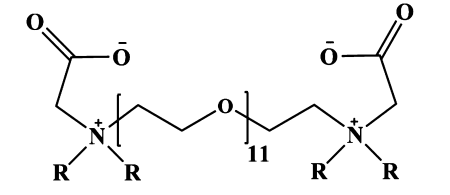
\includegraphics[width=0.7\textwidth]{Graphics/ZLZamudio.png}

\caption[Molécula zwitterion propuesta]{Estructura general de la molécula zwitteriónica propuesta por (\cite{AlczarVara2015}).}

\label{fig:ZLZamudio}

\end{figure}


En este trabajo se presenta el estudio experimental sobre el desempeño a través de sus propiedades de una nueva clase de líquido zwitteriónico, como agente surfactante para la recuperación avanzada.
La estructura química más general del \textbf{LZ} utilizado en este trabajo se muestra en la \autoref{fig:ZLZamudio}, esta molécula pertenece a un desarrollo reciente de surfactante geminal zwitteriónico alquilbetaino con espaciadores de polietileno (\cite{AlczarVara2015}).


%\section{Motivación}
%
%\section{Distribución del aceite en yacimientos}

%Como es un yacimiento (fracturados, múltiple porosidad )
%Como se distribuye el aceite y el agua
%Formación de emulsiones naturales (presencia de agua, )
%Surfactantes
%Los efectos descritos anteriormente pueden ser controlados por medio de la inyección de químicos al yacimiento. A continuación se describen los principales producto utilizados de manera comercial para este fin.
% naturales (resinas y los asfaltenos)
%
%Dado que se tienen lo dos fluidos en contacto, que pueden emulsionarse o separarse, pueden ocurrir diversos escenarios, como la producción de crudo emulsionado, el incremento en la cantidad de agua en la producción debido a l fenomeno conocido como canalización (ref) o la formación de precipitados de sales inorgánicas.



\section{Objetivos}
\begin{description}
\item[General] Proponer un mecanismo para la formación de un organogel formado por la interacción de un surfactante zwitteriónico, agua congénita y aceite provenientes de un yacimiento mexicano, utilizado para la recuperación mejorada de crudo, en base a la determinación de propiedades reológicas, estabilidad de las fases formadas, tiempos de drenado y tensión interfacial.

\clearpage

\item[Específicos] \hfill
  \begin{itemize}
    \item \textbf{Evaluar} el drenado del organogel, durante el reposo a temperatura controlada.
    \item \textbf{Determinar} los parámetros de medición, que permitan mejorar la repetividad en las mediciones reológicas.
    \item \textbf{Correlacionar} las propiedades reológicas con la morfología de las fases obtenida mediante microscopía óptica. 
    \item \textbf{Medir} la tensión superficial y tensión interfacial para las fases presentes en el sistema para su posible correlación con el comportamiento reológico.
    %\item \textbf{Determinar} el contenido de agua del organogel y su relación con la concentración de producto químico.
  \end{itemize}
 
%\section{Metas}
 
%\item[Metas] Como metas específicas del trabajo están la publicación de un artículo técnico en una revista científica, así como la defensa del trabajo de tesis para obtener el grado de maestría.
\end{description}
%
%\section{Contenido de la tesis}
%\chapter{Antecedentes}
\label{chp:antecedentes}

\section{Introducción}
En este capítulo se abordan las generalidades sobre el origen del agua producida y los conceptos como la canalización y conificación de agua en yacimientos naturalmente fracturados. Luego se presenta una breve recopilación de la metodología que existe para su control y remediación. Adicionalmente, se introduce al espacio de los sistemas multifásicos dispersados con la idea de poner en contexto su aplicación en procesos de producción en pozos petrolíferos. Finalmente, se revisan algunos conceptos importantes relativos a las propiedades de la matriz poroso y a la interacción con los fluidos del yacimiento.

\section{Origen del agua producida}
Independientemente del tipo de fluido que se produce de un yacimiento, el agua comúnmente referida como \emph{intersticial} ó \emph{congénita} está presente en el yacimiento dentro de los poros que son suficientemente pequeños para retenerla mediante fuerzas capilares.

Dado que las rocas de un yacimiento son en su mayoría de origen sedimentario, se sabe que el agua se encontraba presente junto con el sedimento previo a los procesos diagenéticos, y por ello fue atrapada en los poros de la roca. Esta agua también puede moverse o pudo haber migrado debido a las presión hidráulica inducida por los procesos geológicos que también forman los yacimientos (\cite{Water1}). En los yacimientos de hidrocarburos siempre existirá una parte de esta agua que no fue desplazada hacia un horizonte acuífero por la migración del petróleo (\cite{StandardHandbook}).

Se sabe que la cantidad de agua intersticial suele ser inversamente proporcional a la permeabilidad del depósito. El contenido de agua congénita en los depósitos productores de hidrocarburos varia a menudo del $10\%$ al $40\%$.

Casi todos los yacimientos productores de hidrocarburos están rodeados por formaciones saturadas de agua llamadas acuíferos Estos acuíferos pueden ser sustancialmente más grandes que los depósitos de aceite y/o gas adyacentes de manera que parecieran de tamaño infinito, o pueden ser tan pequeños que sus efectos sean insignificantes sobre el comportamiento del yacimiento (\cite{Tarek}).

A medida que los fluidos del yacimiento son producidos y la presión del yacimiento declina, se crea un diferencial de presión del acuífero asociado hacia el yacimiento. Siguiendo las leyes básicas del flujo de fluidos en medios porosos, el acuífero reacciona invadiendo el yacimiento a través del contacto agua aceite. Este proceso resulta conveniente para la producción de aceite y gas, dado que cada barril de fluido producido será reemplazado por un barril de agua lo que mitiga la despresurización prematura del yacimiento e incrementa el factor de recuperación.

Esta invasión depende tanto de la permeabilidad del acuífero, que gobierna el diferencial de presión necesario para que la entrada de agua ocurra, así como del tamaño del acuífero en relación con el del yacimiento.

El agua producida en un pozo también puede provenir de pozos inyectores vecinos, ya que la inyección de agua es una de las operaciones mas comunes de la  recuperación secundaria, esta agua inyectada tiene la función de reemplazar dentro de la roca los fluidos que son producidos, de manera que hace mas eficiente el barrido del aceite y gas hacia los pozos.

\section{Problemática}
Se estima que a nivel mundial por cada barril de de petróleo producido se produce con el tres barriles de agua (\cite{Seright2001}). El costo anual por el manejo de agua producido le cuesta a la industria petrolera alrededor de $50$ mil millones de dolares (\cite{Hill2012}), este costo incluye tanto la descarga, el transporte reinyección y tratamiento para la correcta disposición del agua de producción. Este costo sin embargo no captura el costo indirecto asociado con la perdida o retraso de la producción debido a :

\begin{itemize}
    \item Pérdida de producción por aumento de la columna hidrostática.
    \item Flujo preferencial de agua sobre el aceite.
    \item Falta de capacidad en instalaciones para el manejo de agua.
    \item Migración de finos.
    \item Incidentes mecánicos asociados con corrosión y depósitos inorgánicos.
    \item Cierre y abandono de intervalos y pozos.
\end{itemize}

Los problemas asociados con la producción excesiva de agua se han clasificado en al menos $10$ categorías generales (\cite{Bailey2000}).



\subsection{Fugas}
Incluidas las fugas por detrás de la tubería de revestimiento empacadores y tubería de producción, permiten la entrada de agua de zonas no productoras de hidrocarburos hacia la corriente de producción (\autoref{fig:agua1}). En este caso la detección del problema y la aplicación de una solución dependen en gran medida de la configuración y estado mecánico del pozo. Los registros de producción como los de temperatura, densidad y los giroscópicos normalmente son suficientes para el diagnostico de este problema.

\begin{figure}\centering
    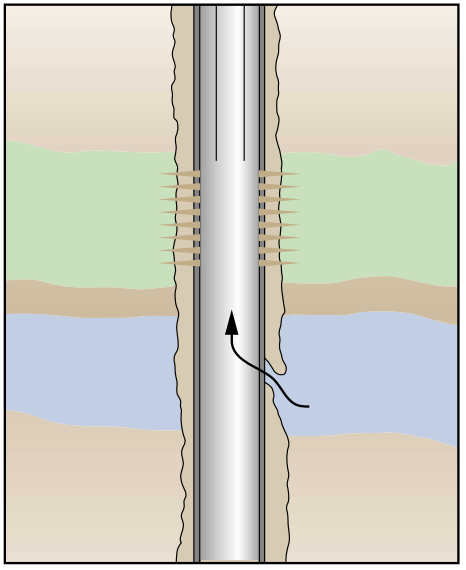
\includegraphics[width=0.5\textwidth]{Graphics/agua1.png}
    \caption[Fugas dentro del pozo]{Ejemplo de una fuga a través del revestimiento, \emph{tubing} o empacador. \emph{Adaptado de (\cite{Bailey2000})}.}
    \label{fig:agua1}
\end{figure}

\subsection{Canalización detrás del revestimiento}
Una cementación fallida puede conectar zonas acuíferas con intervalos productores (\autoref{fig:agua2}). Estos canales de flujo permiten que el agua fluya detrás de la tubería de revestimiento por el espacio anular. Otra posible causa de la canalización, puede ocurrir cuando la producción de arena  genera el derrumbamiento del pozo y crea un área vacía detrás del revestimiento propiciando el flujo de agua).

\begin{figure}\centering
    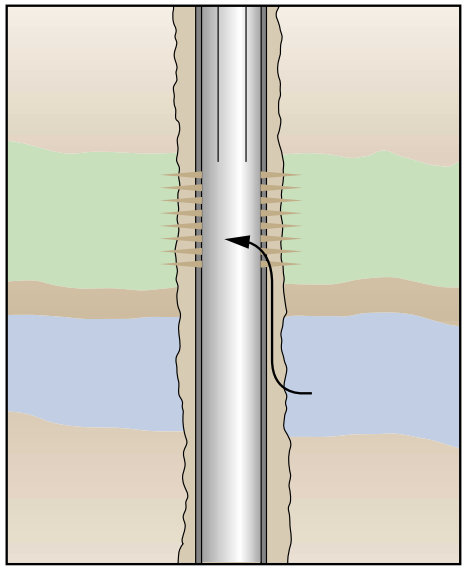
\includegraphics[width=0.5\textwidth]{Graphics/agua2.png}
    \caption[Canalización detras del revestimiento]{Ejemplo de canalización detrás del revestimiento. \emph{Adaptado de (\cite{Bailey2000})}.}
    \label{fig:agua2}
\end{figure}

\subsection{Contacto agua-aceite móvil}
Durante la producción en un yacimiento con empuje de acuífero asociado, el contacto agua aceite avanzando hacia la zona perforada puede resultar en una producción de agua económicamente insostenible. Este fenómeno puede ocurre en formaciones con permeabilidades verticales tan bajas como $K_{v}<0.01[mD]$, dado que el movimiento del contacto ocurre de manera lenta (\autoref{fig:agua3}).

\begin{figure}\centering
    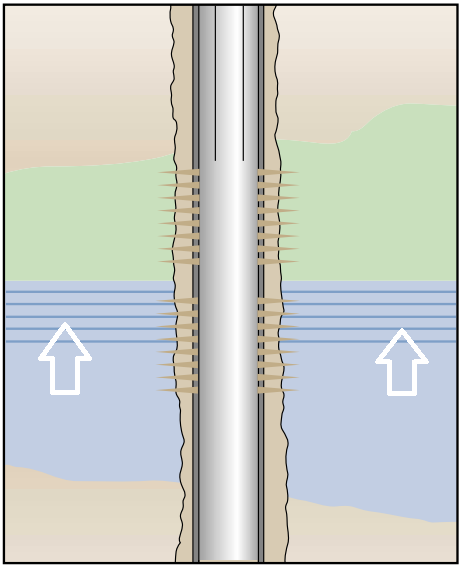
\includegraphics[width=0.45\textwidth]{Graphics/agua3.png}
    \caption[Movimiento del contacto agua aceite]{Movimiento del contacto agua aceite. \emph{Adaptado de (\cite{Bailey2000})}.}
    \label{fig:agua3}
\end{figure}


\subsection{Capa de riego sin flujo transversal}
Un problema común durante la producción simultanea de intervalos ocurre cuando un estrato o zona de alta permeabilidad que posee una barrera de flujo (como una capa de lutita) conduce el agua directamente hacia el pozo productor (\autoref{fig:agua4}). La fuente del agua puede ser un acuífero activo o un pozo inyector. Como no existe el flujo transversal este problema puede ser fácilmente atacado mediante agentes gelantes o selladores mecánicos dentro del pozo.

\begin{figure}\centering
    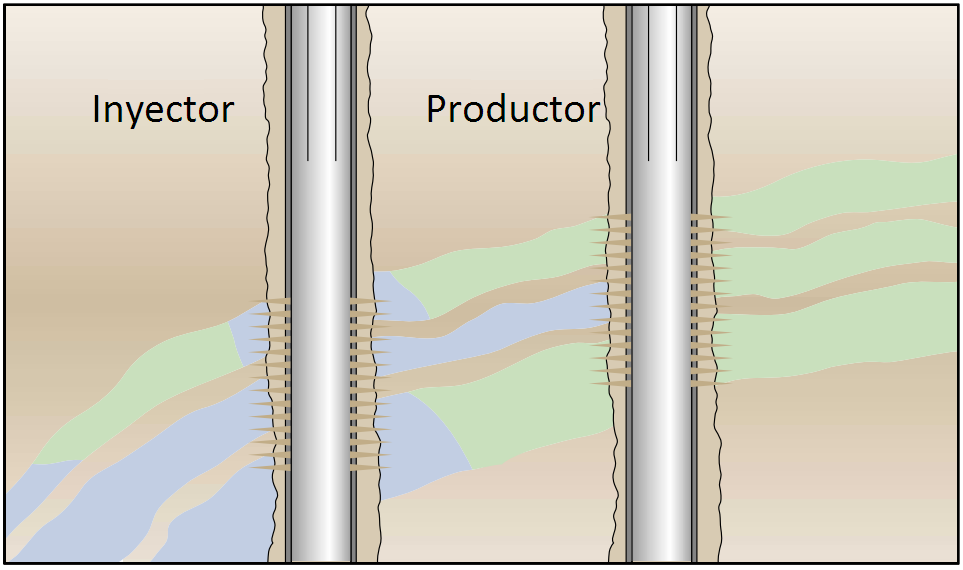
\includegraphics[width=0.8\textwidth]{Graphics/agua4.png}
    \caption[Capa de riego sin flujo transversal]{Capa de riego sin flujo transversal entre intervalos. \emph{Adaptado de (\cite{Bailey2000})}.}
    \label{fig:agua4}
\end{figure}


%\subsection{Digitalización}
\subsection{Fallas y fracturas entre inyector y productor}
En formaciones naturalmente fracturadas, la inyección de agua puede rápidamente avanzar hasta los pozos productores ()\autoref{fig:agua5}. Esto es común cuando el sistema de fracturas es extenso o fisurado y puede ser confirmado mediante el análisis de pruebas de presión y el uso de trazadores. Los registros de trazadores pueden también estimar el volumen de fracturas para diseñar el método de remediación. El uso de geles ha demostrado ser una opción viable para mitigar la producción excesiva de agua.

\begin{figure}\centering
    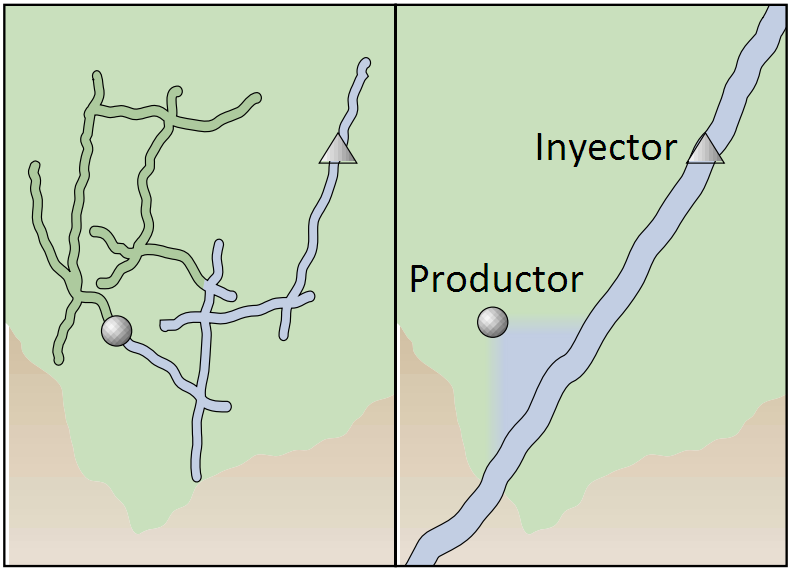
\includegraphics[width=0.65\textwidth]{Graphics/agua5.png}
    \caption[Fracturas de inyector a productor]{Aporte de agua por fallas y fracturas entre pozos inyector y productor. \emph{Adaptado de (\cite{Bailey2000})}.}
    \label{fig:agua5}
\end{figure}

\subsection{Fallas y fracturas desde un acuífero}
El agua puede ser producida desde fracturas que interconectan zonas acuíferas mas profundas con el intervalo disparado (\autoref{fig:agua6}). Estas fracturas pueden ser obturadas cuando no aportan aceite a la producción, sin embargo el reto radica en que no se conoce el tamaño del volumen fracturado. Este caso es mas común en pozos terminados horizontalmente.

\begin{figure}\centering
  \subfloat[pozo vertical]{
    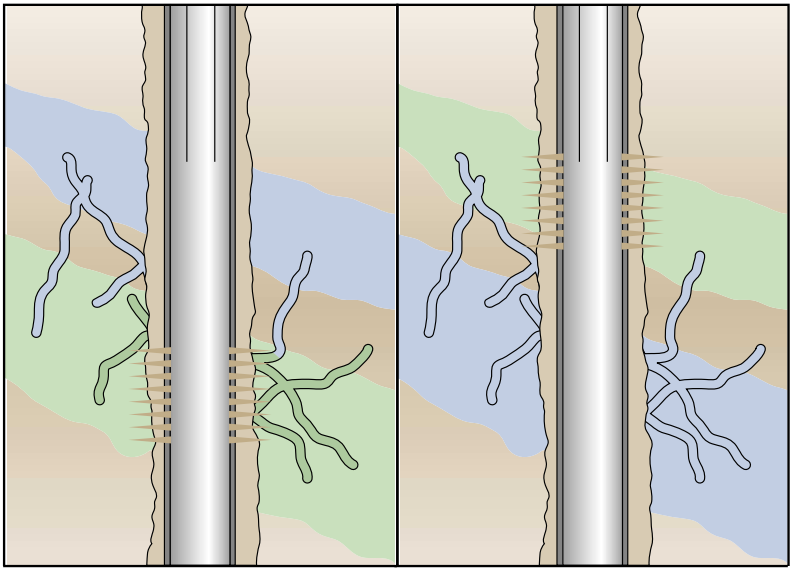
\includegraphics[width=0.45\textwidth]{Graphics/agua6a.png}} \quad
  \subfloat[pozo horizontal]{
    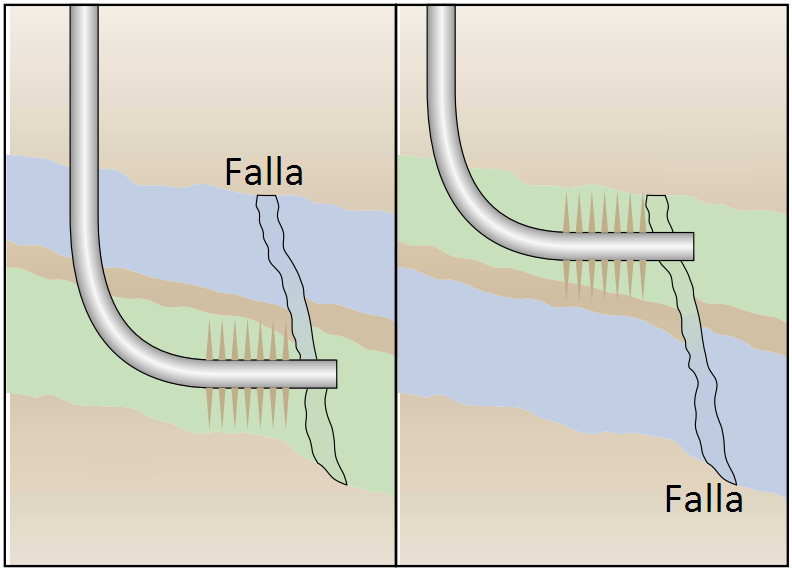
\includegraphics[width=0.45\textwidth]{Graphics/agua6b.png}} 
  \caption[Fallas y fracturas desde un acuifero]{Aporte de agua por fallas y fracturas desde un acuífero mas profundo \textbf{a)} y desde un acuífero mas somero \textbf{b)} . \emph{Adaptado de (\cite{Bailey2000})}.}
  \label{fig:agua6}
\end{figure}

\subsection{Conificación y Dunas}
La conificación es principalmente el resultado del movimiento de los fluidos del yacimiento en la dirección de menor resistencia, equilibrada por una tendencia de los fluidos a mantener la segregación gravitacional. 

En un pozo vertical ocurre a menudo cuando la zona disparada se encuentra cerca del contacto agua aceite en una formación con permeabilidad vertical relativamente alta. Existe un ritmo de producción máximo para no producir agua a través de un cono, pero este siempre es muy bajo para ser económicamente factible. En pozos horizontales este problema es referido como duna o cresta (\autoref{fig:agua7}).

\begin{figure}\centering
    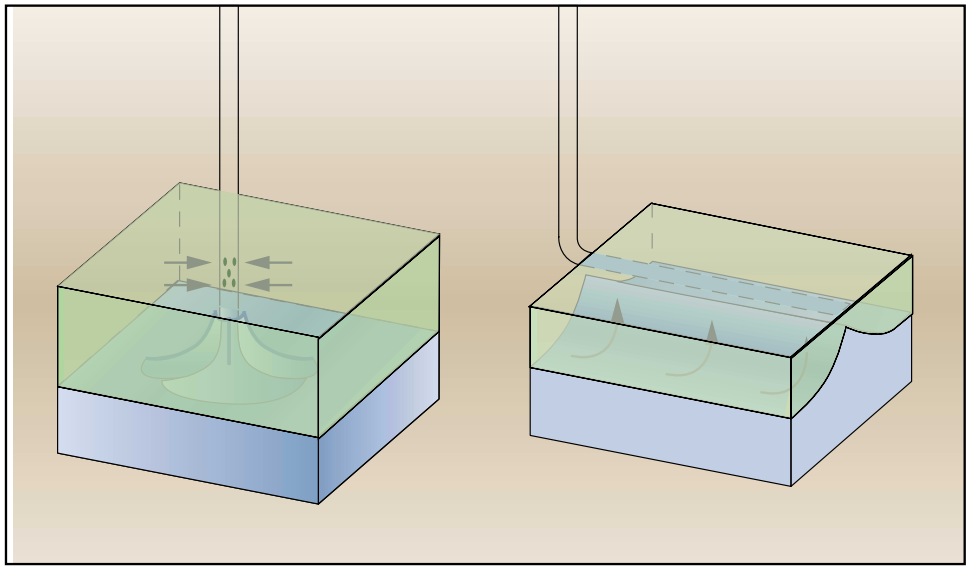
\includegraphics[width=0.65\textwidth]{Graphics/agua7.png}
    \caption[Conificación y dunas]{Conificación de agua en pozos verticales y \emph{dunas} en pozos horizontales. \emph{Adaptado de (\cite{Bailey2000})}.}
    \label{fig:agua7}
\end{figure}

\subsection{Barrido areal deficiente}
Un acuífero o pozo inyector de agua muy cercano a la zona impregnada de aceite a menudo provoca un barrido areal deficiente (\autoref{fig:agua8}). La heterogeneidad de la formación y anisotropía es la principal causa de este problema que es muy frecuente en depósitos de canal en arenas.

\begin{figure}\centering
    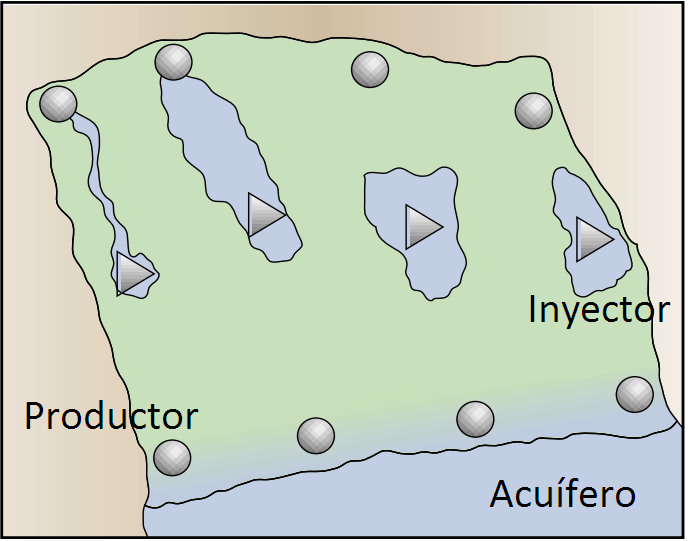
\includegraphics[width=0.63\textwidth]{Graphics/agua8.png}
    \caption[Barrido areal deficiente]{Los pozos productores cercanos al acuífero rápidamente serán invadidos por agua, mientras que las heterogeneidades del yacimiento y la diferencia de permeabilidades entre estratos y facies provoca que el agua no desplace de manera eficiente al aceite hacia los pozos. \emph{Adaptado de (\cite{Bailey2000})}.}
    \label{fig:agua8}
\end{figure}

\subsection{Capa con segregación gravitacional}
En un yacimiento de gran espesor con buena permeabilidad vertical, la segregación gravitacional de fases (agua-aceite) puede provocar un aporte de agua desfavorable hacia el pozo productor. El agua proveniente de un acuífero activo o pozo inyector, se infiltra en la parte baja de la formación permeable barriendo únicamente una parte del aceite del yacimiento al pozo (\autoref{fig:agua9}). Una baja movilidad del aceite y formaciones con texturas sedimentarias mas finas en la parte superior pueden empeorar el problema, pues los efectos viscosos y la segregación favorecen el flujo de agua en la parte baja del yacimiento.

\begin{figure}\centering
    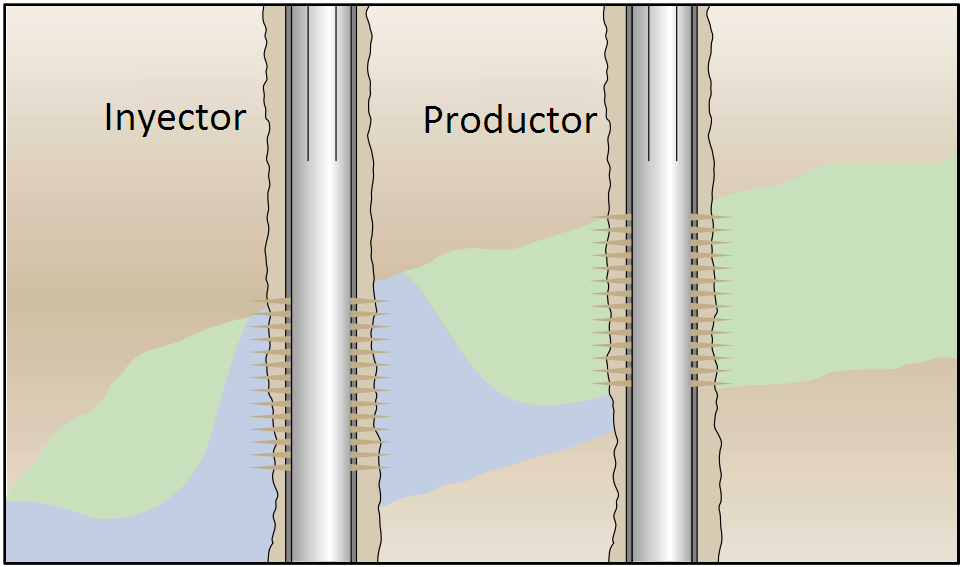
\includegraphics[width=0.65\textwidth]{Graphics/agua9.png}
    \caption[Capa con segregación gravitatacional]{Capa de riego con aporte de agua por debajo del aceite debido a la segregación gravitacional. \emph{Adaptado de (\cite{Bailey2000})}.}
    \label{fig:agua9}
\end{figure}

\subsection{Capa de riego con flujo transversal}
El flujo transversal puede ocurrir en formaciones que presentan capas con alta permeabilidad que no se encuentran aisladas una de otra por barreras impermeables \autoref{fig:agua10}.

\begin{figure}\centering
    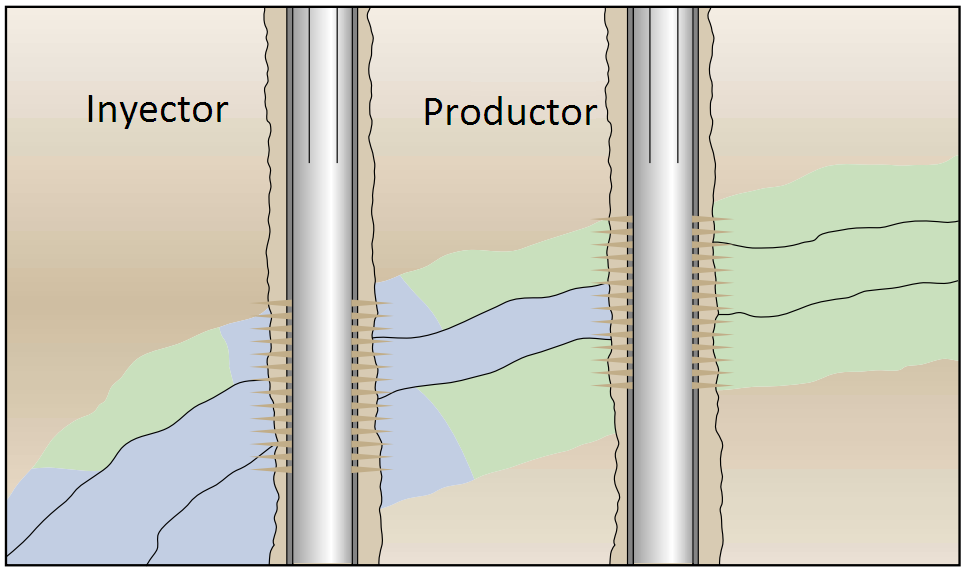
\includegraphics[width=0.65\textwidth]{Graphics/agua10.png}
    \caption[Capa de riego con flujo transversal]{En el caso del flujo transversal al no haber barreras impermeables entre estratos o capas, aislar la capa de riego no resolverá el problema. \emph{Adaptado de (\cite{Bailey2000})}.}
    \label{fig:agua10}
\end{figure}


\section{Técnicas de control y mitigación de la producción de agua}
Existen básicamente tres enfoques distintos para el control de agua producida en exceso, soluciones mecánicas, químicas y operaciones mas complejas y costosas que incluyen cambios en el estado mecánico del pozo o el aparejo de producción. En ocasiones mas de un problema esta presente, por lo que una combinación de técnicas deben ser implementadas.

De manera general \cite{Seright2001} agrupa en tres categorías donde se distingue la problemática a atacar y la solucion recomendada de uno o mas problemas como se muestra en la \autoref{tab:agua1}.

\begin{table} \caption[Categorias: Problemática y tratamiento]{Categorías de problemas de producción de agua excesiva y su tratamiento. Adaptada de (\cite{Seright2001}). }
        \begin{tabulary}{\textwidth}{LL}
            \multicolumn{2}{l}{Categoría \textbf{A} Tratamientos mecánico}\\ 
            \midrule              
             $\bullet$ & Fugas en el revestimiento \\
             $\bullet$ & Canalización detrás del revestimiento\\
        \end{tabulary} 
    \\ \vspace{0.5cm}
        \begin{tabulary}{\textwidth}{LL}
            \multicolumn{2}{l}{Categoría \textbf{B} Tratamiento con geles}\\ 
            \midrule              
            $\bullet$ & Conificación del acuífero a través de una fractura\\
            $\bullet$ & YNF con acuífero asociado \\
            $\bullet$ & Fuga a través del revestimiento \\
        \end{tabulary}
    \\ \vspace{0.5cm}
    \begin{tabulary}{\textwidth}{LL}
        \multicolumn{2}{l}{Categoría \textbf{C} Tratamiento con geles preformados}\\ 
        \midrule              
        $\bullet$ & Fallas o fracturas que cruzan pozos horizontales \\
        $\bullet$ & Una fractura causante de canalización entre dos pozos\\
        $\bullet$ & YNF causando canalización entre dos pozos \\
    \end{tabulary}
    \\ \vspace{0.5cm}
\begin{tabulary}{\textwidth}{LL}
    \multicolumn{2}{l}{Categoría \textbf{D} Casos especiales}\\ 
    \midrule              
    $\bullet$ & Conificación de agua \\
    $\bullet$ & Dunas de agua (pozo horizontal) \\
    $\bullet$ & Aporte de agua por capas de riego\\
\end{tabulary}
    \label{tab:agua1}
\end{table}

\subsection{Soluciones mecánicas}
En muchos de los casos donde el problema se encuentra cercano al agujero de pozo, como fugas detrás del revestimiento o capas de riego sin flujo transversal, se aisla el intervalo por medio de tapones mecánicos o inflables, así como también cementaciones que pueden ser colocadas en agujeros descubiertos o entubados. Los detalles de estas operaciones pueden ser consultados en otros trabajos (\cite{SLB:2014}).

\subsection{Métodos químicos}
Esta categoría consta básicamente de incluye los químicos formadores de geles y en ocasiones su mezcla con cemento (\cite{SLB:2011}).

\begin{description}
    \item[Geles acuosos] Son formados por polímeros sintéticos y geles reticulantes, se utilizan en yacimientos naturalmente fracturados, donde se produce un alto corte de agua a través de las fracturas. Son de peso molecular alto lo cual limita las pérdidas de gel en la matriz y da como resultado viscosidades altas penetrando en las fracturas naturales.
    \item[Geles rígidos] Consisten en un sistema que produce un gel polimérico sintético reticulado de gran fuerza el cual es capaz de penetrar en la matriz antes de gelificarse. Se utiliza cuando se requiere la obstrucción completa de la vecindad del pozo por canalizaciones, canales de alta permeabilidad y abandono de zonas.
    \item[Lechadas selectivas] Estas lechadas están compuestas por cemento microfino suspendido en un medio orgánico (solventes y surfactantes). Esta composición provee la característica de mantenerse en fase líquida, es decir sin adquirir consistencia de fraguado ni de desarrollar gelificación, mientras no entre en contacto con agua. En los canales mojados con aceite esta lechada se mantendrá en estado líquido, lo cual permitirá removerla fácilmente; en cambio al contacto con agua el cemento se empezará gelificar y posteriormente a fraguar.
    \item[Modificadores de la permeabilidad relativa] consiste en un polímero (normalmente catiónico) soluble en salmuera acuosa. La absorción del polímero reduce la sensibilidad  en las arcillas y areniscas al intercambio catiónico, reduciendo la permeabilidad relativa al agua y minimizando el cambio de permeabilidad relativa al aceite.
\end{description}


\section{Sistemas Dispersados}
El concepto de sistema dispersado fue introducido por primera por \cite{Ostwald} y \cite{Weimarn} en su intento por estudiar las propiedades de los coloides. Un sistema dispersado incluye cualquier medio homogéneo, que contiene entidades dispersas de cualquier tamaño y en cualquier estado (\cite{ShortText}). Los coloides y su vez las emulsiones pueden ser contenidos dentro de esta definición. Las propiedades y el comportamiento de estos sistemas esta relacionado con el tamaño y la forma de las partículas dispersas. La primera clasificación para los sistemas dispersados se basaba en el tamaño de las partículas \autoref{tab:coloid1}. Estos límites fueron arbitrariamente escogidos por Ostwald, aunque las propiedades coloidales pueden presentarse en partículas mucho mas grandes de hasta $0.0005 mm$.

 \begin{table} 
 \caption[Sistemas dispersados]{Clasificación de los sistemas dispersados. Adaptada de (\cite{ShortText}).}
     \centering
     \begin{tabulary}{\textwidth \tymin=99.73pt}{L C L}
     \toprule
        \multicolumn{3}{c}{Sistemas Dispersados}\\\midrule%
        Dispersiones gruesas & Dispersiones coloidales & Moléculas pequeñas y átomos\\%
        ~ $>0.1 \mu$ m  & $0.1 \mu$ m - $10 A$  & $< 10 A$ \\%
         ~ \tikzmark{a} & ~ & \tikzmark{b}\\%
     \bottomrule
     \end{tabulary}     
     \label{tab:coloid1}
  \end{table}
  
  \begin{tikzpicture}[overlay, remember picture] 
     \draw[thick,->] (a) -- (b) node[label=right:{\textit{menor tamaño}}]{};
  \end{tikzpicture}

Dado que algunas moléculas, como por ejemplo la celulosa, poseen dimensiones de $0.0015$ mm de longitud, pero $8x10^{-7}$ mm ($8$ A) de espesor, pueden ser clasificadas por su longitud dentro de las dispersiones gruesas, mientras que su espesor está cerca de ser una dispersión molecular. Para sobreponerse a esta problemática una nueva clasificación para los sistemas dispersados (\cite{Staudinger}), fue propuesta para tomar en cuenta el número de átomos que componen a la fase dispersada y no el tamaño de las partículas \autoref{tab:coloid2}.
 
 
  \begin{table}
 \caption[Sistemas dispersados]{\raggedright Propiedades de los sistemas dispersados. Adaptada de (\cite{ShortText}).}
     \centering \footnotesize
     \begin{tabulary}{\textwidth \tymin=99.73pt}{L|L|L}
     \toprule 
        Dispersiones gruesas & Coloides &  Moléculas pequeñas y átomos\\ 
        \midrule              
        Partículas compuestas de más de $10^9$ átomos. &  Partículas compuestas de $10^3$-$10^9$ átomos. & Moléculas que contienen $1$-$10^3$ átomos.\\
        
        Partículas visibles en un microscopio ordinario. &  Partículas son visibles en microscopio electrónico y ultramicroscopio, no detectables en microscopio ordinario. & Invisibles en microscopio electrónico.\\ 
        
        Partículas retenidas en papel filtro ordinario. &  Partículas atraviesan papel filtro pero son retenidas en ultra filtros. &  Atraviesan ultra filtros.\\
        
        Partículas no se dializan ni se difunden. &  Muy poca difusión, solo las partículas mas pequeñas se dializan muy lentamente. &  Rápida difusión y diálisis a través de membranas.\\
     \midrule
     \bottomrule
     \end{tabulary}
     \label{tab:coloid2}
\end{table}
 

\subsection{Coloides}

Si bien los coloides son una clasificación de los materiales muy amplia y no existe una estricta definición, en la literatura actual podemos encontrar definiciones de coloide como:

\begin{description}

\item[(\cite{ShortText})] \protect \raggedright Un coloide en su estructura mas básica consiste de un medio homogéneo con partículas dispersadas dentro de el.
\item[(\cite{ColloidSurface})] Cualquier partícula que posea una dimensión lineal entre $10^{-9}m$ ($10$A) y $10^{-6}m$ ($\mu m$).
\item[(\cite{Drew})] Los coloides son, en general, sistemas que consisten en una sustancia (sólido líquido o gas) finamente dividido y distribuido uniformemente, dentro de una segunda sustancia (sólido líquido o gas).
\item[(\cite{Handbook})] Los coloides son pequeñas partículas rodeadas de fluido con al menos una de sus dimensiones dentro del rango submicrónico y que poseen carga eléctrica superficial.

\end{description}


\begin{figure}
\centering
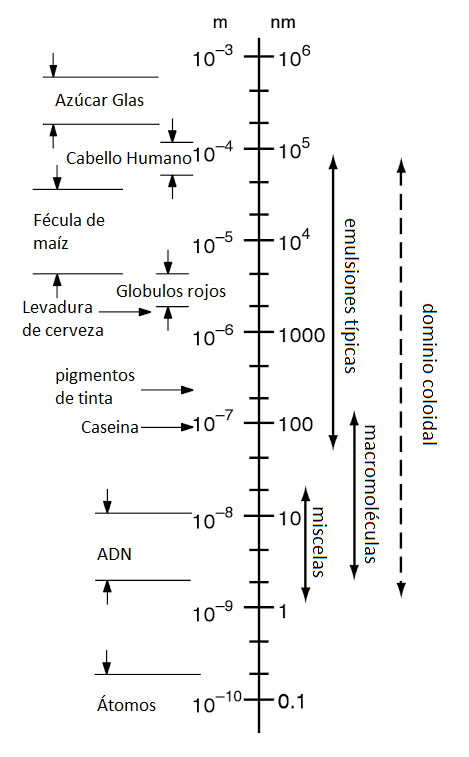
\includegraphics[width=\textwidth]{Graphics/Espectro.png}
\caption[Dominio coloidal]{Dominio coloidal: sus dimensiones y ejemplos típicos de materiales que caen dentro del rango coloidal. Adaptado de (\cite{Cosgrove}). }
\label{fig:Domain}
\end{figure}

De manera que podemos pensar en un coloide como un sistema compuesto por dos sustancias mezcladas de manera especial, donde una de ellas se encuentra dispersa en la otra, donde además la dispersión debe cumplir con ciertos requerimientos de tamaño, en la \autoref{fig:Domain} se muestra el espectro de dimensiones coloidal. Sin embargo en la práctica muchos sistemas con dimensiones que van mas allá del rango de tamaño establecido anteriormente, particularmente las emulsiones, también son incluidos dentro de los coloides, dado que sus características así lo permiten. En este sentido algunos sistemas como las fibras, arcillas y películas delgadas pueden calificar como coloides puesto que alguna de sus dimensiones cae dentro del rango especificado de tamaño y además sus propiedades se asemejan a las del comportamiento coloidal, la (\autoref{fig:Dimensions}) esquematiza este concepto.

% In practice, however, many systems with dimensions beyond that range, in
% particular most emulsions, paints, and aerosols, must also be included under
% the colloid umbrella, since their characteristics allow no other realistic option.
% Other colloidal systems, such as fibers, clays, and thin films, may ‘‘qualify’’ as
% colloids because one or two dimensions fall into the designated range, and
% their properties adhere to the ‘‘rules’’ of colloidal behavior. That concept is
% illustrated schematically in Figure 10.1. Ultimately, the most useful definition
% to use is that if it looks like a colloid and acts like a colloid, it is a colloid,
% regardless of other more restrictive limitations

\begin{figure}
\centering
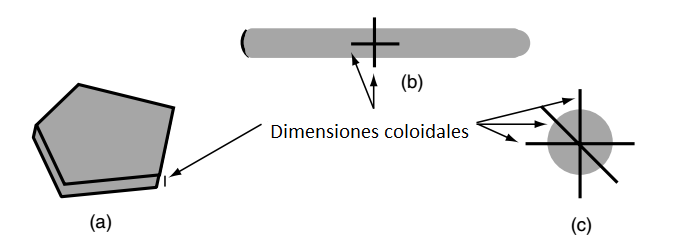
\includegraphics[width=\textwidth]{Graphics/Dimensiones.png}
\caption[Dimensiones coloidales]{Un coloide esta definido básicamente por sus dimensiones. Muchos sistemas con proporciones mucho mas grandes son aun considerados como típicos coloides puesto que al menos una de sus dimensiones cae dentro del rango límite de tamaño como en una placa delgada \textbf{(a)} un cilindro \textbf{(b)} o una gota \textbf{(c)}. Adaptado de (\cite{Drew}). }
\label{fig:Dimensions}
\end{figure}

Los sistemas coloidales pueden ser agrupados en tres clasificaciones generales (\cite{Duncan}):
\begin{description}
  \item[Dispersiones coloidales]
    Son termodinamicamente inestables debido a su alta energía libre superficial, y son sistemas irreversibles en el sentido de que no pueden ser fácilmente reconstituidos después de una separación de fases.
  \item[Soluciones macro moleculares] 
    Son termodinamicante estables y son sistemas reversibles en el sentido de poder reconstituirse con facilidad luego de haber ocurrido la separación del soluto y el solvente.
  \item[Coloides Asociados] 
    % Están relacionados con la formación de estructuras miscelares. Surface-active molecules or surfactants, such as soaps, detergents and lipids, can self-assemble to form multi-molecular aggregates of colloidal size and show the effects of colloidal forces in addition to their individual phase behaviour 
    Las moléculas tensoactivas o surfactantes, como jabones, detergentes y lípidos, pueden auto estructurarse (ensamblarse) para formar agregados multimoleculares de tamaño coloidal y mostrar los efectos de las fuerzas coloidales adicionalmente de su comportamiento de fase individual
    (\cite{Goodwin}).
\end{description}

Algunos ejemplos de coloides encontrados cotidianamente son: leche (grasa liquida dispersada en finas gotas dentro de una fase acuosa), humo (partículas sólidas dispersas en aire), niebla (pequeñas gotas de líquido dispersas en aire), pinturas (pequeñas partículas sólidas dispersas en líquido), geles (moléculas de polímero que, cuando son disueltas en un solvente, proporcionan una estructura semi-sólida a la solución), y hueso (pequeñas partículas de fosfato de calcio dispersas en una matriz sólida de colágeno). Una terminología alrededor del estado de agregación de las sustancias presentes en dispersiones coloidales se muestra en la tabla \autoref{tab:coloid3}.

%\subsection{Clasificación de las dispersiones coloidales}

Dispersiones coloidales con desviación estándar del tamaño medio de partícula menor al $10\%$, se consideran como \emph{monodispersas}. Si la distribución del tamaño medio de partícula es mas amplia, entonces la dispersión es \emph{polidispersa}. Aunque esta clasificación es un tanto arbitraria, los sistemas monodispersos tienen la habilidad de formar cristales coloidales mientras que los polidispersos no pueden. Los sistemas que presentan una distribución del tamaño de partícula bimodal también pueden formar estructuras cristalinas.

% Colloidal dispersions in which the standard deviation on the mean size is less than 10\% of the mean are usually considered to be ‘monodisperse’. If the particle size distribution is broader than this, the dispersion is considered to be ‘polydisperse’. Although this cut-off appears arbitrary, monodisperse systems have the ability to form colloidal crystals whereas polydisperse systems do not. Bimodal systems can also form crystalline structures if the size ratio is suitable. 

\cite{Freundlich} sugiere que las dispersiones coloidales pueden ser divididas en dos clases llamadas \emph{liofílicas} (afinidad al solvente) y \emph{liofóbicas} (repulsivas al solvente) respectivamente, dependiendo de la facilidad con que dicho sistema puede ser redispersado una vez que esta seco.   
% Freundlich, in his classical text on the subject (1926), suggested that colloidal
% dispersions could be divided into two classes, called lyophilic (solvent loving) and
% lyophobic (solvent hating) respectively, depending on the ease with which the system
% could be redispersed if it was allowed to dry out.
\cite{Kruyt} usa la misma clasificación y se refiere a ellos como sistemas reversibles e irreversibles, respectivamente. Esta terminología es particularmente útil cuando se considera el fenómeno de actividad superficial. Las moléculas de materiales tensoactivos tienen una fuerte afinidad por las interfaces, dado que contienen ambas regiones liofílicas y liofóbicas.
% Esta This terminology is particularly useful when one considers the phenomenon of surface activity. The molecules of surface-active materials have a strong affinity for interfaces, because they contain both hydrophilic and lipophiiic (oil-loving) regions.
% De esta manera queda mas clara la naturaleza de esta distinción dado que la prueba máxima para saber que un sistema es liofílico consiste en determinar si el proceso de dispersión ocurre de manera espontánea cuando el disolvente es añadido al coloide.  
% Kruyt (1952) uses the same classification and
% refers to them also as reversible and irreversible systems, respectively. This
% terminology expresses more clearly the real nature of the distinction because the
% ultimate test of whether a system is lyophilic is to determine whether the dispersion
% process occurs spontaneously when the solvent is added to the colloid.
Otro factor que distingue el comportamiento de los sistemas reversibles (liofílicos) e irreversibles (liofóbicos) es la medida en la cual el medio de dispersión (disolvente) es capaz de interactuar con los átomos de la partícula suspendida. Si el solvente puede entrar en contacto con todas o la mayor parte de de esos átomos entonces la energía de solvatación será importante y el coloide debería ser liofílico (reversible) en algún disolvente adecuado. En el caso donde la estructura de las partículas suspendidas (fase dispersa), permite al disolvente entrar en contacto con solo una pequeña fracción de sus átomos, entonces el coloide casi con seguridad será liofóbico (irreversible) en su comportamiento, aun cuando los átomos en su superficie interactúen fuertemente con el disolvente. 

% One contributing factor to the difference in behaviour between reversible(lyophilic) and irreversible (lyophobic) systems is the extent to which the dispersion medium (solvent) is able to interact with the atoms of the suspended particle. If the solvent can come into contact with all or most of those atoms then solvation energy will be important and the colloid should be lyophilic (reversible) in some suitable solvent.

% If the solvent is prevented, by the structure of the suspended particles (i.e. the disperse phase), from coming into contact with any but a small fraction of the atoms of those particles then the colloid will almost certainly be lyophobic (i.e. irreversible) in its behaviour, even if the surface atoms interact strongly with the solvent


  \begin{table}
 \caption[Dispersiones coloidales]{\raggedright Clasificación de las dispersiones coloidales y ejemplos de ellas (\cite{Pashley}).}
     \centering \footnotesize
     \begin{tabulary}{\textwidth}{L|L|L|C}
     \toprule 
        Fase dispersa & Medio &  Nombre & Ejemplos\\ 
        \midrule              
        Líquido & Gas & Aerosol líquido & Nieblas, \emph{sprays}\\
        Sólido & Gas & Aerosol sólido & Humo, polvo\\
        \multicolumn{4}{c}{~}\\
        Gas & Líquido & Espuma & Espumas\\
        Líquido & Líquido & \textbf{Emulsión} & Leche, mayonesa\\
        Solido & Líquido & Suspensión & Tinta\\
        \multicolumn{4}{c}{~}\\
        Gas & Sólido & Espuma sólida & Poliestireno\\
        Líquido & Sólido & Emulsión sólida & Ópalo, perla\\
        Sólido & Sólido & Suspensión sólida & Rubí, mantequilla\\
     \midrule
     \bottomrule
     \end{tabulary}
     \label{tab:coloid3}
\end{table}


% Classification of colloidal systems
% Colloidal systems may be grouped into three general classifications:
% 1. Colloidal dispersions are thermodynamically unstable owing to
% their high surface free energy and are irreversible systems in the
% sense that they are not easily reconstituted after phase separation.
% 2. True solutions of macromolecular material (natural or synthetic)
% are thermodynamically stable and reversible in the sense that they
% are easily reconstituted after separation of solute from solvent.
% 3. Association colloids which are thermodynamically stable (see
% Chapter 4)
%\subsection{Emulsiones}
%
%Las emulsiones son un tipo de dispersión coloidal que de dos líquidos inmiscibles. En una emulsión las gotas de tamaño coloidal formadas de uno de los líquidos (fase dispersa) se encuentran dispersadas dentro de un medio de otro líquido (fase continua). Diferentes clases de emulsiones pueden ser identificadas, entre ellas aceite en agua (\textbf{O/W}), agua en aceite (\textbf{W/O}) y aceite en aceite (\textbf{O/O}) (\cite{Tharwat}).

%\section{Geles}



\section{Conceptos de relevancia en la industria}
Cuando sólo existe un fluido en los espacios porosos de una roca, se considera que solo hay un conjunto de fuerzas activas, que es, la atracción entre la roca y el fluido. En cualquier yacimiento donde esté presente un único fluido, tal como un acuífero, estas fuerzas pueden no ser tan importantes porque la porosidad y la permeabilidad absoluta son en cierta medida suficientes para definir las características de tales depósitos. Sin embargo, cuando hay más de una fase de fluido, es necesario considerar al menos tres conjuntos de fuerzas activas, para un sistema de dos fluidos, las fuerzas a considerar son:
\begin{itemize}
    \item{Fluido1 - Fluido2}
    \item{Fluido1 - Roca}
    \item{Fluido2 - Roca}
\end{itemize}

La existencia de estas fuerzas da lugar a propiedades fundamentales como la tensión interfacial y la mojabilidad. Además la existencia de dos fluidos dentro del espacio poroso introduce otras propiedades como la presión capilar y la permeabilidad relativa. En conjunto estas propiedades son necesarias para describir las características y el potencial de cualquier yacimiento.

Existe una clara dependencia de estas propiedades con la tensión interfacial (mostrada abajo), por lo que se abordan en orden partiendo del concepto mas general.

\begin{figure}[h]
    \centering
    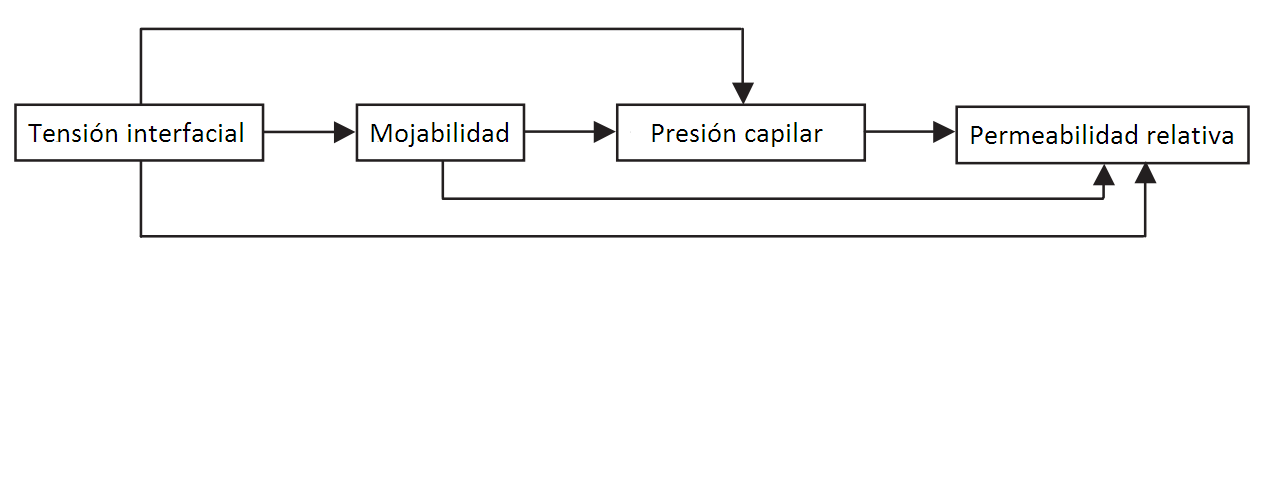
\includegraphics[width=\textwidth]{Graphics/dependencia.png}
%    \caption[Concepto de porosidad]{Dependencia . Adaptado de (\cite{Dandekar}). }
    \label{fig:dependencia}
\end{figure}

\subsection{Porosidad}
Una roca típica de yacimientos como la arenisca es el resultado de granos de arena con diferentes tamaños agrupados como parte del proceso deposicional que forman un consolidado, con espacios vacíos entre granos (\autoref{fig:poro1}). La mayoría de las rocas sedimentarias están conformadas por granos con diámetros que varían en el rango de $0.05$ a $0.25~$ mm, resultando en un promedio de radio de poro (espacios vacíos) de entre $20$ y $200~\mu$m (\cite{Tissot}). Cuanto mayor porosidad posea una roca, esta tendrá mayor cantidad de espacio vacío y por consecuencia mayor capacidad para almacenar los fluidos del yacimiento, es por eso que representa una de las propiedades mas importantes de la roca.

\begin{description}
    \item[Definición] La porosidad ($\phi$) se define como el cociente entre el volumen poroso (espacio vacío) dentro de un roca y su volumen total, expresado en porcentaje.
\end{description}

\begin{equation}
        \phi = \frac{Volumen~ poroso}{Volumen~ total}
\end{equation}

El volumen poroso se refiere a la suma, o el volumen combinado, de todos los espacios de poro presentes en la roca.

\begin{figure}
\centering
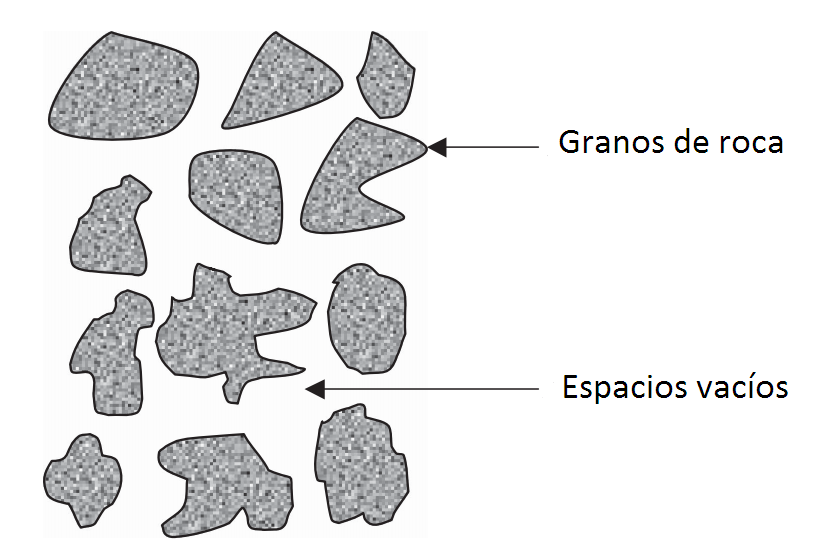
\includegraphics[width=0.7\textwidth]{Graphics/poro1.png}
\caption[Concepto de porosidad]{Representación conceptual del espacio poroso en una roca sedimentaria. Adaptado de (\cite{Dandekar}). }
\label{fig:poro1}
\end{figure}

\subsubsection{Tipos de porosidad}
Algunos de los espacios porosos de una roca pueden estar interconectados con otros poros formando una red, algunos otros pueden estar conectados con poros sin salida, que no conectan con otros poros y también existen espacios porosos que están completamente aislados. Estas características se deben a la variedad de procesos geológicos y deposicionales particulares de cada región y tipo de sedimento, pero en general para las rocas se pueden distinguir tres tipos de poros: interconectados, poros sin salida y poros aislados su representación se muestra en la \autoref{fig:poro2}.

\begin{figure}
    \centering
    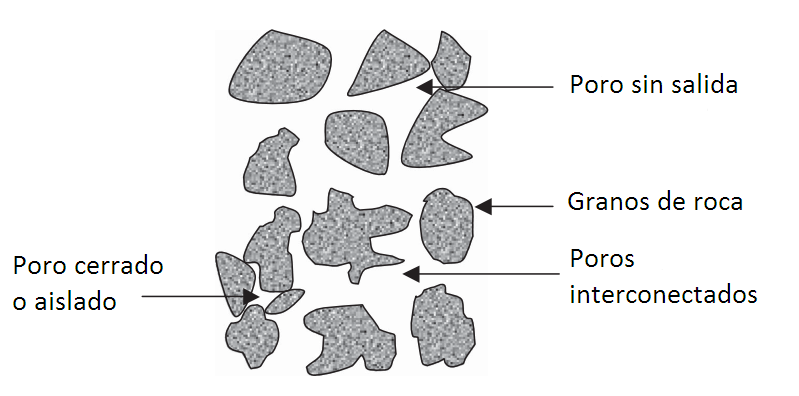
\includegraphics[width=0.9\textwidth]{Graphics/poro2.png}
    \caption[Tipos de porosidad]{Representación conceptual de los tipos de espacio poroso en una roca sedimentaria. Adaptado de (\cite{Dandekar}). }
    \label{fig:poro2}
\end{figure}

En base a estos tres tipos de poros, la porosidad total o absoluta de una roca comprende tanto la porosidad efectiva como la no efectiva en términos de almacenamiento de fluidos.

\subsubsection{Porosidad efectiva}

\begin{description}
    \item[Definición] La porosidad efectiva ($\phi_{EF}$) se define como el cociente de el volumen poroso interconectado y sin salida de una roca entre su volumen total, expresado en porcentaje.
\end{description}

\begin{equation*}
\phi_{EF} = \frac{Vol.~ poros~ interconectados + Vo.~poros~sin salida }{Volumen~ total}
\end{equation*}

Aun cuando la porosidad en algunas rocas carbonatadas es en su mayoría del tipo sin salida, estos poros pueden producir hidrocarburos por medio de la despresurización y expansión del gas.

\subsubsection{Porosidad no efectiva}

\begin{description}
    \item[Definición] La porosidad no efectiva ($\phi_{NOEF}$) se define como el cociente entre el volumen poroso aislado o completamente desconectado de una roca y su volumen total, expresado en porcentaje.
\end{description}

\begin{equation*}
\phi_{NOEF} = \frac{Vol.~ poros~ no conectados }{Volumen~ total}
\end{equation*}

Este tipo de porosidad no es capaz de aportar fluidos durante la producción en un yacimiento.

En general para material con cementación baja o moderada (arenas), la porosidad absoluta será aproximadamente igual a la porosidad efectiva, mientras que para material con muy buena cementación (carbonatos) existirá una diferencia importante debido a que gran parte de la porosidad puede encontrarse completamente aislada del resto.

\subsubsection{Porosidad primaria y secundaria}

Adicionalmente se pueden distinguir dos clasificaciones de porosidad original e inducida, comúnmente referidas como primaria y secundaria. La porosidad original es el resultado de la depositación del material, mientras que la inducida se desarrolla por procesos geológicos que ocurren posterior a la depositación (\cite{Amix}). Ejemplos de porosidad secundaria son las fracturas y vúgulos en rocas carbonatadas mientras que las arenas presentan comúnmente solo porosidad primaria.

\subsection{Permeabilidad} 


\begin{figure}
    \centering
    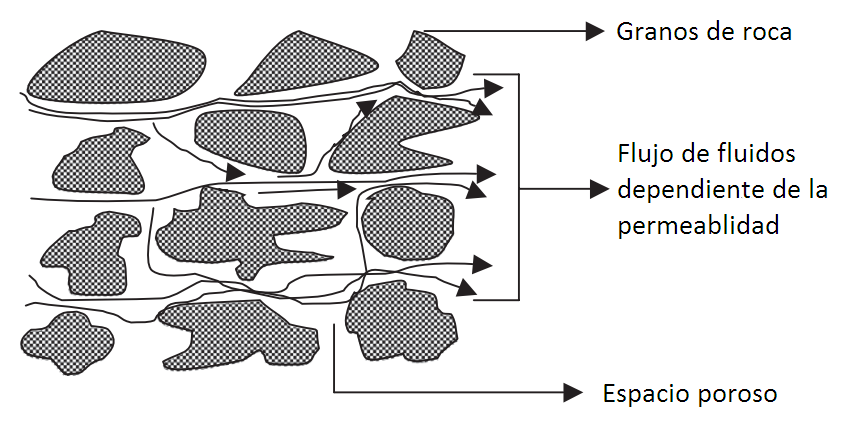
\includegraphics[width=0.9\textwidth]{Graphics/perme1.png}
    \caption[Concepto de Permeabilidad]{Representación conceptual de la permeabilidad de una roca. Adaptado de (\cite{Dandekar}). }
    \label{fig:perme1}
\end{figure}

Esta propiedad ha sido definida de varias maneras por diversos autores (\cite{Dandekar}) como:

\begin{itemize}
    \item La medida de la capacidad de flujo de una roca 
    \item La medida de la capacidad de flujo del medio poroso para transmitir fluidos
    \item La medida de la conductividad de fluido de un medio poroso particular.
    \item La facilidad para fluir o transmitir fluidos a través de una roca que se encuentra completamente saturada con una sola fase de fluido.
    \item La medida del recíproco de la resistencia que el medio poroso ejerce al flujo de un fluido.
    \item La constante de proporcionalidad entre el gasto de flujo de un fluido y el gradiente de presión aplicado.
\end{itemize}


La expresión matemática que define a la permeabilidad fue propuesta por Darcy (cite DARCY) mientras estudiaba el flujo de agua a través de filtros de arena para su purificación, el experimento se muestra en la \autoref{fig:perme2} y cuya única diferencia es la orientación pues el experimento original se llevaba a cabo de manera vertical. 

\begin{figure}
    \centering
    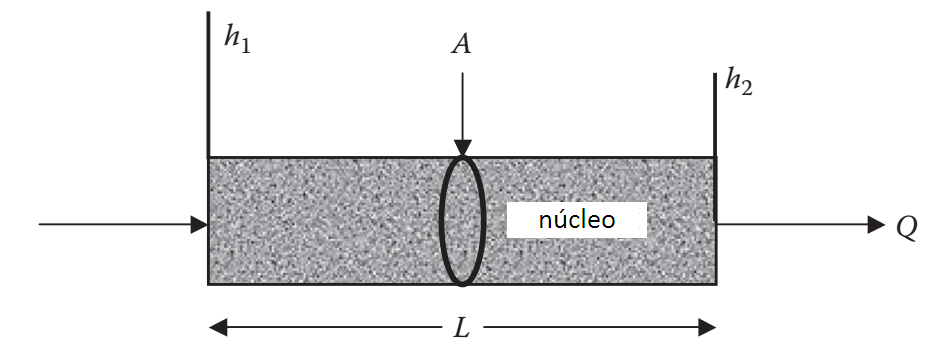
\includegraphics[width=\textwidth]{Graphics/perme2.png}
    \caption[Experimenmto de Darcy]{Experimento de Darcy representando el flujo de un fluido a través de un núcleo de roca . Adaptado de (\cite{Dandekar}). }
    \label{fig:perme2}
\end{figure}

\begin{equation}
Q = KA\frac{h_{1}-h_{2}}{L}
\end{equation}

Donde Q representa el gasto volumétrico a través del núcleo (en $m^{3}/s$ o $ft^{3}/s$), K es la constante de proporcionalidad también definida como conductividad hidráulica (en m/s o ft/s), A es el área transversal del núcleo (en $m^{2}$ o $ft^{2}$), L la longitud del núcleo (en m o ft), y $h_{1}$ y $h_{2}$ representan la carga hidráulica a la entrada y la salida respectivamente (en m o ft).

La ecuación (2) puede ser expresada en término del gradiente de presión d\textit{P} sobre una sección d\textit{L} como:

\begin{gather}
    Q=-KA\frac{dP}{dL}
    \shortintertext{donde}
    dP = \Delta h \rho g
\end{gather}

\textit{d}P es la diferencia entre las presiones corriente arriba y corriente abajo (en $N/m^{2}$), $\Delta h$ es la diferencia entre los gradientes hidráulicos corriente arriba y corriente abajo (m), $\rho$ es la densidad del fluido ($kg/m^{3}$) y g es la aceleración debido a la gravedad ($9.81~m/s^{2}$).
Investigaciones posteriores encontraron que la ley de Darcy puede ser extendida a otros fluidos diferentes al agua, incorporando el término de viscosidad ($\mu$), de manera que la conductividad hidráulica K es expresada como el cociente $k/\mu$, donde k es la \emph{permeabilidad} del medio poroso, lo que permite reescribir la ecuación (3) como:

\begin{equation}
    Q=-\frac{k}{\mu}A\frac{dP}{dL}
\end{equation}
La ecuación (5) puede ser integrada entre los límites de longitud de $0$ a L y de presión a la entrada $P_{1}$ y a la salida $P_{2}$, para el caso del flujo de un fluido como el de la \autoref{fig:perme2} bajo las siguientes suposiciones.

\begin{itemize}
    \item El núcleo se encuentra saturado al 100\% por el fluido.
    \item El flujo es incompresible.
    \item El flujo es horizontal, es estado estacionario y bajo un régimen laminar.
    \item El flujo a través del medio poroso ocurre bajo un régimen viscoso.
    \item El fluido no interacciona con el medio poroso.
\end{itemize}

\begin{gather}
\frac{Q}{A}\int_{0}^{L}dL=-\frac{k}{\mu}\int_{P_{1}}^{P_{2}}dP \\[10pt]
\frac{Q}{A}(L-0) = -\frac{k}{\mu}(P_{2}-P_{1})\\[10pt]
Q=\frac{kA}{\mu L}(P_{1}-P_{2})~~o~~Q=\frac{kA\Delta P}{\mu L}
\end{gather}

La ecuación (8) es comúnmente conocida como la \emph{Ley de Darcy} y se usa extensivamente en cálculos de ingeniería de yacimientos para determinar la permeabilidad absoluta de una roca dentro de un yacimiento. La ecuación (8) representa una combinación de:

\begin{itemize}
    \item La propiedad del medio poroso o la roca de yacimiento esta representado por la permeabilidad k.
    \item La propiedad del fluido esta representado por la viscosidad $\mu$.
    \item La geometría del medio poroso esta representada por el efecto combinado del cociente de su área transversal y longitud A/L.
    \item Las características del flujo están representadas por el gasto Q, y la diferencia de presiones a la entrada y salida $\Delta$P.
\end{itemize}

Aunque las unidades de la permeabilidad en el sistema internacional son de $m^{2}$, la industria petrolera ha adoptado la unidad \emph{darcy} para la permeabilidad en honor del pionero francés. Un medio poroso se dice que posee un darcy de permeabilidad cuando una sola fase de fluido con una viscosidad de $1$ centipoise (cP) satura completamente al medio poroso y fluye a través de este con un gasto de $1cm^{3}/s$ bajo un régimen viscoso y con un gradiente de presión de $1$ atm/cm  en un área transversal de $1cm^{2}$.

\begin{equation}
1~darcy = 1D = \frac{(cm^{3}/s)(cP)}{(cm^{2})(atm/cm)}
\end{equation}

Entre los factores que afectan la permeabilidad absoluta de una roca, encontramos como primer factor el tamaño de grano y la forma. En la \autoref{fig:perme34} (\textbf{a}) se esquematiza un medio poroso hipotético con granos del mismo tamaño y forma en un arreglo uniforme, la figura claramente hace notar que las permeabilidades horizontal y vertical son casi iguales ($k_{H} \approx k_{V}$), dado que sin importar la dirección, las lineas de flujo son similares. Sin embargo al mirar el inciso \textbf{(b)} es obvio que la permeabilidad horizontal es mayor que la vertical, ya que la primera posee lineas de flujo que no presentan restricción al fluido, mientras que en la permeabilidad horizontal las lineas de flujo son tortuosas y significan una mayor restricción.

\begin{figure} \centering
    \subfloat[]{
        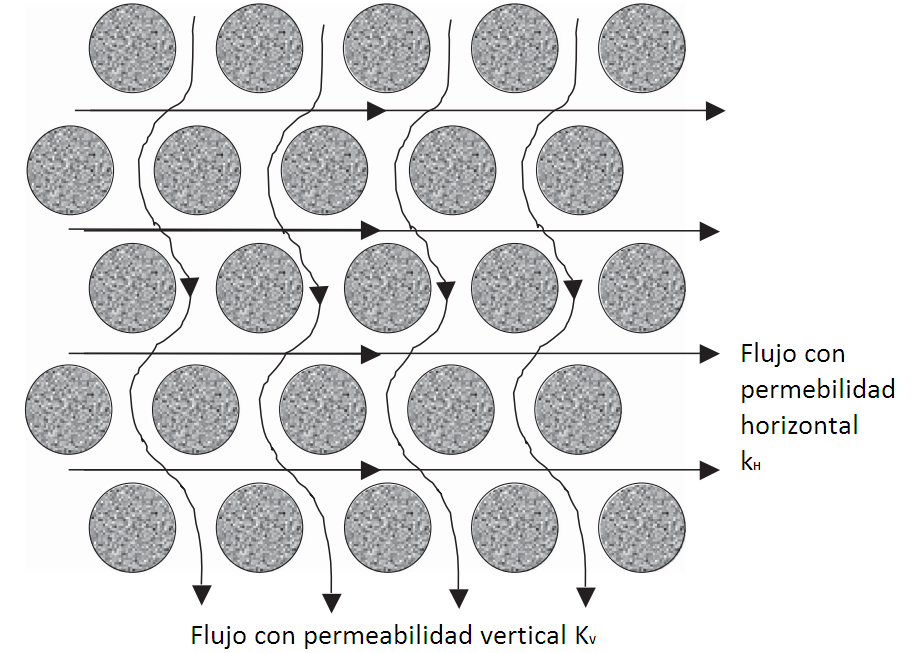
\includegraphics[width=0.8\textwidth]{Graphics/perme3.png} } \quad
    \subfloat[]{
        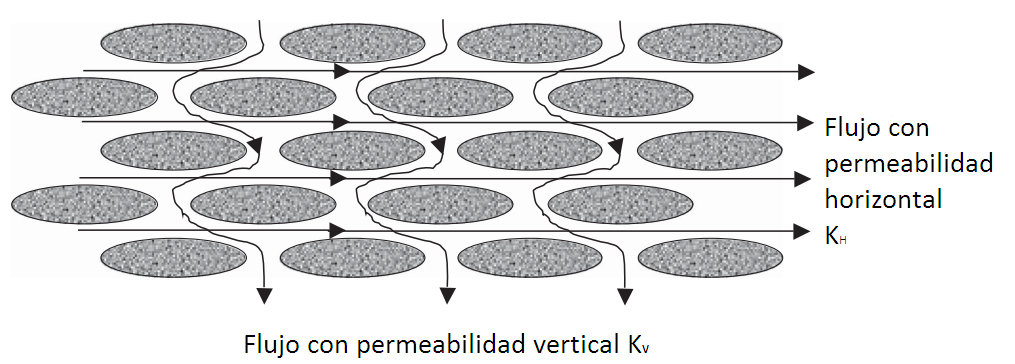
\includegraphics[width=\textwidth]{Graphics/perme4.png} }
    \caption[Permeabilidad vertical y horizontal]{Representación de un medio poroso hipotético formado por: \textbf{(a)} granos de igual tamaño y forma, en un arreglo uniforme ($k_{H}\approx k_{V}$); \textbf{(b)} granos de igual forma aplanados a lo largo en un arreglo uniforme ($k_{H} > k_{V}$). Adaptada de (\cite{Dandekar}).}
    \label{fig:perme34}
\end{figure}

De la misma manera que la porosidad es clasificada en primaria y secundaria, la permeabilidad referida a la matriz cementada de una roca es llamada permeabilidad primaria, mientras que la permeabilidad debido a la presencia de fracturas y canales es conocida como permeabilidad de la fractura o secundaria. En la \autoref{tab:perme1} se muestran las permeabilidades de diferentes tipos de yacimientos alrededor del mundo.

\begin{table}
    \caption[Permebalidades de yacimientos]{Datos de porosidad y permeabilidad de algunas formaciones de arenas y carbonatos alrededor del mundo. Adaptada de (\cite{Dandekar}).}
    \centering \footnotesize
    \begin{tabulary}{\textwidth \tymin=47pt }{L L L L}
        \toprule 
        Campo/Formación & Tipo de Roca &  Porosidad (\%) & Permeabilidad (mD)\\ 
        \midrule              
        Prudhoe Bay, USA & Arena & $22$ & $265$ \\
        Ghawar, Arabia Saudita & Carbonato & $19$ & $617$\\
        Bombay High, India & Carbonato & $15-20$ & $100-250$\\
        Ford Geraldin Unit, USA & Arena  & $23$ & $64$\\
        Elk Hills, USA & Arena & $27-35$ & $100-2000$\\
        Pullai Field, Malasia & Arena & $18-31$ & $300-3000$\\
        Chicontepec, México & Arena & $5-25$ & $0.1-900$\\
        Ekofisk, Noruega & Carbonato  & $30-48$  & $0.25$ \\
        Cretácico superior e inferior, Dinamarca & Carbonato & $15-45$ & $0.01-10$\\
        Daqing, China & Arena & $24.6-26.4$ & $200-1300$\\
        Hassi Messaoud, Algeria & Arena & $7.4$ & $2.5$ \\
        \midrule
        \bottomrule
    \end{tabulary}
    \label{tab:perme1}
\end{table}


\subsection{Saturación}
Mientras que la porosidad representa el la máxima capacidad de una roca para alojar fluidos, la saturación del espacio poroso, cuantifica cuanta de esa capacidad de almacenamiento está realmente ocupada por alguna fase fluida, es decir como se encuentra distribuida o repartida esa capacidad entre las tres fases de fluidos de un yacimiento: agua aceite y gas. Las saturaciones iniciales de fluido, que se definen como las fracciones del espacio poroso ocupado por gas aceite y agua de formación (ecuaciones (10-12)), son los factores clave para determinar la cantidad de hidrocarburos en el yacimiento.
 
 \begin{gather}
    S_{g}=\frac{volumen~ de~ gas}{volumen~ de~ poros}\\[10pt]
    S_{o}=\frac{volumen~ de~ aceite}{volumen~ de~ poros}\\[10pt]
    S_{w}=\frac{volumen~ de~ agua}{volumen~ de~ poros}\\[20pt]
    S_{g}+S_{o}+S_{w}=1.0
 \end{gather}
Donde $S_{g}$, $S_{o}$ y $S_{w}$ son las saturaciones de gas, aceite y agua expresadas en porcentaje o fracción respectivamente. Siempre debe cumplirse que la suma de los volúmenes saturados de alguna fase es igual al total del volumen de poros de la roca ecuación (13). Adicionalmente existen tres casos especiales de saturación de fluidos, que juegan un papel importante para entender el flujo multifásico de fluidos en medios porosos.

\subsubsection{Saturación de gas crítica}
Partiendo del hecho de que los yacimientos de hidrocarburos existen en condiciones de presión y temperatura elevadas y que normalmente el gas hidrocarburo se encuentra disuelto en la fase líquida. Luego de iniciada la producción del yacimiento, la presión de este comienza a declinar mientras la temperatura permanece constante, este cambio en la presión tiene como consecuencia la evolución de una fase gaseosa (la saturación de gas comienza a aumentar desde cero) cuando la presión alcanza un cierto límite de solubilidad conocido como la \emph{presión de saturación} o \emph{punto de burbuja}. La saturación de la fase gas sigue incrementándose mientras que la presión del yacimiento sigue declinando, sin embargo permanece inmóvil o atrapada, hasta que la saturación excede un cierto límite conocido como \emph{saturación de gas crítica} ($S_{gc}$). La fase gaseosa entonces comienza a moverse por encima de esta saturación de gas crítica. Este fenómeno es atribuido al proceso mediante el cual la fase gaseosa se hace continua a través del sistema para comenzar a moverse (\autoref{fig:satgas}).

\begin{figure}\centering
    \subfloat[$S_{g}=0$]{
        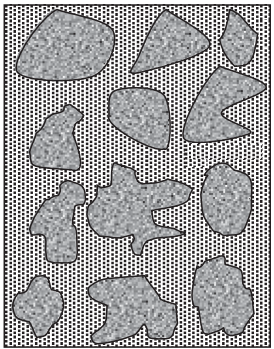
\includegraphics[width=0.3\textwidth]{Graphics/satgasa.png} } \quad
    \subfloat[$S_{g}>0$]{
        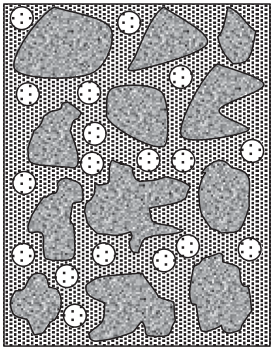
\includegraphics[width=0.3\textwidth]{Graphics/satgasb.png} } \\
    \subfloat[$S_{g} < S_{gc} $]{
        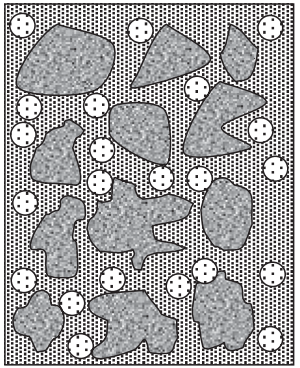
\includegraphics[width=0.3\textwidth]{Graphics/satgasc.png} } \quad
    \subfloat[$S_{g} \ge S_{gc}$]{
        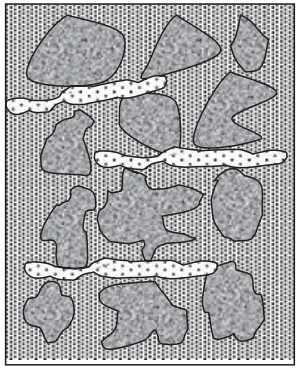
\includegraphics[width=0.3\textwidth]{Graphics/satgasd.png} } \\
    \caption[Saturación de gas crítica]{Representación de los eventos que llevan a la fase gaseosa a la saturación crítica de gas. Adaptada de (\cite{Dandekar})}
    \label{fig:satgas}
\end{figure}

\subsubsection{Saturación residual de aceite}
Esta saturación ($S_{or}$) refiere al aceite remanente en el espacio poroso después de un proceso de desplazamiento. Esta puede ser la saturación de aceite remanente en el yacimiento luego de concluida la explotación primaria. También puede referirse a la saturación de aceite al final de un proceso de recuperación por desplazamiento con gas o agua. Esta saturación también puede ser obtenida en laboratorio en núcleos de roca mediante un proceso de desplazamiento con gas o agua.

\subsubsection{Saturación de agua irreductible}
Los términos \emph{saturación de agua congénita}, \emph{saturación de agua crítica} y \emph{saturación de agua irreductible}, ($S_{wi}$) se encuentran frecuentemente intercambiados en la literatura para hacer referencia al valor de la saturación de agua, al cual la fase agua permanece inmóvil. 

En la mayoría de los yacimientos, los fluidos contenidos han alcanzado un estado de equilibrio, por lo que se han segregado en su mayoría de acuerdo a sus densidades, esto es, gas encima del aceite y este por encima del agua. Se da por hecho que la roca almacenadora se encontraba inicialmente saturada de agua, antes de la migración y entrampamiento de los hidrocarburos (cita). Dado que existe una oposición entre las fuerzas capilares y gravitacionales, la segregación entre las fases no se completa y la saturación de agua se encuentra distribuida a lo largo de las zonas de gas y aceite como se muestra en la \autoref{fig:satagua1}. En estas zonas la saturación de agua se reduce hasta un mínimo, que es la saturación irreductible $Sw_{i}$.
Las fuerzas que retienen esta agua en las zonas de gas y aceite son conocidas como fuerzas capilares y son de importancia debido al tamaño capilar de los poros en la roca. La saturación irreductible de agua depende tanto de la permeabilidad, litología y altura sobre el nivel de la zona invadida por agua, por lo que no se encuentra uniformemente distribuida en el yacimiento.

\begin{figure}
    \centering
    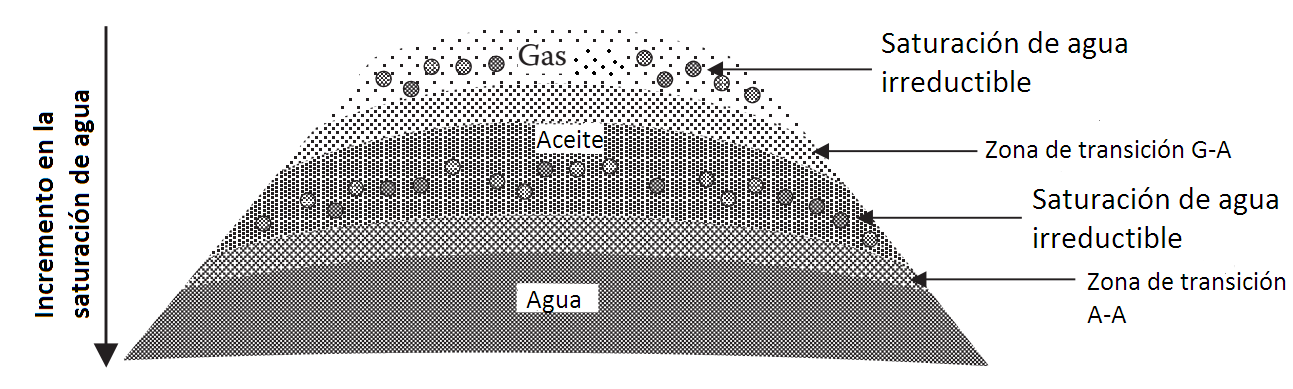
\includegraphics[width=\textwidth]{Graphics/satagua1.png}
    \caption[Saturación de agua irredcutible]{Representación de la saturación de agua irreductible en un yacimiento hipotético. Adaptada de (\cite{Dandekar}). }
    \label{fig:satagua1}
\end{figure}

\subsection{Tensión interfacial}

Para definir este concepto hay que considerar un sistema formado por dos fluidos inmiscibles, agua y aceite (\autoref{fig:tension1}). Una molécula de agua o aceite que se encuentra en el seno del fluido, lejos de la interfase, se encuentra rodeada por otras moléculas de aceite o agua, de esta manera la fuerza de atracción resultante sobre la molécula es igual a cero dado que es \emph{arrastrada} en todas las direcciones. En contraste una molécula en la interfase presenta, tanto una fuerza de atracción ejercida por las moléculas de aceite por encima de la interfase, como atracción por parte de las moléculas de agua bajo esta. Las fuerzas resultantes no están balanceadas debido a que las magnitud de las fuerzas en cada lado de la interfase (arriba y abajo) son distintas, y esto da origen la tensión interfacial.
\begin{description}
    \item[Definición] La tensión interfacial ($\sigma$) es una medida de la energía específica de superficie entre dos fases inmiscibles de diferente composición. Dicho de otra manera es la medida de la energía requerida para formar una unidad de área de interfase entre dos fluidos inmiscibles.
\end{description}
La tensión interfacial tiene dimensiones de fuerza por unidad de longitud expresadas comúnmente en mN/m o $10^{-3}$N/m (dyna/cm).
\begin{figure}
    \centering
    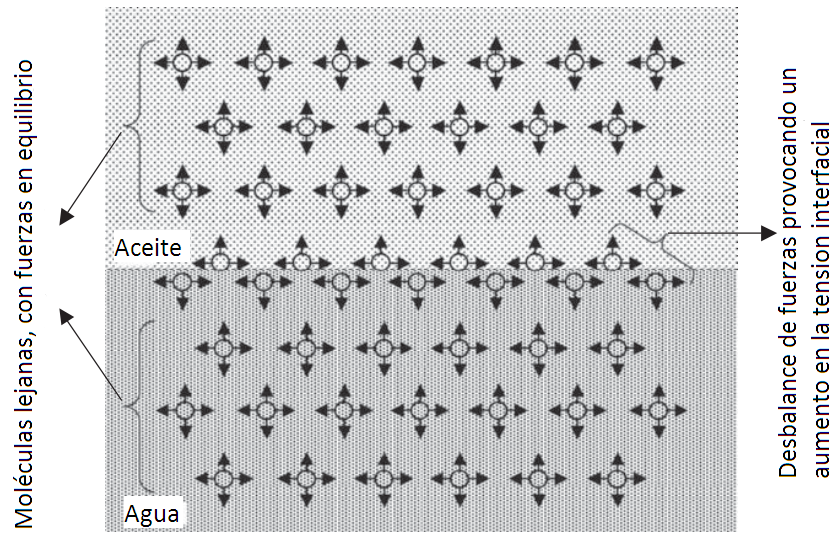
\includegraphics[width=0.8\textwidth]{Graphics/tension1.png}
    \caption[Tensión interfacial]{Representación del concepto de tensión interfacial. Adaptada de (\cite{Dandekar}).}
    \label{fig:tension1}
\end{figure}

\subsubsection{Medición de la tensión interfacial mediante gota pendiente}
Existen diversas técnicas para medir la tensión interfacial, sus características y cualidades se pueden encontrar descritas en el trabajo de \cite{Drelich2002}. El método de la gota pendiente es por mucho el mas simple en términos de instrumentación y versátil. El sistema experimental para medir tensión interfacial por el método de la gota pendiente se compone básicamente por una cámara, una fuente de luz y una aguja (\autoref{fig:dropsystem}).
\begin{figure}
    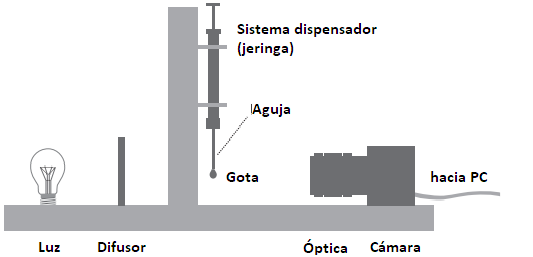
\includegraphics[width=0.8\textwidth]{Graphics/dropsystem.png}
    \caption[Sistema de medicion IFT]{Esquema que muestra el sistema experimental básico para la medición de tensión interfacial por el método de la gota pendiente. Adaptada de (\cite{Berry2015}).}
    \label{fig:dropsystem}
\end{figure}
\subsubsection{Teoría}
Si una gota de líquido se encuentra colgando de la aguja de una jeringa, entonces se asume que tendrá una forma característica de la cual se puede determinar su tensión superficial. La fuerza de gravedad que actúa sobre la gota, dependiendo de su altura, equilibran la presión de Laplace la cual está esta determinada por la curvatura del contorno de la gota. La presión de Laplace está definida en la siguiente expresión conocida como la ecuación de Young-Laplace:
\begin{equation}
\Delta p = \sigma \left( \frac{1}{r_{1}} + \frac{1}{r_{2}} \right)
\end{equation}
Esta expresión describe la diferencia de presión entre el interior y el exterior de una gota que posee como principales radios de curvatura a $r_{1}$ y $r_{2}$. Si la fuerza de gravedad es la única fuerza adicional que actúa sobre la gota, el cambio en la presión puede definirse como $\Delta P = \Delta P_{0}+\Delta \rho gz$, donde $\Delta \rho$ es la diferencia de densidad entre la fases. Utilizando un cambio en el sistema de coordenadas cilíndricas representado en la \autoref{fig:drop}, la ecuación de Young-Laplace se convierte en un sistema de tres ecuaciones diferenciales ordinarias en términos de la longitud de arco $s$ medido desde el apéndice de la gota,
\begin{figure}\centering
    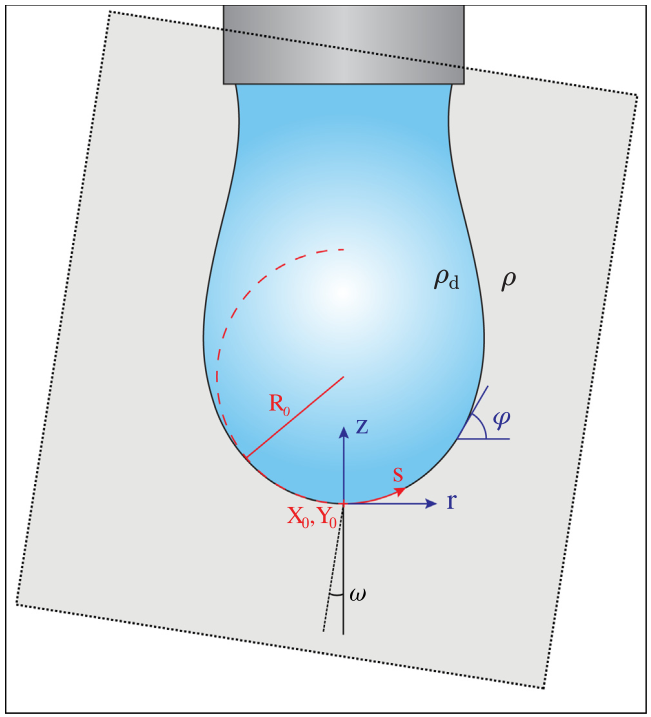
\includegraphics[width=0.6\textwidth]{Graphics/Pendant_drop.png}
    \caption{Esquema de una gota pendiente de una aguja de jeringa, la región sombreada representa el área de imagen capturada por la cámara que no necesariamente se encuentra alineada perfectamente con la gota. Adaptada de (\cite{Berry2015}).}
    \label{fig:drop}
\end{figure}
\begin{eqnarray}
\frac{d\psi}{d\bar{s}} & = & 2-Bo*\bar{z}-\frac{sin(\psi)}{\bar{r}}\\
\frac{d\bar{r}}{d\bar{s}} & = & cos(\psi) \\
\frac{d\bar{z}}{d\bar{s}} & = & sin(\psi)
\end{eqnarray}
la línea indica que se trata de cantidades adimensionales escaladas por $R_{0}$, que es el radio de curvatura en el apéndice de la gota. \emph{Bo} en la ecuación (15) se refiere al número de Bond (\autoref{eqn:bond}).
\begin{equation}
Bo \simeq \frac{\Delta \rho g R_{0}^{2}}{\sigma}
\label{eqn:bond}
\end{equation}
Si el número de Bond asociado con la gota pendiente puede ser determinado junto con el radio de la gota $R_{0}$ en el apéndice, la tensión interfacial $\sigma$ puede obtenerse con la ecuación ($18$). Las condiciones de frontera asociadas son 
\begin{equation}
\bar{r}=0 ,~~ \bar{z}=0,~~ \psi=0 ~~~con~~~ \bar{s}=0
\end{equation}

\subsection{Mojabilidad}%
Dentro de un yacimiento es necesario tomar en consideración las fuerzas que se encuentran activas en la interfase entre líquidos y sólidos, dado que los fluidos de producción, se encuentran necesariamente en contacto con la superficie de la roca. La mojabilidad es un parámetro que determina algunas propiedades del yacimiento como la distribución de aceite agua y gas dentro del yacimiento así como la permeabilidad relativa y la presión capilar.

\begin{description}
    \item[Definición] La mojabilidad es la habilidad de un fluido de esparcirse sobre una superficie sólida en presencia de otro fluido.
\end{description}

Si consideramos la definición anterior, sabemos que la mojabilidad posee un carácter multifásico, dado que se necesitan al menos dos fluidos, con uno de ellos presentando una mayor afinidad hacia la superficie sólida con la que hacen contacto ambos.

La tendencia de un fluido a esparcirse puede ser expresada en términos de la \emph{tensión de adhesión} ($A_{T}$) . La tensión de adhesión es una función de la tensión interfacial y determina la tendencia de mojabilidad de un sistema roca-fluido. Para un sistema de dos fluidos inmiscibles en contacto con una superficie mineral (\autoref{fig:moja1}) la tensión de adhesión se define como:

\begin{figure}
    \centering
    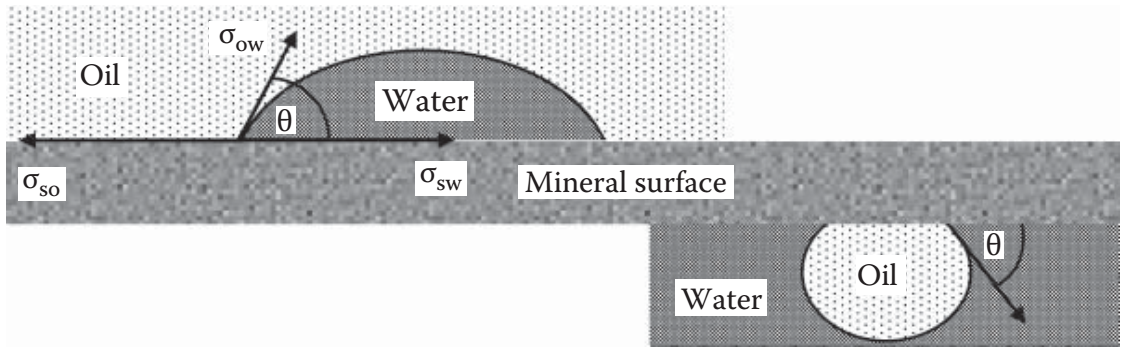
\includegraphics[width=0.9\textwidth]{Graphics/moja1.png}
    \caption[Mojabilidad]{Representación de un sistema de dos líquidos inmiscibles (aceite y agua) en contacto con una superficie mineral. Adaptada de (\cite{Dandekar}).}
    \label{fig:moja1}
\end{figure}

\begin{equation}
A_{T}=\sigma_{SO}-\sigma_{SW}
\end{equation}
Donde $\sigma_{SO}$ es la tensión interfacial entre el sólido y la fase fluida mas ligera (aceite para el caso mostrado) y $\sigma_{SW}$ la tensión interfacial entre el sólido y la fase mas densa (agua para el caso mostrado).

El ángulo de contacto $\theta$ puede varias de $0\degree$ a $180\degree$. Por definición el coseno del ángulo $\theta$ es:

\begin{equation}
cos(\theta_{OW})= \frac{\sigma_{SO}-\sigma_{SW}}{\sigma_{OW}}
\end{equation}

Combinando las ecuaciones (14) y (15):

\begin{equation}
A_{T}=\sigma_{OW}~cos(\theta_{OW})
\end{equation}

Para determinar la tensión de adhesión y definir la mojabilidad del sistema roca-fluido
es necesario conocer el valor de la tensión interfacial entre agua-aceite, y la medida del ángulo de contacto. Un valor de tensión de adhesión positivo indica que la fase mas densa moja preferentemente a la superficie sólida, mientras que un valor negativo indica una preferencia de la fase menos densa a mojar la superficie mineral.

\subsection{Presión capilar}%
La presión capilar existe en un yacimiento siempre que sus poros (de tamaño capilar) se encuentren saturados de dos o más fases inmiscibles fluidas. La frontera entre dos fases inmiscibles presentes en un medio poroso presenta una cierta curvatura debido a la tensión interfacial entre ambos fluidos (\cite{Leverett}). La forma de la curvatura depende de las propiedades de los fluidos y el tamaño de los poros. Es la forma de la curvatura en la interfase lo que da lugar a una diferencia de presión de un lado a otro de la interfase, llamada \emph{presión capilar} ($P_{c}$). Esto significa que cada uno de los fluidos inmiscibles tiene una presión que es distinta de la del otro. 

La presión en la fase no mojante es mayor con respecto de la presión en la fase mojante y por tanto la interfase es curva y convexa respecto a la fase no mojante. Lo anterior puede expresarse de la siguiente manera:

\begin{gather*}
\begin{gathered}
presion~capilar~ = ~presion~fase~no~mojante \\ - ~presion~fase~mojante
\end{gathered} \\
P_{c}=P_{nw}-P_{w}
\end{gather*}


Basado en la altura de líquidos dentro de tubos capilares (\cite{Amix}) desarrolló una serie de ecuaciones que describen la presión capilar en función de la tensión interfacial, el tamaño de poro y la mojabilidad. Si miramos el esquema de la \autoref{fig:capilar1} podemos plantear un balance de fuerzas, dado que el sistema se encuentra en equilibrio, para relacionar la altura del fluido dentro del capilar con el radio, la diferencia de densidades entre el aire y el líquido y la aceleración de la gravedad:

\begin{figure}
    \centering
    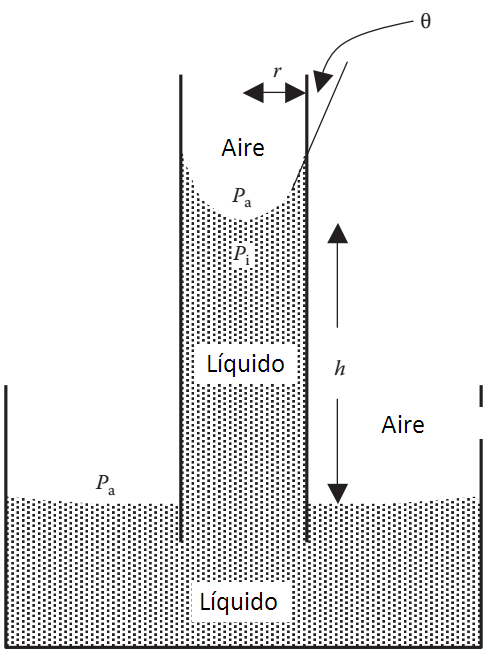
\includegraphics[width=0.6\textwidth]{Graphics/capilar1.png}
    \caption[Presión Capilar]{Esquema que representa las relaciones entre las presiones dentro de un tubo capilar. Adaptada de (\cite{Dandekar}).}
    \label{fig:capilar1}
\end{figure}

\begin{gather}
Fuerza~arriba=2\pi rA_{T} \\[10pt]
Fuerza~abajo=\pi r^{2} h (\rho_{l}-\rho_{a}) g
\end{gather}

Donde $A_{T}$ es la tensión de adhesión (N/m), r es el radio del tubo capilar (m), h es la altura del fluido en el capilar (m), $\rho_{l}$ y $\rho_{a}$ son las densidades del líquido y del aire respectivamente (Kg/$m^{3}$) y g es la aceleración de la gravedad (m/$s^{2}$).

\begin{gather}
2\pi r A_{T} = \pi r^{2} h (\rho_{l}-\rho_{a}) g \\[10pt]
h= \frac{2\pi r A_{T}}{\pi r^{2}(\rho_{l}-\rho_{a}) g}=\frac{2 A_{T}}{r (\rho_{l}-\rho_{a}) g}
\end{gather}

Sin embargo si consideramos la definición de tensión de adhesión, $A_{T} = \sigma_{al}~cos(\theta_{al})$; entonces

\begin{equation}
h=\frac{2 \sigma_{al}~cos(\theta_{al})}{r(\rho_{l}-\rho_{a})g}
\end{equation}

Ahora por definición de presión capilar, una diferencia de presión existe de la interfase líquido aire y puede expresarse como:

\begin{equation}
P_{c}=P_{a}-P_{l}=(\rho_{l}-\rho_{a})gh
\end{equation}

Si combinamos las ecuaciones (23) y (24) obtenemos la ecuación de la presión capilar en términos de las fuerzas de superficie, mojabilidad y tamaño capilar:

\begin{equation}
P_{c} = (\rho_{l}-\rho_{a}) g \frac{2 \sigma_{al}~cos(\theta_{al})}{r(\rho_{l}-\rho_{a}) g} = \frac{2 \sigma_{al} cos~(\theta_{al})}{r}
\end{equation}

De manera general las fuerzas capilares en un yacimiento son la manifestación del efecto de la tensión interfacial, mojabilidad y tamaño de poro del sistema roca-fluido. Las fuerzas capilares son las causantes del entrampamiento de los hidrocarburos en la roca. Un yacimiento antes de la explotación se encuentra en equilibrio capilar-gravitacional. Este equilibrio se manifiesta por medio de una distribución de la saturación de fluidos particular de cada sistema. Por ejemplo en la migración de los hidrocarburos hacia una formación saturada por agua (acuífero) el petróleo entrampado en el yacimiento representa un equilibrio entre la gravedad que intenta moverlo hacia arriba y las presiones capilares que se oponen (\cite{Leverett}). 

Las fuerzas capilares juegan un papel importante en el flujo de dos fluidos inmiscibles en un medio poroso, puesto que la presión capilar debe ser vencida para que una burbuja de aceite o gas pueda fluir a través del pequeño diámetro de un poro. Por ejemplo se necesitan mas de $1480$ psi para hacer fluir una gota esférica de aceite a través de un diámetro de poro de $0.01~\mu$m, asumiendo que la roca se encuentra saturada por agua y que la tensión interfacial agua-aceite es de $25~\mu$N/m.


\subsection{Permeabilidad Relativa}%

Para extender la ley de Darcy al flujo simultaneo de dos o mas fluidos en un medio poroso, es necesario incluir el concepto de \emph{permeabilidad efectiva} de cada fase, en lugar de la permeabilidad absoluta definida anteriormente. La permeabilidad efectiva es función de la saturación de fluido, las características de mojabilidad del medio y de la geometría de los poros. Por lo anterior es necesario además, especificar la saturación del fluido para definir su permeabilidad efectiva. Dada la gran cantidad de combinaciones de saturaciones de dos o más fluidos dentro de un medio poroso, los datos de permeabilidad son reportados como \emph{permeabilidad relativa} ($K_{r}$) en lugar de permeabilidad efectiva \autoref{fig:satrel}.

\begin{figure}
    \centering
    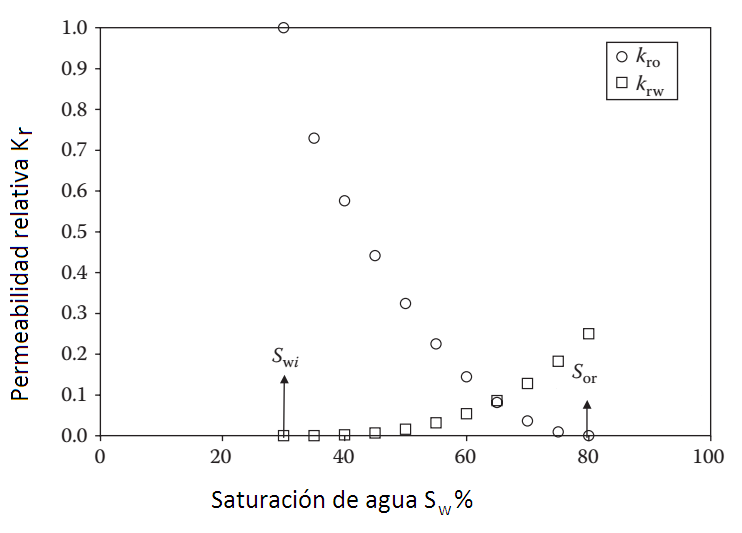
\includegraphics[width=0.8\textwidth]{Graphics/satrel.png}
    \caption[Saturación relativa]{Curva típica de saturación relativa para agua y aceite. Adaptada de \cite{Dandekar}.}
    \label{fig:satrel}
\end{figure}

\begin{description}
    \item[Definición]La permeabilidad relativa se refiere a la proporción entre la permeabilidad efectiva de un fluido con respecto de la permeabilidad absoluta del medio (ecuación (24)). La permeabilidad relativa es una medida de la conductividad de un fluido en el medio poroso, cuando este se encuentra saturado con otros fluidos (\cite{Dandekar}). 
\end{description}

\begin{equation}
K_{r}=\frac{K_{e}}{K}
\end{equation}

Donde $k_{r}$ es la permeabilidad relativa (adimensional) y $K_{e}$ es la permeabilidad efectiva (mD o D).
La ecuación anterior puede ser escrita para cada una de las fases aceite gas y agua:

\begin{gather}
K_{rg}=\frac{K_{eg}}{K} \\
K_{ro}=\frac{K_{eo}}{K} \\
K_{rw}=\frac{K_{ew}}{K}
\end{gather}

%\chapter{Surfactantes}
\label{chp:tensoactivos}

\section{Introducción}
En el momento en que consideramos una dispersión fina de una fase dentro de otra, la interfase que delimita cada una de ellas se convierte en un tema de importancia. Esta relación se genera de manera natural debido a que la materia particulada posee una proporción mucho mayor de área superficial respecto a la masa. En la \autoref{fig:Area} se muestra este concepto, el área superficial de una esfera con radio de $1~cm$ ($4 \pi r^{2}$) es de aproximadamente $12~cm^{2}$, mientras que el área superficial de la misma cantidad de material pero en forma de esferas de diámetro de $1\mu$m es de $120000~cm^{2}$.
%The link between colloids and surfaces follows naturally from the fact %that particulate matter has a high surface area to mass ratio. The %surface area of a 1cm diameter sphere (4pr2) is 3.14cm2, whereas the %surface area of the same amount of material but in the form of 0.1mm %diameter spheres (i.e. the size of the particles in latex paint) is %314000cm2.
\begin{figure}
    \centering
    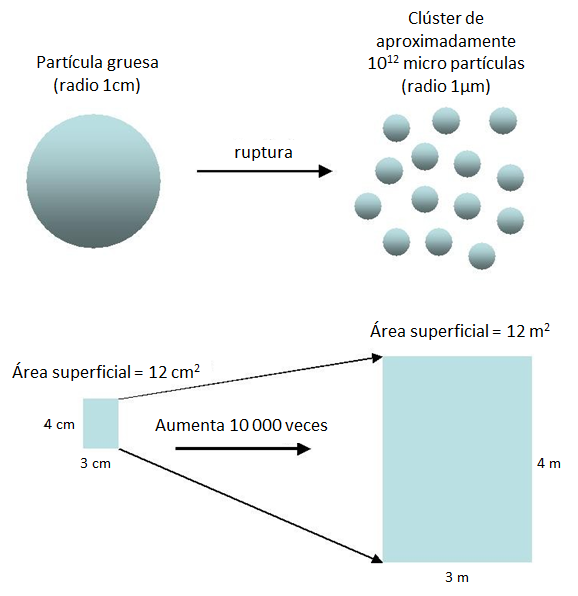
\includegraphics[width=0.7\textwidth]{Graphics/Area.png}
    \caption[Área superficial]{El área superficial de una esfera con radio de $1$cm ($4 \pi r^{2}$) es de aproximadamente $12 cm^{2}$ (como un cuadrilátero de $3 x 4$ cm), el mismo volumen ($4.2 cm^{3}$) puede ser ocupado por $10^{12}$ esferas de radio $1 \mu$m, con un área superficial de $12m^{3}$ (como un cuadrilátero de $3 x 4$ m). }
    \label{fig:Area}
\end{figure}

\subsection{Interfase}

\begin{description}
    \item [Definición] Para que dos fases existan en contacto una con otra, debe haber una región a través de la cual las propiedades intensivas del sistema pasen de las de una fase, a las de otra fase (\cite{Cosgrove}).
\end{description}
    
 Los términos \emph{superficial} e \emph{interfacial} se pueden encontrar intercambiados en la literatura, aunque rigurosamente tienen significados distintos. De manera general se puede decir que el término superficial se aplica en la región entre una fase condensada (líquido o sólido) y una fase gas o vacío, mientras que el término interfacial se aplica a sistemas que involucran dos fases condensadas.
 
 \subsection{Actividad Superficial}
 Algunas sustancias como los ácidos grasos y los alcoholes son solubles tanto en solventes como el agua y el aceite. La parte hidrocarburo de la molécula le concede la solubilidad en aceite, mientras el grupo polar, posee suficiente afinidad al agua, como para arrastrar consigo a una cadena corta de hidrocarburos no polar dentro de una solución acuosa.
 
 Estos materiales están formados de moléculas que cuando son disueltas en un solvente en bajas concentraciones, poseen la habilidad de adsorberse (o localizarse) en la interfase. Este comportamiento de adsorción es atribuido a la naturaleza del solvente y a la estructura química de la sustancia, que poseen un grupo polar y uno no polar en la misma molécula (ambifílicos).
 
 La fuerte adsorción de estos materiales en la interfase (o superficie) para formar una película monomolecular (o monocapa) es denominada como actividad superficial (\cite{Duncan}).
 
 \section{Surfactantes}
 
 Los materiales que presentan actividad superficial son denominados surfactantes o tensoactivos. En general los tensoactivos poseen una estructura química característica (ver \autoref{fig:Tenso}) que consiste de:
 
 \begin{itemize}
     \item Componente molecular de poca afinidad con la fase que lo rodea (por ejemplo el solvente) normalmente llamado el grupo liofóbico.
     \item  Unidades químicas que poseen una fuerte atracción hacia la fase que las rodea, denominadas el grupo liofílico.
 \end{itemize}

\begin{figure}
    \centering
    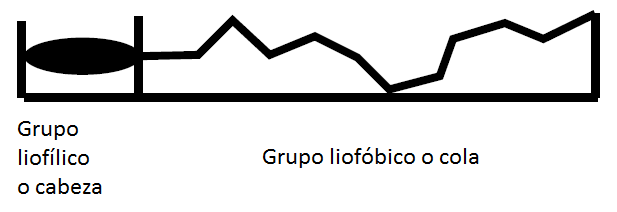
\includegraphics[width=0.9\textwidth]{Graphics/Tenso.png}
    \caption[Estructura de un tensoactivo]{La estructura básica de un material tensoactivo consiste de un grupo liofóbico que posee poca afinidad por el solvente y el grupo liofílico el cual presenta una fuerte interacción con el solvente. Adaptada de (\cite{Drew}). }
    \label{fig:Tenso}
\end{figure}


%Uno de los tipos de sistemas coloidales, clasificados como coloides de asociación (\autoref{chp:antescedentes}), son agregados de moléculas ambifílicas, que se asocian en un proceso impulsado dinámica y termodinámicamente, de manera que pueden ser soluciones a nivel molecular y sistemas coloidales simultáneamente.
%
%Los surfactantes son una importante y versátil clase de químicos. Debido a su naturaleza dual, están asociados con diversos fenómenos superficiales, por ejemplo la mojabilidad, y estos a su vez se encuentran en varios procesos industriales (\cite{Cosgrove}).

\subsection{Características de los surfactantes}

Debido a su naturaleza dual, los surfactantes se sitúan (adsorben) en la interfase de modo que su sección liofóbica (cola) se mantiene alejada de las fuertes interacciones con el solvente, mientras que la parte liofílica (cabeza) permanece en solución (\autoref{fig:adsorb}).

La adsorción esta asociada con un cambio energético dado que la energía libre de una molécula surfactante localizada en la interfase es menor que la de la misma molécula solubilizada en el seno de cualquiera de las fases. La acumulación de ambífilos en la interfase es un proceso espontáneo que resulta en la disminución de la tensión interfacial (o superficial). Este fenómeno ocurre con muchas otras sustancias como algunos alcoholes de media y larga cadena (ejemplo: n-hexanol, duodecanol), estos son sustancias que no son consideradas como surfactantes. 
Un surfactante se distingue por su capacidad de formar capas orientadas de moléculas en la interfase, y mas importante, formar estructuras autoensambladas (miscelas, vesículas) dentro del seno de las fases (\cite{Cosgrove}).

\begin{figure}
    \centering
    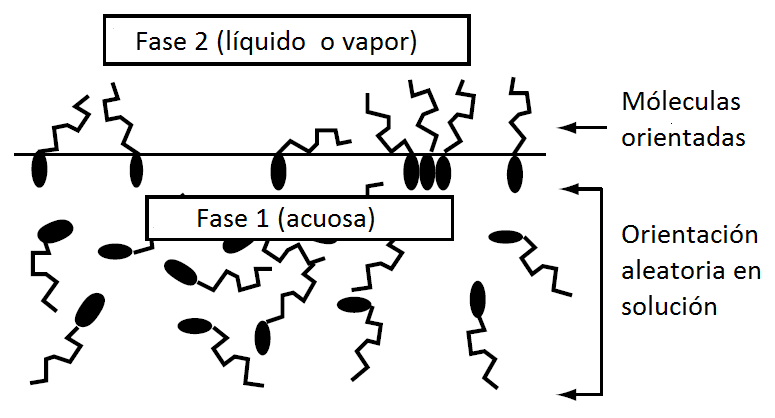
\includegraphics[width=0.9\textwidth]{Graphics/Adsorb.png}
    \caption[Adsorción en la interfase]{Cuando ocurre la adsorción en la interfase, las moléculas adsorbidas tienden a orientarse de manera que minimizan las interacciones no favorables entre la fase acuosa y las secciones de la molécula surfactante. Adaptada de (\cite{Drew}). }
    \label{fig:adsorb}
\end{figure}


\subsection{Clasificación}
Existen numerosas variaciones dentro de la estructura química de los grupos cola y cabeza de la molécula surfactante. El grupo cabeza puede tener carga o ser neutro, puede tratarse de una estructura pequeña y compacta o una cadena polimérica. El grupo cola normalmente es un hidrocarburo lineal o ramificado sencillo o doble, peor también puede ser un fluorocarbonado, un siloxano o contener grupos aromáticos. 

Dado que el solvente mas común e importante para los procesos industriales es el agua, comúnmente se describen a los surfactantes en función de sus grupos  hidrofílicos (cabezas) e hidrofóbicos (colas). Algunos de los grupos hidrofílicos e hidrofóbicos mas comunes se encuentran muestran en la \autoref{tab:surf1} y \autoref{tab:surf2}.

\begin{table}
 \caption[Grupos Hidrofílicos]{\raggedright Grupos hidrofílicos comúnmente encontrados en surfactantes comerciales (\cite{Cosgrove}).}
     \centering \footnotesize
     \begin{tabulary}{\textwidth}{L|L}
     \toprule 
        Clase & Estructura General\\ 
        \midrule              
        Sulfonato & $R-SO_{3^{-}}M^{+}$ \\
        Sulfato & $R-OSO_{3^{-}}M^{+}$ \\
        Carboxilato &  $R-COO^{-}M^{-}$ \\
        Fosfato & $R-OSO_{3^{-}}M^{+} $ \\
        Amonio & $R_{x}H_{y}N^{+}X^{-}$ \{$x=1-3, y=4-x$ \} \\
        Amonio cuaternario & $R_{4}N^{+}X^{-}$\\
        Betainos & $RN^{+}(CH_{3})_{2}CH_{2}COO^{-}$\\
        Sulfobetainos & $RN^{+}(CH_{3})_{2}CH_{2}CH_{2}SO_{3^{-}}$\\
        Polioxietileno & $R-OCH_{2}CH_{2}(OCH_{2}CH_{2})_{n}OH$\\
        Polioles & Sucrosa, sorbitan, glicerol, etilenglicol, etc.\\
        Polipéptidos & $R$-$NH$-$CHR$-$CO$-$NH$-$CHR'$-$CO$-...-$CO_{2}H$\\
        Poliglicidil & $R$-$(OCH_{2}CH[CH_{2}OH]CH_{2})_{n}$- ... -$OCH_{2}CH[CH_{2}OH$\\
     \midrule
     \bottomrule
     \end{tabulary}
     \label{tab:surf1}
\end{table}

\begin{table}
    \caption[Grupos Hidrofóbicos]{\raggedright Grupos hidrofóbicos comúnmente encontrados en surfactantes comerciales (\cite{Cosgrove}).}
    \centering \footnotesize
    \begin{tabulary}{\textwidth \tymin=99.73pt}{|L|L L|}
        \toprule 
        Grupo & Estructura general & ~\\ 
        \midrule              
        Alquilos & $CH_{3}(CH_{2})_{n}$ & n = $12$ - $18$\\
        Olefinas & {\scriptsize $CH_{3}(CH_{2})_{n}CH$=$CH_{2}$} & n = $7$ - $17$ \\
        %\multicolumn{3}{c}{~}\\ %%con esto dejamos una linea vacía
        Alquilbenzenos & \setatomsep{1em}\chemfig{[:0]CH_3{(}CH_2{)}_nCH_2-*6(=-=-=-)} & n = $6-10$, lineal o ramificado\\
        \multicolumn{3}{c}{~}\\ %con esto dejamos una linea vacía
        Alquilaromáticos & ~ & n = $1$ - $2$ soluble en agua ~~~~~ n = $8$ o $9$, soluble en aceite \\
        \multicolumn{3}{c}{~}\\ %con esto dejamos una linea vacía
        Alquilfenoles & \scriptsize\setatomsep{1em}\chemfig{[:0]CH_3{(}CH_2{)}_nCH_2-*6(=-=(-[,1.0]OH)-=-)} & n = $6-10$, lineal o ramificado\\
        \multicolumn{3}{c}{~}\\ %con esto dejamos una linea vacía
        Polioxipropilenos & ~ & n = grado oligomerización ~~~~~~~
        X = iniciador oligomérico \\
        \multicolumn{3}{c}{~}\\ %con esto dejamos una linea vacía
        Fluorocarbonados& $CF_{3}(CF_{2})_{n}COOH$ & n = $4-8$, lineal, ramificado o hidrogenado\\
        Siliconas & {\scriptsize\chemfig{CH_3O{(}SiO{)}_nCH_3}} & ~ \\
        \midrule
        \bottomrule
    \end{tabulary}
    \label{tab:surf2}
\end{table}

La clasificación mas útil para los agentes surfactantes se basa en la naturaleza del hidrófilo y los subgrupos se definen por la naturaleza del hidrófobo (\cite{Drew}). Los cuatro grandes grupos de surfactantes se definen como:

\begin{description}
    \item[Aniónicos] El grupo hidrofílico posee una carga negativa, como en el carboxil, sulfonatos y sulfatos.
    \item[Catiónicos] Con el hidrófilo exhibiendo una carga positiva, como por ejemplo en los haluros de amonio cuaternario.
    \item[No iónicos] Donde el hidrófilo no tiene carga pero debe su solubilidad en agua a grupos altamente polares como azúcares, polioxietileno o grupos similares.
    \item[Zwitteriónicos] También llamados \emph{anfóteros} son aquellos cuya molécula tiene o puede tener, una carga negativa y una positiva en su cadena principal (\autoref{fig:ZW1}).
\end{description}

%En química un zwitterion, palabra que proviene del alemán \textit{zwitter = híbrido}, es una molécula que posee carga positiva y negativa en diferentes puntos dentro de la molécula, pero que su carga neta es cero  (\autoref{fig:ZW1}). Los zwitteriones son llamados también \emph{sales internas}, iones \textit{amfolíticos o amfolitos (amfóteros)} (\cite{Dictionary:chem}). 


\begin{figure}
    \centering
    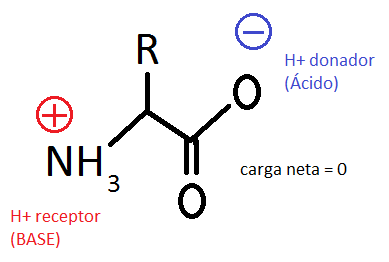
\includegraphics[width=0.7\textwidth]{Graphics/ZW3.png}
    \caption[Molécula zwitterion general]{En química un zwitterion, palabra que proviene del alemán \textit{zwitter = híbrido}, es una molécula que posee carga positiva y negativa en diferentes puntos dentro de la molécula, pero que su carga neta es cero. Los zwitteriones son llamados también \emph{sales internas}, iones \textit{amfolíticos o amfolitos (amfóteros)} (\cite{Dictionary:chem}).}
    \label{fig:ZW1}
\end{figure}

Debido a sus cargas eléctricas, un zwitterion será altamente soluble en agua y también soluble en solventes orgánicos. Las moléculas de agua son polares debido a la diferencia en cargas eléctricas entre las molécula de hidrógeno y oxígeno en el agua; esto es, los átomos de oxígeno del agua son atraídos por los cationes y los átomos de hidrógeno son atraídos por los aniones. Cuando un zwitterion es disuelto en agua, los átomos de hidrógeno rodean de manera inmediata el grupo negativamente cargado de la molécula zwitteriónica mientras que el los átomos de oxigeno del agua rodearan inmediatamente el grupo del zwitterion cargado positivamente, de este modo se logra una completa disolución en agua (\cite{Lenhinger:chem}).

\section{Propiedades de los surfactantes en solución}
Las soluciones de materiales con alta actividad superficial exhiben un comportamiento inusual en sus propiedades físicas. En soluciones diluidas un surfactante actúa como un soluto normal (como electrólito en el caso de un surfactante iónico). Sin embargo en ciertas concentraciones 
se presenta un cambio abrupto en varias propiedades físicas como la conductividad eléctrica, la presión osmótica, la turbidez y le tensión superficial (\autoref{fig:CMC}). El aumento de la presión osmótica con la concentración se vuelve anormalmente bajo y el aumento de la turbidez con la concentración se acelera.

\begin{figure}
    \centering
    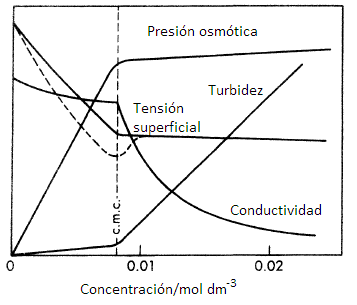
\includegraphics[width=0.9\textwidth]{Graphics/cmc.png}
    \caption[Concentracion micelar crítica]{La gráfica representa el cambio abrupto de las propiedades en la solución surfactante después de la concentración micelar crítica. Adaptada de (\cite{Duncan}). }
    \label{fig:CMC}
\end{figure}



Este comportamiento anómalo puede ser explicado en términos de la formación de agregados o micelas de iones surfactantes en los que las cadenas hidrocarbonadas lipofílicas se orientan hacia el interior de la micela, dejando al grupo hidrofílico en contacto con el medio acuoso (\autoref{fig:micela}) (\cite{McBain}). La concentración a partir de la cual la formación de micelas se vuelve apreciable se denomina \emph{concentración micelar crítica} (c.m.c). La micelación es un mecanismo alterno a la adsorción mediante el cual la energía interfacial de una solución surfactante decrece.

\begin{figure}
    \centering
    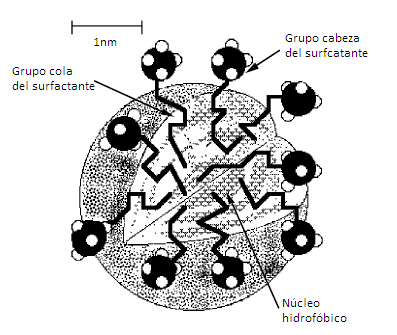
\includegraphics[width=0.9\textwidth]{Graphics/micela.png}
    \caption[Estructura general de una micela]{Representación de la estructura general de una micela. Adaptada de (\cite{Pashley}). }
    \label{fig:micela}
\end{figure}

La concentración micelar crítica puede ser determinada midiendo alguna propiedad física que se vea influenciada por la formación de estas estructuras contra la concentración de surfactante. En la práctica la tensión superficial y la conductividad eléctrica son las mas populares.

\section{Estructuras micelares}

\section{Estructuras supramoleculares}

\begin{description}
%    \item[Definición] En términos generales un gel puede ser definido como un estado intermedio de la materia entre el comportamiento reológico de sólido y el de un líquido. Consiste de una fase dispersa (polímero o coloide) y un medio de dispersión (agua u otro solvente), y puede ser muy semejante a un líquido o a un sólido. Su característica líquida se debe a que el mayor constituyente es el solvente. Su comportamiento de sólido proviene de la red formada por retículos que impide que el gel fluya y se caracteriza por tener un módulo elástico finito \cite{Nishinari2009}.
\item[Retículo] Según la \emph{IUPAC} \cite{IUPAC2} se trata de una región pequeña en un macromolécula en la cual al menos se forman cuatro cadenas formadas por reacciones o grupos de moléculas, o por interacciones entre moléculas existentes. Una región pequeña puede tratarse de un átomo, un grupo de átomos o un número de ramificaciones conectadas por enlaces, grupos de átomos o cadenas oligoméricas. En la mayoría de los casos un retículo es una estructura covalente sin embargo se utiliza también para describir interacciones químicas más débiles e incluso interacciones físicas.
\end{description}


\section{Reología}
\begin{description}
    \item[Reología] La reología es la rama
    \item[Reometría] La reometría es rama de la reología
\end{description}

Para introducir los conceptos básicos de reología hay que considerar un líquido contenido entre dos placas paralelas a cierta distancia \emph{h} como se muestra en la \autoref{fig:reo1}. La placa superior se desliza con una velocidad $v$ in la dirección \emph{x}, mientras que la placa inferior permanece estática. A velocidades suficientemente bajas para evitar la turbulencia, el fluido se moverá de manera uniforme y paralelo a las placas. Las velocidades locales $v_{x}$ varían de manera lineal en el espacio entre placas. En muchos casos las capas de fluido mas cercanas a las placas tienen la misma velocidad que la placa. De esta manera el gradiente $dv_{x}/{dy}$ de $v_{x}$ en la dirección \emph{y} es constante en todo el líquido.

\begin{figure}\centering
    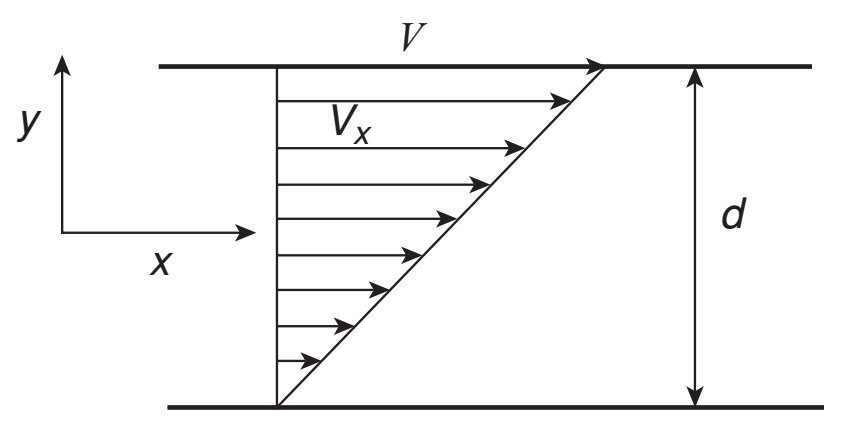
\includegraphics[width=0.7\textwidth]{Graphics/reo1.png}
    \caption[Flujo entre placas]{Flujo cortante entre dos placas, una fija y otra deslizante separadas por una distancia \emph{h}. Adaptada de ().}
    \label{fig:reo1}
\end{figure}

\begin{equation}
\frac{dv_{x}}{dy}= \frac{V}{h}=\dot{\gamma}=constante
\end{equation}

Para generar el flujo se necesita aplicar una fuerza \emph{$F_{xy}$} a la placa superior. El primer subíndice \emph{x} especifica la dirección en la cual se aplica la fuerza mientras el segundo \emph{y}, define el plano al cual se le aplica la fuerza en términos de la normal del plano. La fuerza requerida para mover la placa superior a una velocidad $v$ es proporcional al área superficial de las placas. Por lo anterior, la característica que es relevante en la dinámica involucrada es la fuerza por unidad de área o esfuerzo, $\sigma_{xy}$. Este esfuerzo de corte es trasmitido de una placa a otra y actúa sobre cada elemento del fluido entre ellas. El factor cinético que determina el nivel de los esfuerzos internos, en este caso es el gradiente de velocidad o velocidad de corte. Para fluidos con baja concentración molar, la ecuación constitutiva de Newton para la viscosidad puede ser aplicada. Esta relación especifica, en términos simples, que el esfuerzo es proporcional al gradiente de velocidad. La constante de proporcionalidad, es el coeficiente de viscosidad $\eta$, que expresa la resistencia al flujo para \emph{Fluidos Newtonianos}.

\begin{equation}
\sigma_{xy}=\eta \frac{dv_{x}}{dy}
\end{equation}

La \emph{Ley de Newton} es el ejemplo mas simple de una ecuación constitutiva de reología. Esta expresa la relación intrínseca entre esfuerzos y la cinética para un fluido. Se puede combinar con las leyes de conservación de masa, momento y energía para resolver varios problemas de flujo.

\subsection{Cinemática}
Los flujos no son siempre sencillos como en el caso de la \autoref{fig:reo1}. En términos generales la velocidad no se encuentra necesariamente orientada a lo largo de una linea coordenada. Esta debe ser descrita por un campo de vectores $v$(r) en el cual la velocidad $v$ para cada posición r(x,~y~,z) tiene componentes en las direcciones coordenadas ($v_{x},v_{y},v_{z}$). En la figura anterior solamente una componente de la velocidad diferente de cero varia en solo una dirección coordenada. En general para flujo en tres dimensiones, cualquier gradiente de cualquier componente puede ser diferente de cero. Por lo tanto el gradiente de velocidad debe ser representado por una matriz $\nabla v$:

\begin{equation} 
\nabla v = \left( 
\begin{matrix} 
\delta v_{x}/\delta{x} & \delta v_{x}/\delta{y} & \delta v_{x}/\delta{z} \\
\delta v_{y}/\delta{x} & \delta v_{y}/\delta{y} & \delta v_{y}/\delta{z} \\
\delta v_{z}/\delta{x} & \delta v_{z}/\delta{y} & \delta v_{z}/\delta{z} 
\end{matrix} \right)
\end{equation}

Para el caso de un flujo cortante en una sola dimensión usando coordenadas cartesianas, por convención \emph{x} (ó $1$) es la dirección de flujo, \emph{y} (ó $2$) es la dirección del gradiente, y \emph{z} (ó 3) la dirección neutral o de vorticidad. Las componentes de la matriz en la ecuación (30) representan entidades físicas y por lo tanto obedecen a ciertas reglas de transformación para los componentes o tensores (o transformaciones lineales). Lo mismo aplica para las componentes de esfuerzo.

El vector $v$ y el tensor $\nabla v$ pueden contener componentes diferentes de cero aun cuando no exista el flujo. Este caso, por ejemplo, se presenta cuando un líquido rota como un cuerpo solido sin algún flujo. Lo anterior hace que el gradiente de velocidad no sea adecuado para describir la cinemática en una ecuación constitutiva. Este inconveniente se evita utilizando la parte simétrica del gradiente de velocidad, que no se ve afectada por la rotación como cuerpo sólido. Esto resulta en el tensor de tasa de deformación, \textbf{D}, con componentes:

\begin{equation}\Large
D_{ij} = \left(
\begin{matrix}
%
\frac{\delta v_{x}}{\delta{x}} & \frac{1}{2}(\frac{\delta v_{x}}{\delta{y}}+\frac{\delta v_{y}}{\delta{x}}) & \frac{1}{2}(\frac{\delta v_{x}}{\delta{z}}+\frac{\delta v_{z}}{\delta{x}}) \\
%
\frac{1}{2}(\frac{\delta v_{y}}{\delta{x}}+\frac{\delta v_{x}}{\delta{y}}) & \frac{\delta v_{y}}{\delta{y}} & \frac{1}{2}(\frac{\delta v_{y}}{\delta{z}}+\frac{\delta v_{z}}{\delta{y}}) \\
%
\frac{1}{2}(\frac{\delta v_{z}}{\delta{x}}+\frac{\delta v_{x}}{\delta{z}}) & \frac{1}{2}(\frac{\delta v_{z}}{\delta{y}}+\frac{\delta v_{y}}{\delta{z}}) & \frac{\delta v_{z}}{\delta{z}}
\end{matrix}
\right)
\end{equation}

Aplicado para el caso de flujo presentado en la \autoref{fig:reo1}, esto hace que la ecuación (29) cambie a $\sigma_{xy}=2\eta D_{xy}$. Para evitar arrastrar el factor de $2$, a menudo se utiliza el tensor $\dot{\gamma}$, definido como $2D$. Dado que la matriz de la ecuación (31) es simétrica respecto de su diagonal principal, la suma de los términos en la diagonal expresa la tasa a la cual cambia el volumen. En la mayoría de los casos de flujo en líquidos, se asume que el volumen permanece constante durante el flujo (flujo incompresible), lo que requiere que este término sea cero:

\begin{equation}
\nabla * v = \frac{\delta v_{x}}{\delta_{x}}+\frac{\delta v_{y}}{\delta_{y}}+\frac{\delta v_{z}}{\delta_{z}}=0
\end{equation}
Cuando existen términos diferentes de cero en la diagonal principal de \textbf{D} ($D_{ij},i \neq j$) estos describen un movimiento cortante en el cual las capas del fluido deslizan una sobre de otra. Para flujo en una sola dimensión, esto se reduce a un simple flujo cortante, caracterizado por el esfuerzo de corte $2D_{xy}$ ó $\dot{\gamma}$. Por otra parte cuando solo las componentes de la diagonal principal ($D_{ij},i=j$) son diferentes de cero, estas describen un movimiento en el cual el fluido no es cortado si no estirado o comprimido a lo largo de las lineas coordenadas. El caso mas simple de este fenómeno es el de estiramiento uniaxial \autoref{fig:reo2}. La aceleración en $x$ (ó 1) causa un flujo en las direcciones cruzadas en orden de satisfacer la conservación de masa expresada en la ecuación:

\begin{figure}\centering
    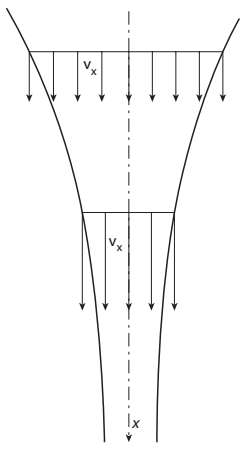
\includegraphics[width=0.4\textwidth]{Graphics/reo2.png}
    \caption[Flujo extensional uniaxial]{Flujo extensional uniaxial. Un material viscoso es estirado por una fuerza que actúa a lo largo de la dirección $x$. Adaptada de ().}
    \label{fig:reo2}
\end{figure}

\begin{equation}
\frac{\delta v_{y}}{\delta_{y}}=\frac{\delta v_{z}}{\delta_{z}}= -\frac{1}{2} \frac{\delta v_{x}}{\delta_{x}}
\end{equation}

Las componentes fuera de la diagonal principal son todas cero. Las velocidades en las direcciones $y$ y $z$ son idénticas por razones de simetría.
En casos de flujo mas complejos, ambas, las componentes de corte y extensionales pueden estar presentes. Por ejemplo en flujos convergentes, cuando un líquido fluye a través de una reducción. La fricción en la pared causa el corte, mientras que la reducción obliga al fluido a acelerarse para permitir que la misma cantidad de materia fluya a través de las secciones transversales. Esto induce una componente extensional.

\subsection{Dinámica}
Así como es necesario generalizar el gradiente de velocidad (ecuación 28) al tensor de tasa de deformación (ecuación 31), se debe adaptar la expresión del esfuerzo de corte para aplicarlo a casos mas generales de flujo. En el caso de flujo cortante simple, solo la componente del esfuerzo $\sigma_{xy}$ es considerada. La \autoref{fig:reo3} muestra un paralelepípedo alrededor de un punto en el seno del fluido, con sus lados paralelos a las planos coordenados. Los planos son identificados por su dirección normal al plano.

\begin{figure}\centering
    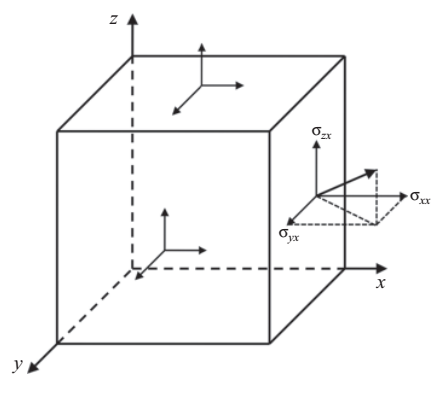
\includegraphics[width=0.7\textwidth]{Graphics/reo3.png}
    \caption[Componentes del esfuerzo de corte]{Componentes del esfuerzo de corte $\sigma$. Adaptada de ().}
    \label{fig:reo3}
\end{figure}

La fuerza $F_{i}$, sobre un plano arbitrario $A_{i}$ en el material, no está orientada de manera perpendicular ni paralela al plano. Dicha fuerza, o su correspondiente esfuerzo, en general se descompone en tres componentes. Para el plano $dA_{x}=d_{y}d_{z}$ perpendicular a la dirección $x$, las componentes dadas por el cociente $dF_{x}/dydz$ del esfuerzo son $\sigma_{xx},\sigma_{yx},\sigma_{zx}$ (\autoref{fig:reo3}). El primer subíndice se refiere a la dirección de la componente de esfuerzo mientras que el segundo se refiere a la normal al plano sobre la cual actúa el esfuerzo. Aplicando el mismo procedimiento al los esfuerzos en los demás planos coordenados, resulta en la matriz de componentes del esfuerzo $\sigma_{ij}$:

\begin{equation}
\sigma_{ij}=\left( \begin{matrix}
\sigma_{xx} & \sigma_{xy} & \sigma_{xz} \\
\sigma_{yx} & \sigma_{yy} & \sigma_{yz} \\
\sigma_{zx} & \sigma_{zx} & \sigma_{zz}
\end{matrix} \right)
\end{equation}

Se puede demostrar que los esfuerzos en cualquier plano de orientación arbitraria en un punto dado, pueden ser calculados a partir de las nueve componentes de esfuerzo sobre los planos coordenados. Los esfuerzos pueden ser expresados en varios sistemas de coordenadas, siguiendo ciertas reglas de transformación, como en el caso del gradiente de velociada y por lo tanto describen un tensor \textbf{$\sigma$}.

Así como con el tensor de tasa de deformación, se distinguen dos diferentes componentes del tensor de esfuerzo. Las componentes en la diagonal principal, $\sigma_{ii}$, están orientadas de manera normal al plano sobre el que actúan; estos son los \emph{esfuerzos normales}. Las componentes fuera de la diagonal principal, se encuentran orientados según el plano a considerar; estos son los \emph{esfuerzos de corte}. Para fluidos ordinarios se puede demostrar que la matriz de esfuerzos $\sigma_{ij}$ es simétrica con respecto a su diagonal principal (igual que el tensor de tasa de deformación).

\begin{equation}
\sigma_{ij}=\sigma_{ji}
\end{equation}

Aun cuando no existe flujo, existe una presión hidrostática en el fluido. Esto origina una presión idéntica (esfuerzo normal) en todas direcciones, mientras que los esfuerzos de corte son todos cero:

\begin{equation}
\sigma_{ij}= \left( \begin{matrix}
-P & 0 & 0 \\
0 & -P & 0 \\
0 & 0 & -P
\end{matrix} \right) = -P\left( \begin{matrix}
1&0&0 \\
0&1&0 \\
0&0&1
\end{matrix} \right)
\end{equation}

Por convención la presión es negativa y el tensor positivo. La matriz de la derecha representa el tensor unitario \textbf{I}, el cual se escribe en notación vectorial como:

\begin{equation}
\sigma=-PI
\end{equation}

La aplicación de un flujo cortante a un fluido newtoniano, resulta en esfuerzos de corte proporcionales al la velocidad de corte (gradiente de velocidad). En términos de tensores, la expresión para la ecuación constitutiva de Newton es:
\begin{equation}
\sigma = -PI+2\eta D
\end{equation}

en donde el \emph{esfuerzo extra} $\sigma +P\textbf{I}$ es el factor de relevancia para la reología dado que la presión no afecta el flujo de fluidos incompresibles. Las componentes normales del esfuerzo extra son siempre cero para fluidos newtonianos. La cantidad de energía (por unidad de volumen) requerida para el caso simple de flujo cortante en un fluido newtoniano es $\sigma : D=\eta \dot{\gamma^{2}}$ que se disipa como flujo de calor.

\subsection{Fluidos Newtonianos Generalizados}
Para la mayoria de las suspensiones, el esfuerzo de corte sn flujo cortante simple, no es proporcional a la velocidad de corte y por ello no satisfacen la ley de Newton; estos son \emph{no newtonianos}.

Como primer caso de fluido no newtoniano están aquellos para los cuales el esfuerzo de corte está determinado en todo momento por un valor instantáneo de velocidad de corte, pero que no es proporcional. Los fluidos de este tipo son \emph{fluidos newtonianos generalizados}. En este caso la viscosidad es definida como \emph{viscosidad aparente} puesto que es función de la velocidad de corte. La \autoref{fig:reo4} muestra las formas posibles de la función $\sigma(\dot{\gamma})$

\begin{figure}\centering
    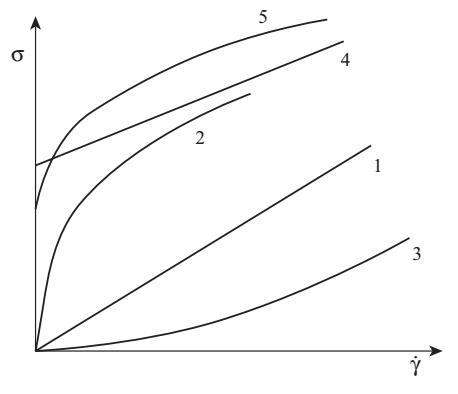
\includegraphics[width=0.7\textwidth]{Graphics/reo4.png}
    \caption[Curvas reológicas generales]{Curvas generales de esfuerzo de corte vs velocidad de corte. (1) Newtoniano; (2) Adelgazante; (4) Espesante; (5) Materiales con esfuerzo de cedencia Adaptada de ().}
    \label{fig:reo4}
\end{figure}

La curva (1) representa el caso newtoniano. En la curva (2) el esfuerzo de corte se incrementa por debajo de la proporciónal a la velocidad de corte, de manera que la viscosidad, (el cociente entre ambos) decrece con el incremento en la velocidad de corte. Este comportamiento describe un adelgazamiento al corte. El caso opuesto es la curva (3), donde la viscosidad se incrementa con el aumento de la velocidad de corte, \emph{Engrosamiento al corte}. Algunas sustancias pueden presentar ambos comportamientos dependiendo de la región de velocidad de corte en la que se encuentran.

Las curvas (2) y (3) representan relaciones no lineales entre el esfuerzo de corte y la velocidad de corte, pero al ser graficados de manera logarítmica se ajustan a una línea recta, lo que significa que esta relación se puede describir con una ley de potencias:

\begin{equation}
\sigma = k\dot{\gamma^{n}}
\end{equation}

donde $n$ el índice de ley de potencias, es la pendiente de la recta en una gráfica logarítmica.

De manera que la ecuación constitutiva de Newton para fluidos de este tipo es conocida como ley de potencias, donde para $n<<1$ se describe un adelgazamiento y $n>1$ describe un engrosamiento. La viscosidad en un fluido ley de potencias cambia de manera proporcional a $\dot{\gamma^{n-1}}$. Para $n<1$, la viscosidad se incrementa indefinidamente ($\eta_{\infty}$) a medida que la velocidad de corte tiende a cero, y por el contrario la característica asintótica de la curva hace que para velocidades de corte altas la viscosidad tiende a cero ($\eta_{0}$), de manera que estas curvas de viscosidad se describen mediante el modelo de viscosidad de \emph{Cross} (REF 27):

\begin{equation}
\eta-\eta_{\infty}=\frac{\eta_{0}-\eta_{\infty}}{1+(k^{'}\dot{\gamma})^{m}}
\end{equation}

Para fluidos cuyo comportamiento se puede describir mediante las ecuaciones (39) y (40) el esfuerzo de corte disminuye hacia cero a medida que la velocidad de corte tiende a cero, pero siempre debe existir una velocidad de corte diferente de cero, para producir un esfuerzo de corte diferente de cero. De manera que el fluido no puede existir en equilibrio bajo un esfuerzo de corte diferente de cero.

Algunos materiales exhiben un valor de esfuerzo de corte finito y diferente de cero, cuando la velocidad de corte es disminuida sistemáticamente, como en el caso de las curvas (4) y (5) en la \autoref{fig:reo4}. Mientras que para valores de velocidad de corte altos aún presentan un comportamiento newtoniano. La curva (4) describe un \emph{cuerpo de Bingham}:

\begin{equation}
\sigma = \sigma^{B}_{y} + \eta_{pl}\dot{\gamma}
\end{equation}

donde las características de del material son el esfuerzo de cedencia de Bingham $\sigma^{B}_{y}$ y la viscosidad plástica $\eta_{pl}$. Cuando el límite superior de velocidad de corte describe una ley de potencias, mas que un comportamiento newtoniano, se puede utilizar el modelo de \emph{Herschel-Bulkley}:

\begin{equation}\centering
\sigma= \sigma^{H}_{y}+k\dot{\gamma^{n}}
\end{equation}

%Adicionalmente existe un tercer modelo usado con frecuencia para describir a las supensiones con esfuerzo de cedencia:
%\begin{equation}
%\sigma^{n}=\sigma^{n}_{y}+k\dot{\gamma^{n}}
%\end{equation}
%cuando $n=1/2$ esta se convierte en la ecuación de \emph{Casson}, que es un modelo utilizado para describir el flujo sanguineo.

Adicional al esfuerzo de cedencia algunas suspensiones presentan otra complicación, la viscosidad no es solo función del la velocidad de corte instantánea, si no que la agitación o el corte ocasionan una disminución gradual en la viscosidad, la cual se recupera cuando el material esta en reposo. Una viscosidad dependiente del tiempo pero reversible define el concepto de \emph{tixotropía}. 

\subsection{Viscoelasticidad}

Los materiales \emph{viscoelásticos} combinan las propiedades elásticas de los sólidos con las de los fluidos viscosos. Los esfuerzos en un cuerpo elástico dependen de que tan grande es la desviación en la forma actual del cuerpo, de su forma original no deformada ni sometida a esfuerzo alguno, independientemente de la escala de tiempo de la deformación. Siempre que un esfuerzo haya sido aplicado, incluso por un largo tiempo, un material elástico siempre regresa a su estado no deformado cuando los esfuerzos son retirados. De manera ideal un material elástico tiene una perfecta "memoria" para regresar a su configuración no deformada. Un líquido, por otro lado, no posee esta memoria, de modo que aún cuando el esfuerzo de corte es retirado el fluido permanece en la última posición alcanzada.

Al aplicar de manera repentina una deformación de corte y mantenerla constante, en un sólido elástico el esfuerzo resultante permanecerá constante de manera indefinida. En un líquido el esfuerzo será muy alto cuando la deformación es aplicada de manera rápida, pues la velocidad de corte sera muy alta, pero una vez que termina la rápida deformación, no habrá flujo y el esfuerzo caerá inmediatamente a cero. Por otra parte en un material viscoelástico, el esfuerzo al corte disminuirá gradualmente en el tiempo, este fenómeno es conocido como \emph{relajación del esfuerzo}. Si el material viscoelástico es un sólido el esfuerzo se relajará parcialmente hasta un valor finito, mientras que si se trata de un líquido el esfuerzo se relaja hasta el valor de cero. 

Si retomamos el caso de flujo cortante de la figura \autoref{fig:reo1}, pero ahora en lugar de de moverse con una velocidad constante,la placa superior ejerce un movimiento sinusoidal $X_{p}(t) = X_{p,0}~seno(\omega t)$, donde $X_{p,0}$ pico máximo del desplazamiento. Esto genera una deformación dependiente del tiempo $\gamma(t)$ (linea continua en la 
\autoref{fig:reo5})

\begin{figure}
    \centering
    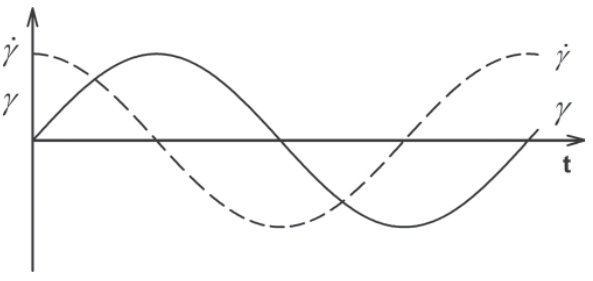
\includegraphics[width=0.8\textwidth]{Graphics/Reo5.png}
    \caption[Deformación en flujo oscilatorio]{Deformación, dependiente del tiempo, generada por una placa que ejerce un movimiento sinusoidal. Adaptada de ().}
    \label{fig:reo5}
\end{figure}
%
%
%
%
%
%                           E            S             P           A           C          I         O
%
%
%
%
\subsection{Geles}
%Ejemplo del slim     alcohol polivinilico + tetraborato de sodio interacciones moleculares quimica supramolecular fuerzas de londo, ion dipolo, 
%PLATEAU:a state of little or no change following a period of activity or progress.
\begin{description}
\item[Definición] En términos generales un gel puede ser definido como un estado intermedio de la materia entre el comportamiento reológico de sólido y el de un líquido. Consiste de una fase dispersa (polímero o coloide) y un medio de dispersión (agua u otro solvente), y puede ser muy semejante a un líquido o a un sólido. Su característica líquida se debe a que el mayor constituyente es el solvente. Su comportamiento de sólido proviene de la red formada por retículos que impide que el gel fluya y se caracteriza por tener un módulo elástico finito (\cite{Nishinari2009}).
%\item[Retículo] Según la \emph{IUPAC} \cite{IUPAC2} se trata de una región pequeña en un macromolécula en la cual al menos se forman cuatro cadenas formadas por reacciones o grupos de moléculas, o por interacciones entre moléculas existentes. Una región pequeña puede tratarse de un átomo, un grupo de átomos o un número de ramificaciones conectadas por enlaces, grupos de átomos o cadenas oligoméricas. En la mayoría de los casos un retículo es una estructura covalente sin embargo se utiliza también para describir interacciones químicas más débiles e incluso interacciones físicas.
\end{description}


Un gel puede ser definido de manera reológica o de manera estructural, En términos de su reología, un gel es un sistema que no fluye y que puede ser caracterizado por la presencia en su reograma de una zona meseta del módulo de almacenamiento y una valor de $tan(\delta) < 0.1$ en un rango de frecuencia angular de $10^{-3}~a~10^{2}~~rad/s$. Estructuralmente un gel es definido por la conectividad del sistema. Un gel en un sistema que consiste de moléculas, partículas, cadenas, etc. que está parcialmente conectadas una con otra por retículos a escala macroscópica.

\subsubsection{Clasificación reológica}
Dado que este trabajo hace hincapié en la definición reológica de gel, es importante mencionar que algunos autores han clasificado el comportamiento reológico de los geles en cuatro grandes grupos de acuerdo con su espectro mecánico, la dependencia del modulo de almacenamiento y el modulo de pérdida (\emph{G' y G''} respectivamente) con la frecuencia, en un rango aceptablemente accesible a la tecnología comercial de entre $10^{-3}~a~ 10^{2}~~rad/s$ (\cite{Clark}).

\begin{itemize}
    \item 1. Gel Fuerte (gel elástico o verdadero). \emph{G'} es mucho más grande que \emph{G''} y ambos módulos son independientes de la frecuencia.
    \item 2. Gel débil (líquido estructurado). \emph{G'} ligeramente más grande que \emph{G''} y ambos módulos son ligeramente dependientes de la frecuencia.
    \item 3. Polímero entrecruzado. \emph{G'} es más pequeño que \emph{G''} para frecuencias mas bajas, pero ambos módulos se incrementan con el incremento de frecuencia y muestran un cruce luego del cual \emph{G'} se vuelve más grande que \emph{G''} para frecuencias mas altas.
    \item 4. Polímero no entrecruzado. \emph{G'} es mucho más pequeño que \emph{G''} para cualquier frecuencia y ambos módulos son fuertemente dependientes de la frecuencia.
\end{itemize}

El reograma típico para un líquido estructurado se muestra en la \autoref{fig:estructurado}.

\begin{figure}\centering
    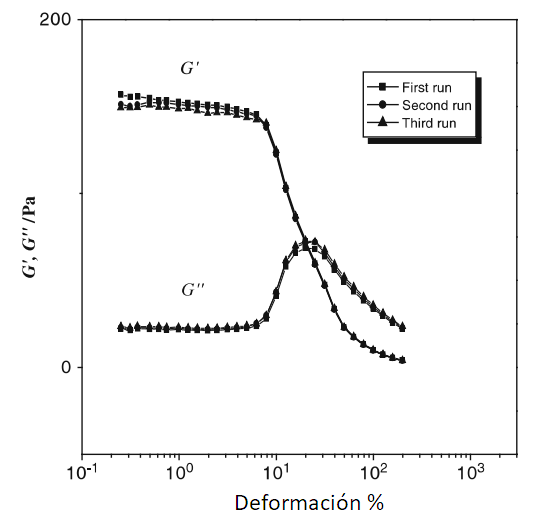
\includegraphics[width=0.9\textwidth]{Graphics/weak_gel}
    \caption[Reograma de un gel débil.]{Dependencia de los módulos de almacenamiento \emph{G'} y pérdida \emph{G''} con la deformación. Reograma típico de un gel débil o fluido estructurado. Obtenido mediante un barrido de deformación con una frecuencia angular de 1 rad/s. Ejemplo de una solución acuosa de SPG-sorbitol.Adaptada de (\cite{Nishinari2009})}
    \label{fig:estructurado}
\end{figure}


%\chapter{Reología}
\label{chp:reologia}

\section{Introducción}

\section{Generalidades}
\section{Reología de dispersiones}
\section{Reología de surfactantes en solución}
\subsection{Reología de Geles}
%\input{Chapters/Descripción del campo}     % Así agregamos un capitulo nuevo
\chapter{Metodología}
\label{chp:metodologia}

\section{Introducción}

En el presente capítulo se presenta, de manera secuencial, la exploración general llevada a cabo en laboratorio para buscar la evidencia de la formación del organogel en el sistema multifásico aceite-salmuera-surfactante (\textbf{A-S-S}). El trabajo realizado incluye la preparación de varias series de pruebas de botella, mediciones reométricas, y toma de imágenes de microscopía La descripción técnica de los equipos de laboratorio utilizados se incluye el anexo A.

\section{Fluidos Utilizados}
Para llevar a cabo la reproducción del sistema multifásico A-S-S, se utilizó aceite hidrocarburo muestreado en cabeza de pozo, proveniente del pozo Teotleco-$42$ e identificado como \emph{Teotleco E$2015$-$1465$} cuyas propiedades se muestran en la \autoref{tab:aceite}. El muestreo en cabeza de pozo, proporciona una muestra de fluido previo a la adición de aditivos para su estabilización. La salmuera identificada como \emph{Salmuera E$2015$-$1465$} y cuyas propiedades se muestran en la \autoref{tab:salmuera} proviene de la misma muestra de cabeza, esta salmuera se filtra antes de ser usada, se prefiere este fluido por encima de una salmuera sintética dado que la alta salinidad, representa una dificultad para estabilizar una salmuera de composición controlada.

Para el surfactante se eligieron dos lotes distintos del mismo producto llamados \emph{Amesus $3100$} y \emph{Amesus $3200$}, la diferencia entre ambos lotes radica en...

\begin{table}
\caption[Aceite E$2015$-$1465$] {Propiedades de la muestra de aceite E$2015$-$1465$.}
\centering
\begin{tabulary}{1.1\textwidth}{L |R}
    \toprule
    Gravedad API & $39.79$ \\
    Densidad [$g/cm^{3}$] & $0.82442$ \\
    Viscosidad [cp] & $29$  \\
    \midrule
    \bottomrule
\end{tabulary}
\label{tab:aceite}
\end{table}

\begin{table}
    \caption[Salmuera E$2015$-$1465$] {Propiedades del muestra de salmuera E$2015$-$1465$.}
    \centering
    \begin{tabulary}{1.1\textwidth}{L |R}
        \toprule
        Salinidad [ppm] & $160000$ \\
        Densidad [$g/cm^{3}$] & $1.1614$ \\
        Viscosidad [cp] & $13$  \\
        \midrule
        \bottomrule
    \end{tabulary}
    \label{tab:salmuera}
\end{table}

\section{Pruebas de Botella}
Se prepararon $7$ muestras de $100$ ml cada una de salmuera con tensoactivo y aceite, en una relación $50$-$50$ \textit{v/v}, con diferente concentración del \emph{Amesus$3100$}, los volúmenes para la preparación se muestran en la \autoref{tab:serie1}. Posterior a la mezcla las muestras fueron agitadas mecánicamente durante un tiempo de $3$ minutos y preservadas en un horno a $70$\celsius.

 \begin{table} 
    \caption[Pruebas de botella]{Serie $1$ Pruebas de botella del sistema A-S-S a diferentes concentraciones de surfactante.}
    \centering
    \begin{tabulary}{1.1\textwidth}{L |R|R|R|R|R|R|R}
        \toprule
        Botella & \textbf{1} & \textbf{2} & \textbf{3} & \textbf{4} & \textbf{5} & \textbf{6} & \textbf{7} \\
        \midrule
        Concentración [\%] & $0.5$  & $1$ & $3$  & $5$ & $10$ & $13$ & $15$ \\
        Amesus ~~~~~~~~~~[ml] & $0.3$  & $0.5$ & $1.5$ & $2.5$ & $5.0$ & $6.5$ & $7.5$ \\
        Salmuera ~~~~~~~~[ml] & $49.8$ & $49.5$ & $48.5$ & $47.5$ & $45$ & $43.5$ & $42.5$ \\
        Aceite ~~~~~~~~~~~~~[ml] & $50$ & $50$ & $50$ & $50$ & $50$ & $50$ & $50$ \\
        \midrule
        \bottomrule
    \end{tabulary}
    \label{tab:serie1}
\end{table}

Se registró en fotografías el drenado de las fases salmuera y emulsión organogel en el sistema formado durante $10$ días. La intención de este experimento es evidenciar mediante análisis de imágenes el cambio en la composición de la fase emulsionada y salmuera.


\section{Reometría}
Con  el  propósito  de  evaluar  el  efecto  de  la  concentración  del producto Amesus $3100$, la presión y la temperatura sobre las propiedades reológicas del sistema se realizaron los siguientes experimentos. Se preparó una nueva serie de muestras que a $3$ concentraciones de producto distintas, las cuales se presentan en la \autoref{tab:serie2}. De cada muestra se analizó su comportamiento reológico tanto para la parte emulsionada como para la salmuera no emulsionada. Para la caracterización reológica del sistema se utilizó un reómetro \emph{Physica MCR} de la marca \emph{Anton Paar}, con una geometría de medición de cilindros concéntricos, y una cámara de presión con calentamiento eléctrico.

 \begin{table} 
    \caption[Efecto de la concentración]{Serie $2$ Pruebas de botella del sistema A-S-S a diferentes concentraciones de surfactante.}
    \centering
    \begin{tabulary}{1.1\textwidth}{L |R|R|R|}
        \toprule
        Botella & \textbf{1} & \textbf{2} & \textbf{3} \\
        \midrule
        Concentración [\%] & $5$  & $10$ & $15$ \\
        Amesus ~~~~~~~~~~[ml] & $1.25$  & $2.5$ & $3.75$  \\
        Salmuera ~~~~~~~~[ml] & $23.75$ & $22.5$ & $21.25$ \\
        Aceite ~~~~~~~~~~~~~[ml] & $25$ & $25$ & $25$  \\
        \midrule
        \bottomrule
    \end{tabulary}
    \label{tab:serie2}
\end{table}

%******************************************************************************
%*
%*    DESCRIPCION DEL REOMETRO Y LA GEOMETRIAS Y LA CÁMARA DE PRESIÓN
%*
%******************************************************************************
Se compararon los reogramas de cada muestra al momento de la preparación y $24$ horas después de la preparación. Las siguientes condiciones de medición para cada experimento fueron:

\begin{description}
    \item [Prueba A] Viscosidad vs velocidad de corte a $23$ \celsius~ y $14.7$ psi, con una rampa de velocidad de corte $2$ a $100 ~ s^{-1}$.
    \item [Prueba B] Viscosidad vs velocidad de corte a $23$ \celsius~ y $1500$ psi, con una rampa de velocidad de corte $2$ a $100 ~ s^{-1}$.
    \item [Prueba C] Viscosidad vs velocidad de corte a $160$ \celsius~ y $1500$ psi, con una rampa de velocidad de corte $2$ a $100 ~ s^{-1}$.
    \item [Prueba D] Viscosidad vs temperatura a presión constante de $1500$ psi y velocidad de corte de $100 ~ s^{-1}$, con una rampa de temperatura de $23$ a $160$ \celsius.
\end{description}

Adicionalmente se llevo a cabo la \textbf{prueba D} para el aceite libre observado durante las pruebas de botella. Para este experimento se contaba con una muestra adicional con una concentración de Amesus $3100$ del $3$\% con una preparación similar a las anteriores y se incluyó como muestra el aceite original sin producto.

Posteriormente se analizó el efecto de la salinidad de la salmuera sobre el comportamiento reológico en presencia del surfactante, preparándose una salmuera sintética en diferentes concentraciones de cloruro de sodio resumidas en la \autoref{tab:serie3}. En todos los casos la concentración de Amesus $3100$ fue del $10\%$ y el volumen final de las muestras fue de $50$ ml. Las botellas fueron agitadas durante $3$ minutos para posteriormente llevar a cabo las siguientes pruebas:

 \begin{table} 
    \caption[Efecto de la salinidad]{Serie $3$ Pruebas de botella del sistema A-S-S a diferentes concentraciones de NaCl.}
    \centering
    \begin{tabulary}{1.1\textwidth}{L |R|R|R|R|R|}
        \toprule
        Botella & \textbf{1} & \textbf{2} & \textbf{3} & \textbf{4} & \textbf{5}  \\
        \midrule
        Concentración [ppm] & $20$  & $50$ & $70$  & $100$ & $120$ \\
        NaCl ~~~~~~~~~~~~~~[mg] & $1000$  & $2500$ & $3500$ & $5000$ & $6000$ \\
        Amesus ~~~~~~~~~~[ml] & $5$ & $5$ & $5$ & $5$ & $5$ \\
        Agua ~~~~~~~~~~~~~~[ml] & $45$ & $45$ & $45$ & $45$ & $45$ \\
        
        \midrule
        \bottomrule
    \end{tabulary}
    \label{tab:serie3}
\end{table}


\begin{description}
    \item [Prueba A] Viscosidad vs velocidad de corte a $23$ \celsius~ y $14.7$ psi, con una rampa de velocidad de corte $2 a 100~ s^{-1}$.
    \item [Prueba B] Viscosidad vs velocidad de corte a $23$ \celsius~ y $1500$ psi, con una rampa de velocidad de corte $2$ a $100~ s^{-1}$.
    \item [Prueba D] Viscosidad vs temperatura a presión constante de $1500$ psi y velocidad de corte de $100~s^{-1}$, con una rampa de temperatura de $23$ a $70$ \celsius.
    \item [Prueba F] Viscosidad vs velocidad de corte a $70$ \celsius~ y $1500$ psi, con una rampa de velocidad de corte $2$ a $100~ s^{-1}$.
\end{description}


\subsection*{Punto de cedencia}

Se propone evaluar el reograma en con condiciones de esfuerzo oscilatorio para demostrar que las fases emulsionadas que se generan durante las pruebas de botella poseen propiedades visco elásticas. Para evaluar las implicaciones de este fenómeno se preparan una nueva serie de muestras A-S-S, las concentraciones y volúmenes de cada muestra se presentan en la \autoref{tab:serie4}.

 \begin{table}[H]
    \caption[Pruebas de botella]{Serie $4$ Pruebas de botella del sistema A-S-S a diferentes concentraciones de surfactante.}
    \centering \footnotesize
    \begin{tabulary}{1.1\textwidth}{L |R|R|R|R|R|R|R}
        \toprule
        Botella & \textbf{1} & \textbf{2} & \textbf{3} & \textbf{4}  \\
        \midrule
        Concentración [\%] & $5$  & $10$ & $13$  & $15$  \\
        Amesus ~~~~~~~~~~[ml] & $1.25$  & $2.5$ & $3.25$ & $3.75$  \\
        Salmuera ~~~~~~~~[ml] & $23.75$ & $22.5$ & $21.75$ & $21.25$  \\
        Aceite ~~~~~~~~~~~~~[ml] & $25$ & $25$ & $25$ & $25$  \\
        \midrule
        \bottomrule
    \end{tabulary}
    \label{tab:serie4}
\end{table}

Se realizaron mediciones del módulo complejo y el módulo de almacenamiento, en una prueba de flujo oscilatorio con un barrido de deformación de $0.1$\% a $100$\% y una frecuencia angular de $0.5$ rad/s.

\begin{description}
    \item [Prueba G1] Módulos complejo y de almacenamiento vs velocidad de corte en flujo oscilatorio a $23$ \celsius~ y $14.7$ psi, con una rampa de deformación de $0.1 a 100~ \%$, amplitud de $XX~rad$ y frecuencia angular de $0.5~rad$.
    \item [Prueba G2] Módulos complejo y de almacenamiento vs velocidad de corte en flujo oscilatorio a $70$ \celsius~ y $14.7$ psi, con una rampa de deformación de $0.1 a 100~ \%$, amplitud de $XX~rad$ y frecuencia angular de $0.5~rad$.
\end{description}


\subsection*{Tiempo de re-estruturación}
Adicionalmente se realizan mediciones de viscosidad vs velocidad de corte, intercaladas con un periodo de reposo, que permita capturar cualitativamente la reestructuración del sistema después de ser sometida al corte.

\section{Análisis de imágenes de microscopia}
Se propone realizar la microscopia para cada una de las fases formadas en las pruebas de botella, estas son llevadas a alta presión en un reactor Parr (\autoref{fig:tubos} \textbf{a}) para monitorear la morfología del sistema con el tiempo, a fin de describir al menos de manera cualitativa los procesos que tienen lugar y su posible relación con las propiedades reológicas. Las muestras analizadas y su concentración se resumen en la \autoref{tab:serie5}. Esta serie se preparó por duplicado cambiando únicamente el producto surfactante de \emph{Amesus $3100$} en la primera y \emph{Amesus $3200$} para la otra. Se preparan a temperatura ambiente y son agitadas mecánicamente por $3$ minutos como las anteriores (\autoref{fig:tubos} \textbf{b}).

\begin{figure}
    \centering 
    \subfloat[]{\rotatebox{90}{
        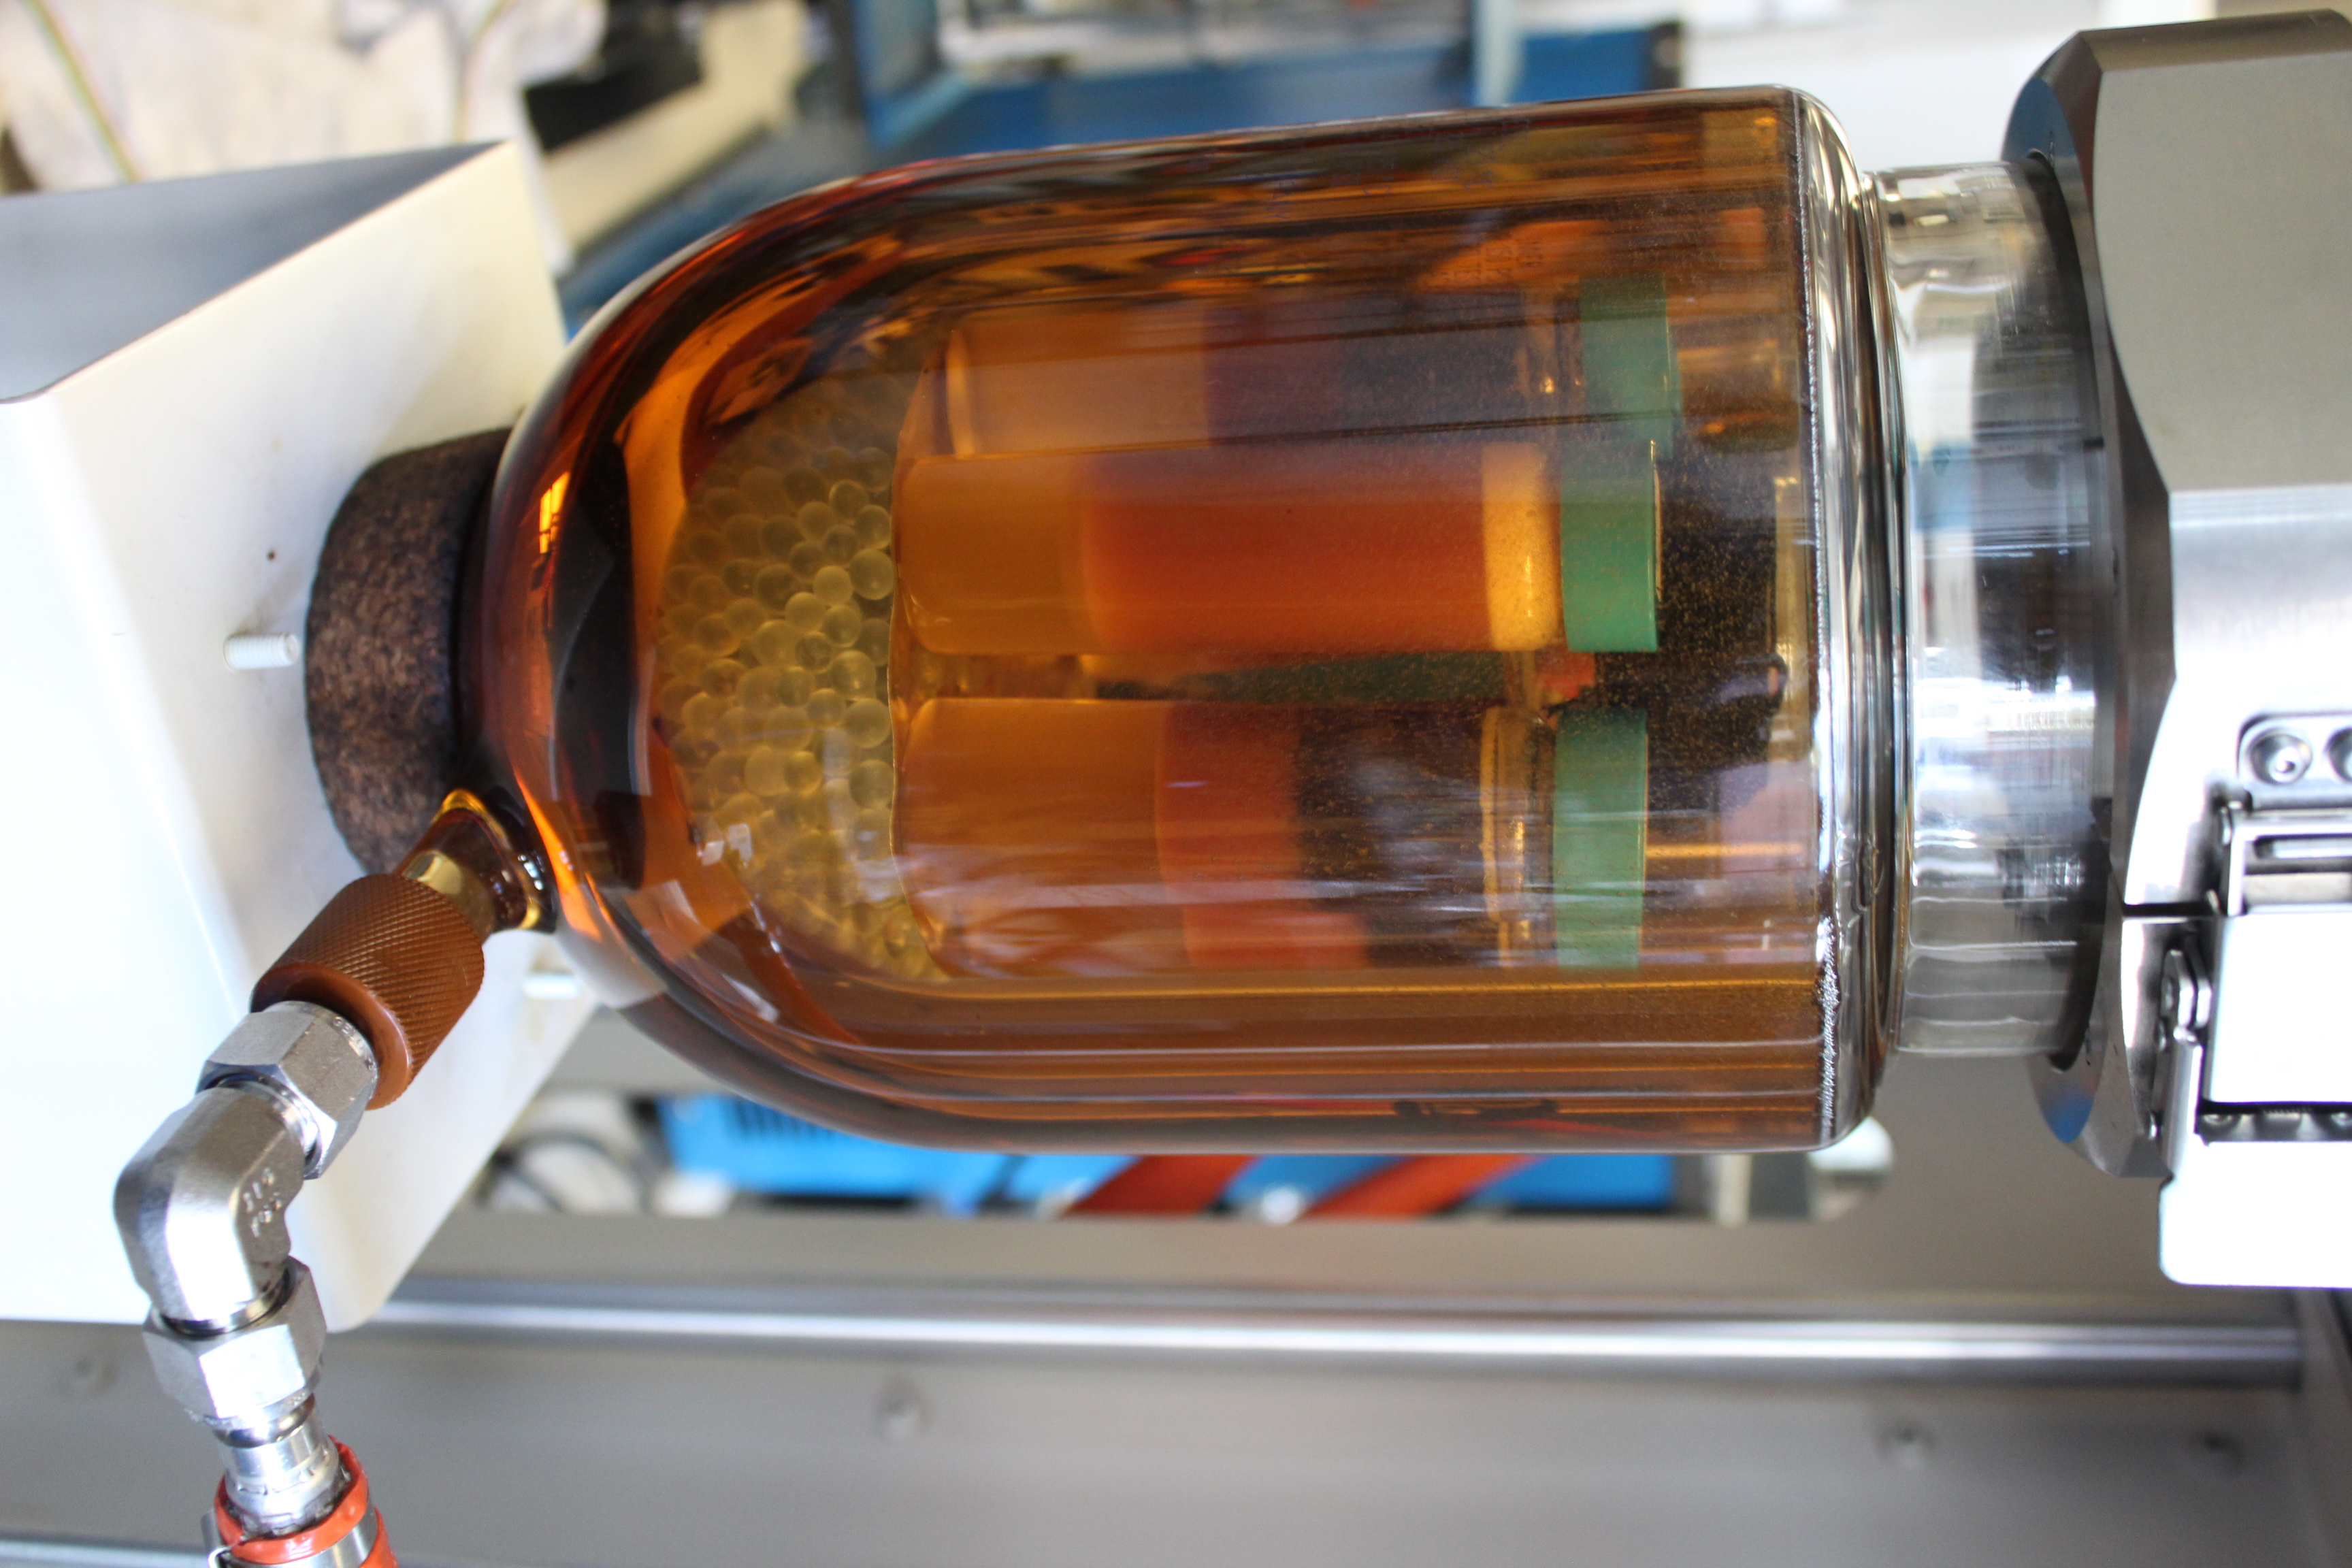
\includegraphics[width=0.5\textwidth]{Graphics/reactubos.JPG} } }
    \subfloat[]{
        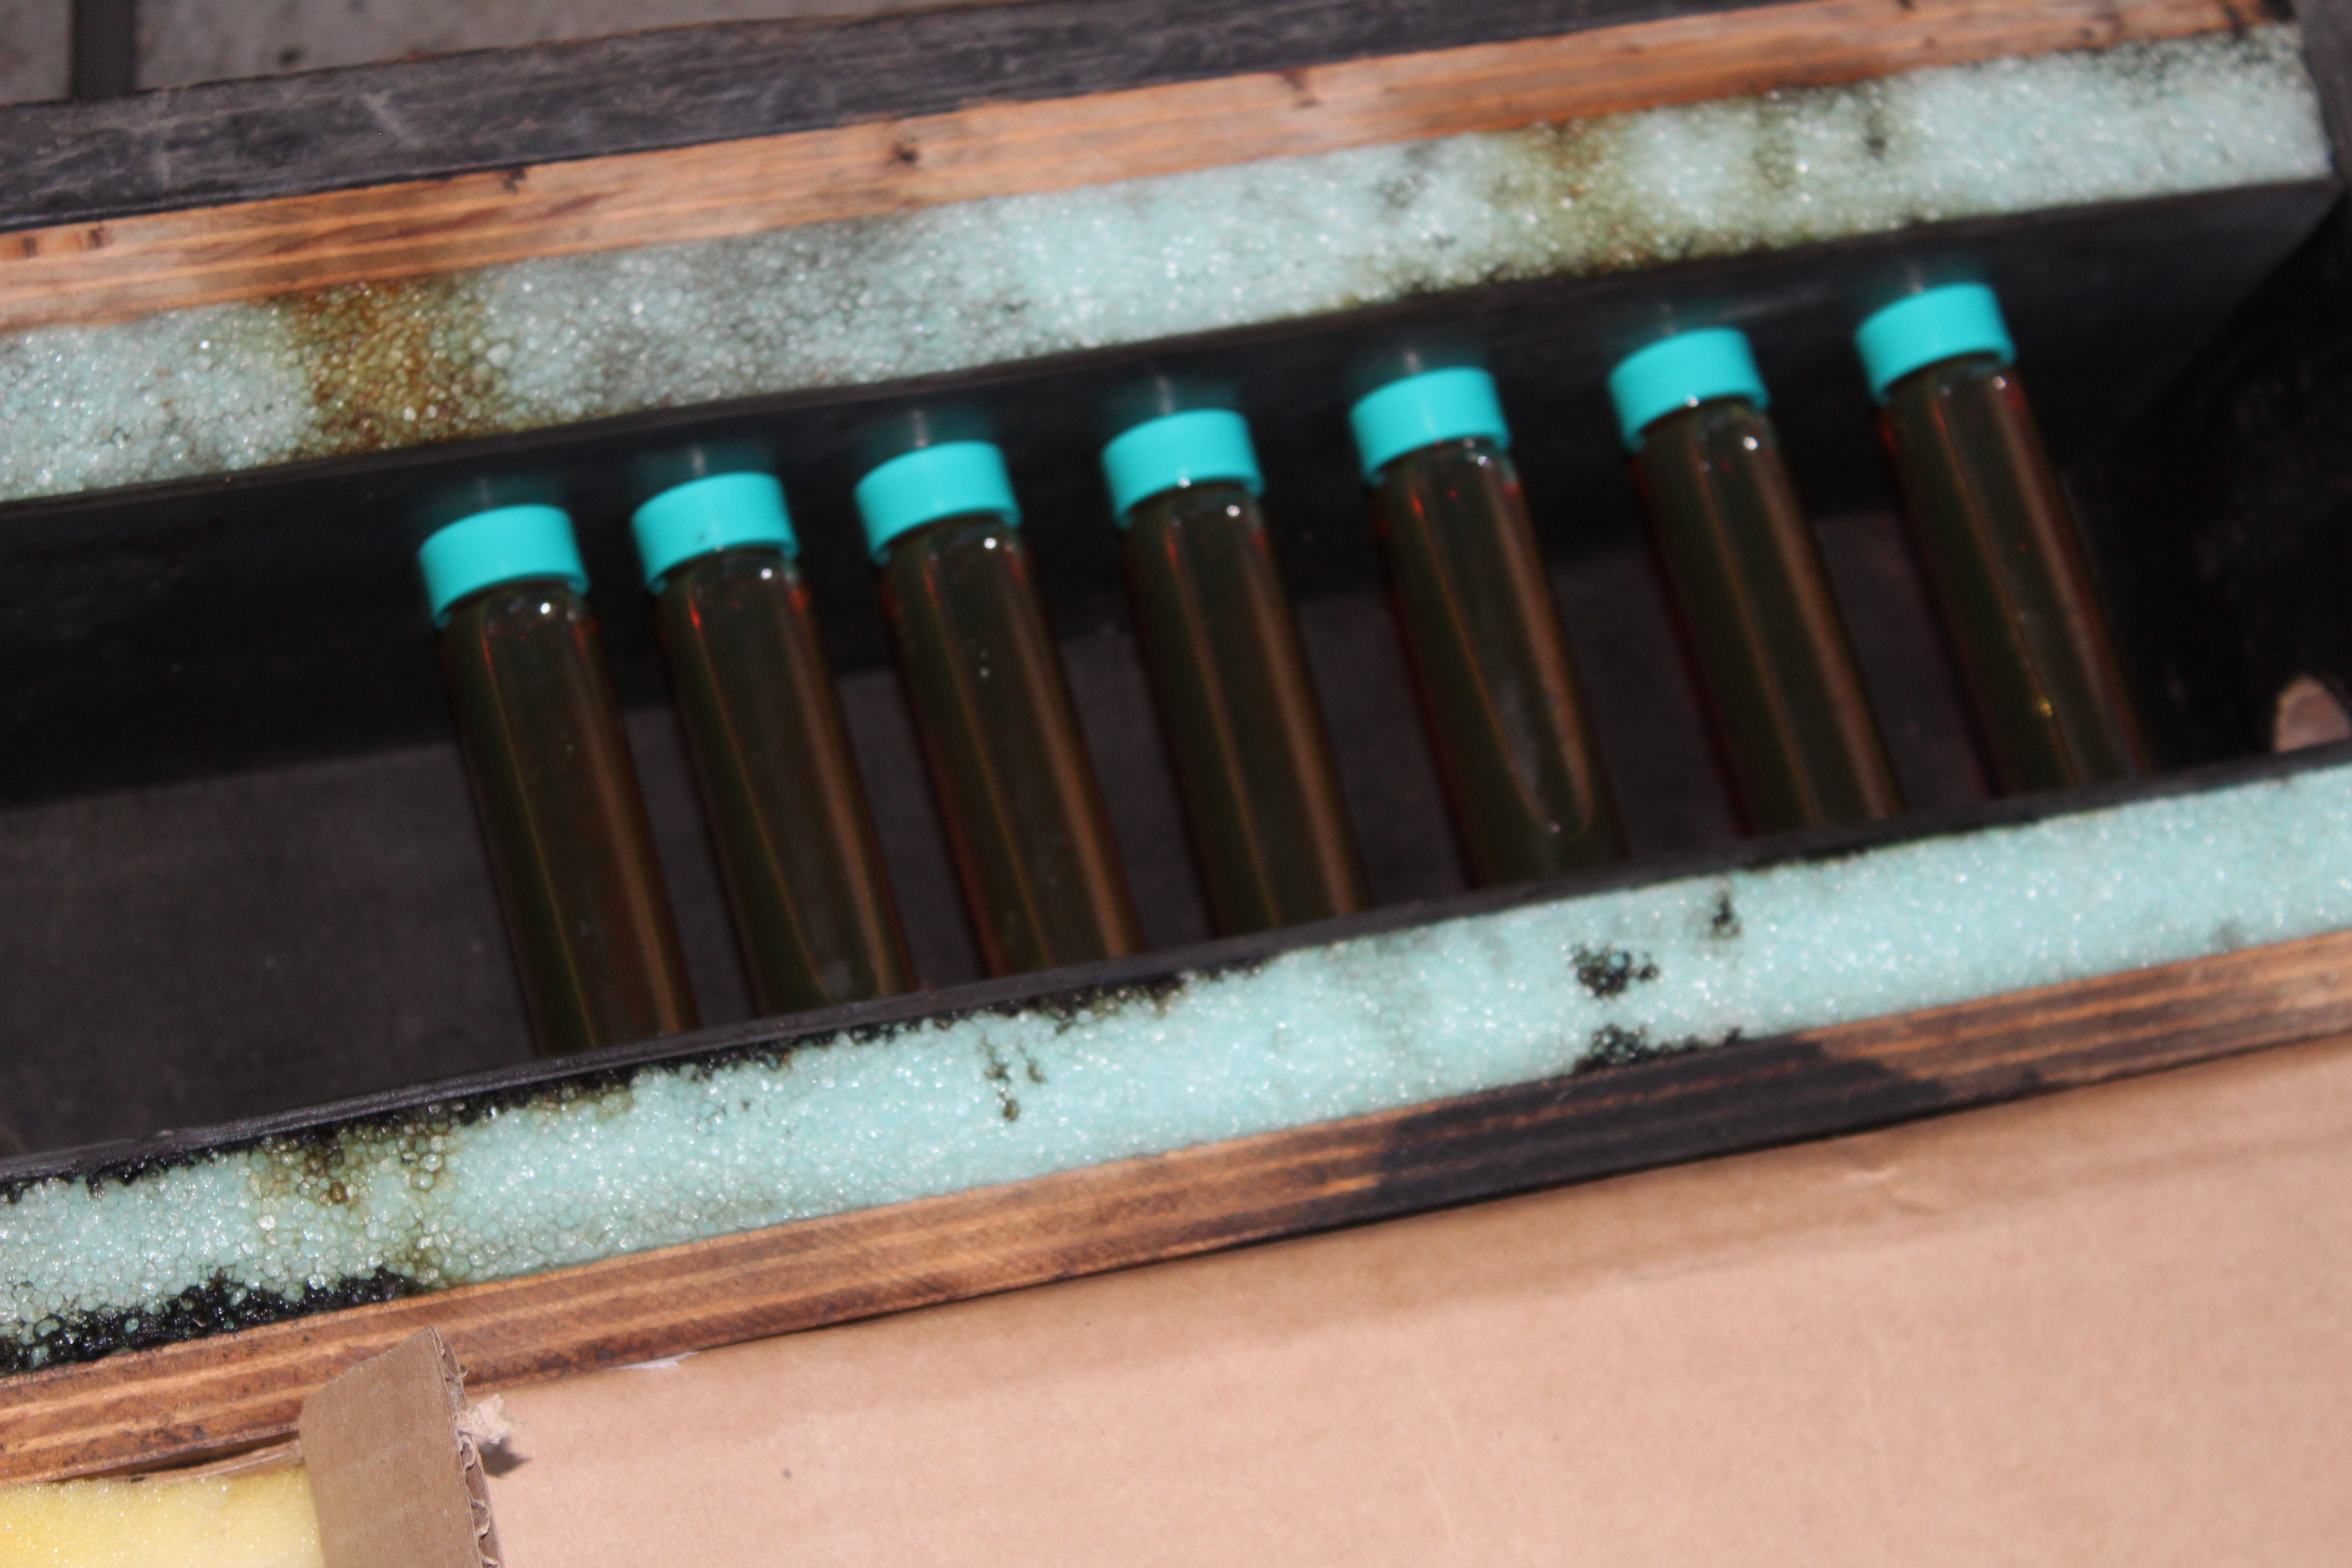
\includegraphics[width=0.5\textwidth]{Graphics/agitubos.JPG} }
    \caption[Muestras en tubos]{\textbf{(a)} Arreglo experimental en reactor Paar. \textbf{(b)} Agitador mecánico. }
    \label{fig:tubos}
\end{figure}

 \begin{table}[H]
    \caption[Pruebas de botella]{Serie $5$ Pruebas de botella del sistema A-S-S a diferentes concentraciones de surfactante.}
    \centering \footnotesize
    \begin{tabulary}{1.1\textwidth}{L |R|R|R|R|R|R|R}
        \toprule
        Botella & \textbf{1} & \textbf{2} & \textbf{3} & \textbf{4} & \textbf{5} & \textbf{6} & \textbf{7}  \\
        \midrule
        Concentración [\%] & $0.5$  & $1$ & $3$  & $5$ &$10$ & $13$ & $15$ \\
        Amesus ~~~~~~~~~~[ml] & $0.075$  & $0.15$ & $0.45$ & $0.75$ & $1.5$ & $1.95$ & $2.25$\\
        Salmuera ~~~~~~~~[ml] & $14.925$ & $14.85$ & $14.55$ & $14.25$ & $13.5$ & $13.05$ & $12.75$  \\
        Aceite ~~~~~~~~~~~~~[ml] & $15$ & $15$ & $15$ & $15$ & $15$ & $15$ & $15$  \\
        \midrule
        \bottomrule
    \end{tabulary}
    \label{tab:serie5}
\end{table}

Para cada serie se registra el nivel de las fases formadas en fotografías por XX días y mediante un algoritmo de conteo de pixeles, se registran los niveles de cada foto. Posteriormente se toma una muestra de cada fase formada y es montada en un microscopio.

\section{Tensión Interfacial}
Se llevaran a cabo mediciones de tensión interfacial en el sistema salmuera-aceite, aceite-aire, salmuera-organogel, y su comportamiento en con la concentración de surfactante. Esta información pretende ayudar a entender los procesos que ocurren dentro del sistema y permitirá complementar la descripción reológica. Para ello se utilizó un tensiómetro gota pendiente \emph{Krüss DSA} (\autoref{fig:Kruss}).
\begin{figure}\centering
    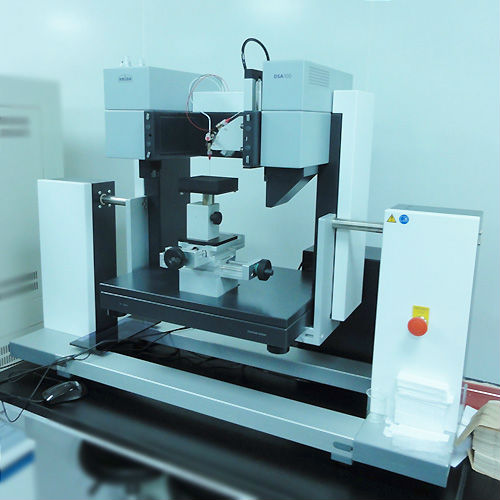
\includegraphics[width=0.6\textwidth]{Graphics/Kruss.jpg}
    \caption[Tensiómetro de gota]{Tensiómetro de gota pendiente Krüss DSA del Instituto Mexicano del Petróleo.}
    \label{fig:Kruss}
\end{figure}

Se prepararon $50$ ml de una solución madre de salmuera con $20000$ ppm de Amesus $3200$ en un matraz aforado, a partir de la cual se hicieron diluciones, el detalle de los volúmenes y concentraciones logradas se presenta en la \autoref{tab:diluciones}.

\begin{table}
    \caption[Diluciones]{Serie de diluciones a diferentes concentraciones de surfactante y salmuera.}
    \centering
    \begin{tabulary}{\textwidth}{|L|L|L|L|}
    \toprule
    Concentracion & \multicolumn{2}{c|}{Amesus 3200 } & Densidad \\
    \midrule
    ~ [ppm] & mg / $50$ ml & mg/ml & $\rho ~ [g/cm^{3}]$ \\
    \midrule
    20000 & 1000 & 20 & 1.15053 \\
    10000 & 500 & 10 & 1.15389 \\
    5000 & 250 & 5 & 1.15679 \\
    2500 & 125 & 2.5 & 1.15765\\
    1250 & 62.5 & 1.25 & 1.15936\\
    625 & 31.25 & 0.625 & 1.16064 \\
    325 & 16.25 & 0.325 & 1.16112 \\
    162.5 & 8.125 & 0.1625 & 1.16124 \\
    143 & 7.15 & 0.143 & 1.16133 \\
    65 & 3.25 & 0.065 & 1.161335 \\
    0 &0&0& 1.16140 \\
    \midrule
    \bottomrule
    \end{tabulary}
    \label{tab:diluciones}
\end{table}

Para la correcta determinación del diámetro de aguja utilizado, se utilizó un micrómetro con resolución de $0.01~mm$ y se calibro el sistema con agua tri-destilada y des-ionizada, de manera que a condiciones atmosféricas obtuviéramos el valor de tensión interfacial del agua, resultando en un diámetro de $0.9$ mm. En primer lugar se realizaron mediciones de tensión interfacial para el sistema Aire-Salmuera-Surfactante en todo el rango de concentraciones mostrado en la tabla anterior, utilizando como referencia el valor de densidad del aire al $16$ de mayo de $2017$ para la CDMX según el sistema meteorológico nacional que es de $1.1913264 kg/cm^{3}$.

Posteriormente se realizó la medición de tensión interfacial del sistema Aceite-Salmuera-Surfactante y finalmente para el sistema Salmuera-Organogel. Cada medición consiste de una fotografía de la gota, y su análisis mediante el algoritmo del equipo, similar al descrito en el \autoref{chp:antecedentes} de este trabajo.

\chapter{Resultados}
\label{chp:resultados}

\section{Introducción}

En el presente capítulo se presenta, de manera secuencial, los resultados de la exploración general llevada a cabo en laboratorio para buscar la evidencia de la formación del organogel en el sistema multifásico aceite-salmuera-surfactante (\textbf{A-S-S}). El trabajo realizado incluye la preparación de varias series de pruebas de botella, mediciones reométricas, y toma de imágenes de microscopía. La descripción técnica de los equipos de laboratorio utilizados se incluye el anexo A.

\section{Pruebas de botella}

Luego de la preparación del sistema \textbf{A-S-S} y el agitamiento dentro de las botellas, se forman al menos dos fases líquidas (agua libre y  emulsión o gel), y espuma, esta última puede romperse dependiendo del manejo de la botella. Las fases mencionadas se muestran en la \autoref{fig:botellas}.

\begin{figure}\centering
    \includegraphics[width=1.0\textwidth]{Experimental/Botellas_2.png}
    \caption[Fases formadas en botellas]{Pruebas de botella realizadas para el sistema \textbf{A-S-S} a diferentes concentraciones de surfactante Amesus 3100}
    \label{fig:botellas}
\end{figure}

Mediante análisis de imágenes y con la ayuda de un simple algoritmo para contar los pixeles en cada imagen, se registraron los niveles aproximado en $mL$. La medición de los niveles de agua libre y la parte emulsionada (organogel) se presentan en la \autoref{fig:drene2}. 

\begin{figure}[H]\centering 
    \subfloat[Agua libre]{
        \includegraphics[width=0.5\textwidth]{Experimental/drene1.png} }
    \subfloat[Emulsión organogel]{
        \includegraphics[width=0.5\textwidth]{Experimental/drene2.png} }
    \caption[Drenado de las fases]{Gráfico donde se muestran los niveles de ambas fases agua libre, y emulsión organogel durante $10$ días a $70 \celsius $ para $7$ concentraciones de producto surfactante Amesus $3100$ . }
    \label{fig:drene2}
\end{figure}

En este gráfico la dispersión de los puntos al final de drenado se ve afectada por la cantidad de espuma que sobrevivió en el horno y que se muestra en la figura anterior. Por ello se analizó la muestra de espuma al microscopio para comparar su morfología con la de la parte emulsión gel. Esta comparación se muestra en la \autoref{fig:comparativa}.

\begin{figure}[H]\centering 
    \includegraphics[width=0.8\textwidth]{Experimental/comparativa.png}
    \caption[Morfología de espuma]{Se realizó una prueba de botella para comparar la morfología de la espuma formada después del agitamiento en los casos en las concentraciones para las que sobrevivió la espuma después del calentamiento. }
    \label{fig:comparativa}
\end{figure}

No se encontraron diferencias en la morfología de la espuma respecto a la del gel, por lo que se presume que su composición es básicamente la misma, con la única diferencia siendo aire atrapado por la una película de surfactante.

\section{Reometría}
Para cada fase presente en las pruebas de botella, se realizaron las pruebas descritas en el capítulo anterior. Se encontraron los siguientes reogramas:

\subsection{Emulsión organogel}

    \subsubsection{Prueba A}
    La viscosidad del sistema se ve afectado por la concentración de surfactante, al momento de la preparación, un incremento de concentración viene acompañado de una viscosidad mayor, la cual en todos los casos se incrementa después de 24 hrs. Sin embargo la relación antes mencionada entre viscosidad y concentración no prevalece pasadas las 24 hrs.(\autoref{fig:AR06}).
    
    \begin{figure}[h]
        \centering
        \includegraphics[width=0.9\textwidth]{R_plot/Rplot06.png}
        \caption[Prueba A emulsión organogel]{Emulsión-organogel Prueba A: $14.7$ [psi] y $23~\celsius$.}
        \label{fig:AR06}
    \end{figure}
    
    \subsubsection{Prueba B}
    En esta prueba, la presión del sistema se refleja en una menor viscosidad en todos los casos. El incremento de viscosidad con la concentración también se cumple al momento de la preparación. Esta relación no se cumple pasadas las 24 hrs. (\autoref{fig:BR07}).
    
    \begin{figure}[h]
        \centering
        \includegraphics[width=0.9\textwidth]{R_plot/Rplot07.png}
        \caption[Prueba B emulsión organogel]{Emulsión-organogel Prueba B: $1500$ [psi] y $23~\celsius$.}
        \label{fig:BR07}
    \end{figure}

    \subsubsection{Prueba C}
    La temperatura del sistema reduce la viscosidad de la muestra en todos los casos, se presume que también la presión contribuye a este comportamiento. Al momento de la preparación una mayor concentración de surfactante incrementa la viscosidad, sin embargo pasadas 24 hrs. esta tendencia se invierte teniendo viscosidades mas bajas para concentraciones mas altas de producto. (\autoref{fig:CR08}).
    
    \begin{figure}[h]
        \centering
        \includegraphics[width=0.9\textwidth]{R_plot/Rplot08.png}
        \caption[Prueba C emulsión organogel]{Emulsión-organogel Prueba C: $1500$ [psi] y $160~\celsius$.}
        \label{fig:CR08}
    \end{figure}

    \subsubsection{Prueba D}
    El incremento constante de la temperatura del sistema tiene como resultado la disminución de la viscosidad de la muestra en todos los casos. La concentración muestra un efecto similar que la prueba \textbf{C}. Alrededor de los $100 \celsius$ esta tendencia se invierte aumentando la viscosidad de la muestra con la temperatura, lo que podría ser indicio de la aparición de estructuras. (\autoref{fig:DR09}).
    
    \begin{figure}[h]
        \centering
        \includegraphics[width=0.9\textwidth]{R_plot/Rplot09.png}
        \caption[Prueba D emulsión organogel]{Emulsión-organogel Prueba D: $100~[s^{-1}]$ y $23~-~160~\celsius$.}
        \label{fig:DR09}
    \end{figure}


\subsection{Salmuera}

    \subsubsection{Prueba A}
     El aumento de la concentración de surfactante disponible en el sistema incrementa la viscosidad del sistema, el tiempo después de la preparación influye de manera significativa para al concentración mas alta, mientas que en las demás no es tan importante \autoref{fig:AR10}.
    
    \begin{figure}[h]
        \centering
        \includegraphics[width=0.9\textwidth]{R_plot/Rplot10.png}
        \caption[Prueba A salmuera]{Salmuera Prueba A: $14.7$ [psi] y $23~\celsius$.}
        \label{fig:AR10}
    \end{figure}
    
    \subsubsection{Prueba B}
    La presión del sistema reduce la viscosidad de las muestras en todos los casos respecto a la prueba anterior \autoref{fig:BR11}.
    
    \begin{figure}[h]
        \centering
        \includegraphics[width=0.9\textwidth]{R_plot/Rplot11.png}
        \caption[Prueba B salmuera]{Salmuera Prueba B: $1500$ [psi] y $23~\celsius$.}
        \label{fig:BR11}
    \end{figure}
    
    \subsubsection{Prueba C} 
    No pudo realizarse dado que la resolución del equipo no lo permite.
    
    \subsubsection{Prueba D}
    descripción. \autoref{fig:DR12}
    
    \begin{figure}[h]
        \centering
        \includegraphics[width=0.9\textwidth]{R_plot/Rplot12.png}
        \caption[Prueba D salmuera]{Salmuera Prueba D: $100~[s^{-1}]$ y $23~-~50~\celsius$. La prueba no alcanza la temperatura final programada, pues la viscosidad del sistema está en el umbral de detección del reómetro, por lo que se decide detenerla a $50\celsius$.}
    \label{fig:DR12}
\end{figure}


\subsection{Aceite libre}
    \subsubsection{Prueba D}
    El aumento en la concentración de surfactante incrementa la viscosidad de la muestra, mientras que la temperatura tiene el efecto contrario. A pesar de esto en todos los casos la viscosidad del aceite sin el producto es mucho mayor 
    \begin{figure}[h]
        \centering
        \includegraphics[width=0.9\textwidth]{R_plot/Rplot13.png}
        \caption[Prueba D aceite]{Aceite libre Prueba D: $100~[s^{-1}]$ y $23~-~160~\celsius$.}
        \label{fig:Daceite}
    \end{figure}


\subsection{Efecto de la salinidad}

%\begin{description}
%    \item[Prueba A] descripción. \autoref{fig:Asalmu}
%    \item[Prueba B] descripción. \autoref{fig:Bsalmu}
%    \item[Prueba D] descripción. \autoref{fig:Dsalmu}
%\end{description}
%
%\begin{figure}[h]
%    \centering
%    \includegraphics[width=\textwidth]{Experimental/A_sali.png}
%    \caption[Prueba A salinidad]{Salinidad Prueba A: $14.7$ [psi] y $23~\celsius$.}
%    \label{fig:Asal}
%\end{figure}
%
%\begin{figure}[h]
%    \centering
%    \includegraphics[width=\textwidth]{Experimental/B_sali.png}
%    \caption[Prueba B salinidad]{Salinidad Prueba B: $1500$ [psi] y $23~\celsius$.}
%    \label{fig:Bsal}
%\end{figure}
%
%\begin{figure}[h]
%    \centering
%    \includegraphics[width=\textwidth]{Experimental/D_sali.png}
%    \caption[Prueba D salinidad]{Salinidad Prueba D: $100~[s^{-1}]$ y $23~-~160~\celsius$.}
%    \label{fig:Dsal}
%\end{figure}
%
%\begin{figure}[h]
%    \centering
%    \includegraphics[width=\textwidth]{Experimental/F_sali.png}
%    \caption[Prueba F salinidad]{Salinidad Prueba F: $1500$ [psi] y $70~\celsius$.}
%    \label{fig:Fsal}
%\end{figure}

Se confirma a través de las pruebas \textbf{A B D F} que la salinidad afecta el desempeño del agente surfactante. En la mayoría de los pruebas se puede observar que la concentración intermedia del sistema ($10\%$) representa un estado de transición que se refleja en sus propiedades. Lo anterior indica que para establecer una relación entre salinidad y viscosidad se requiere un estudio más amplio que está fuera de los alcances de este trabajo.


\subsection{Esfuerzo de cedencia}

Para las serie de muestras preparada, se identificaron nuevamente dos fases, agua libre y organogel respectivamente las pruebas $G1$ y $G2$ produjo los reogramas presentados en la \autoref{fig:cedencia1} y \autoref{fig:cedencia2}, en donde se observa que todas las concentraciones y temperaturas presentan un cruce de las curvas de módulo complejo y módulo de almacenamiento, lo que confirma que se trata de una sustancia viscoelástica que posee un punto de cedencia. Aunque no se encontró una relación clara del punto de cedencia con respecto a la concentración esto puede deberse a la dificultad para el muestreo pues la interfase entre las zonas acuosa y oleosa se elige de manera arbitraria.

\begin{figure}[h]
    \centering
    \includegraphics[width=0.9\textwidth]{R_plot/Rplot14.png}
    \caption[Punto de cedencia]{Punto de cedencia, reograma típico de la prueba G1. Las curvas del reograma representan el módulo de pérdida y el de almacenamiento, los cuales se cruzan justo en el el punto de cedencia.}
    \label{fig:cedencia1}
\end{figure}

\begin{figure}[h]
    \centering
    \includegraphics[width=0.9\textwidth]{R_plot/Rplot15.png}
    \caption[Prueba G$2$ ]{Punto de cedencia vs concentración de surfactante, resumen de las pruebas G$1$ y G$2$: $\omega = 0.5~rad/s$.}
    \label{fig:cedencia2}
\end{figure}


Los valores de punto de cedencia vs concentración de cada una de las fases emulsionadas (clara y oscura) se encuentran resumidos en la \autoref{tab:cedencia}. En todos los casos el esfuerzo de cedencia disminuye con la temperatura. De manera general se aprecia que independiente de la frecuencia angular el punto de cedencia es similar, este comportamiento corresponde con la clasificación propuesta para un gel débil o fluido estructurado (\cite{Clark}).

  \begin{table}
    \caption[Punto de cedencia]{\raggedright Esfuerzo de cedencia a diferentes concentraciones de producto y temperatura.}
    \centering \settowidth\tymin{\textbf{Teotleco}} \setlength\extrarowheight{2pt} \footnotesize
    \begin{tabulary}{1.1\textwidth }{|L|L|L L L L L L|}
        \toprule 
        Gota & Densidad &  \multicolumn{6}{c|}{IFT [$dyn/cm^{2}$]} \\
        \midrule
        Teotleco & $0.824423$ & $19.45$ & $10.88$ & $8.23$ & $6.11$ & $3.64$ & $1.64$ \\
        \cmidrule{1-2} %\midrule[20pt]
        \multicolumn{2}{|l|}{Concentración [ppm]} & $1$ & $56.25$ & $290$ & $625$ & $1250$ & $2500$ \\
        %\midrule
        \multicolumn{2}{|l|}{Densidad del medio } & $1.1614$ & $1.16135$ & $1.16109$ & $1.16064$ & $1.15936$ & $1.15765$\\
        \midrule
        \bottomrule
    \end{tabulary}
    \label{tab:cedencia}
\end{table}

\section{Análisis de Imágenes}

\begin{figure}[h]
    \centering
    \includegraphics[width=\textwidth]{Experimental/Amesus_Botellas.png}
    \caption[Microscopia Amesus 3100 ]{Microscopía de la muestra de Amesus $3100$. En orden descendente, botellas $4$ a la $7$.}
    \label{fig:micro1}
\end{figure}

% \begin{figure}[h]
%     \centering
%     \includegraphics[width=\textwidth]{Experimental/Amesus_3200_Botellas.png}
%     \caption[Microscopia Amesus 3200 ]{Microscopía de la muestra de Amesus $3200$. En orden descendente, botellas $4$ a la $7$.}
%     \label{fig:micro2}
% \end{figure}


\section{Tensión interfacial}

El sistema \textbf{Aceite-S-S}, se midió en todo el rango de concentraciones con éxito sin embargo los intentos por medir el sistema Organogel-S-S no tuvieron la misma consistencia dado que el organogel no forma gotas en la punta del capilar, el detalle de este fenómeno se puede observar en la \autoref{fig:IFT_pic}

\begin{figure}\centering
    \subfloat[]{
    \includegraphics[width=0.44\textwidth]{Experimental/IFT_pic.png}} \quad
    \subfloat[]{
    \includegraphics[width=0.44\textwidth]{Experimental/IFT_pic2.png}}
    \caption[Fotorgrafías gotas]{\textbf{(a)} Sistema Aceite-Salmuera-Surfactante, el aceite forma gotas que flotan debido a la diferencia de densidad. \textbf{(b)} Sistema Organogel-Salmuera-Surfactante, en ninguna concentración el gel forma gotas.}
    \label{fig:IFT_pic}
\end{figure}


Los valores de tensión interfacial para, el sistema \textbf{Aire-S-S} y para \textbf{Aceite-S-S} a diferentes concentraciones de surfactante se encuentran resumidos en la \autoref{tab:IFTtab1} y la \autoref{tab:IFTtab2}

  \begin{table}
    \caption[Tensión interfacial sistema Aire-Salmuera]{\raggedright Tensión interfacial sistema Aire-Salmuera vs concentración de surfactante Amesus $3200$.}
    \centering \settowidth\tymin{\textbf{Teotleco}} \setlength\extrarowheight{2pt} \footnotesize
    \begin{tabulary}{1.1\textwidth }{|L|C|L L L L L L|}
        \toprule 
        Tipo & Fase &  \multicolumn{6}{c|}{Densidad [$g/cm^{3}$]} \\
        \midrule
        Gota & líquido & $19.45$ & $10.88$ & $8.23$ & $6.11$ & $3.64$ & $1.64$ \\
        Medio & gas & $1.0014$ & $0.00135$ & $1.00109$ & $1.00064$ & $1.00936$ & $0.00765$\\
        \midrule
        \multicolumn{2}{|l|}{Concentración [ppm]} & $1$ & $56.25$ & $290$ & $625$ & $1250$ & $2500$ \\
\multicolumn{2}{|l|}{IFT ~~~~~~~~~[$dyn/cm^{2}$]} & $66.664$ & $58.0$ & $290$ & $625$ & $1250$ & $2500$ \\
        \midrule
        \bottomrule
    \end{tabulary}
    \label{tab:IFTtab1}
\end{table}

  \begin{table}
    \caption[Tensión interfacial sistema Aceite-Salmuera]{\raggedright Tensión interfacial sistema Aceite-Salmuera vs concentración de surfactante Amesus $3200$.}
    \centering \settowidth\tymin{\textbf{Teotleco}} \setlength\extrarowheight{2pt} \footnotesize
    \begin{tabulary}{1.1\textwidth }{|L|L|L L L L L L|}
        \toprule 
        Gota & Densidad &  \multicolumn{6}{c|}{IFT [$dyn/cm^{2}$]} \\
        \midrule
        Teotleco & $0.824423$ & $19.45$ & $10.88$ & $8.23$ & $6.11$ & $3.64$ & $1.64$ \\
        \cmidrule{1-2} %\midrule[20pt]
        \multicolumn{2}{|l|}{Concentración [ppm]} & $1$ & $56.25$ & $290$ & $625$ & $1250$ & $2500$ \\
        %\midrule
        \multicolumn{2}{|l|}{Densidad del medio } & $1.1614$ & $1.16135$ & $1.16109$ & $1.16064$ & $1.15936$ & $1.15765$\\
        \midrule
        \bottomrule
    \end{tabulary}
    \label{tab:IFTtab2}
\end{table}


\begin{figure}
    \centering
    \includegraphics[width=0.9\textwidth]{R_plot/Rplot23.png}
    \caption[Densidad del sistema Aire-S-S.]{Densidad del sistema Aire-Salmuera-Surfactante \emph{Vs} concentración de surfactante.}
    \label{fig:denAireSS}
\end{figure}

\begin{figure}
    \centering
    \includegraphics[width=0.9\textwidth]{R_plot/Rplot24.png}
    \caption[IFT del sistema Aire-S-S.]{Tensión interfacial del sistema Aire-Salmuera-Surfactante \emph{Vs} concentración de surfactante.}
    \label{fig:IFTAireSS}
\end{figure}



\begin{figure}
    \centering
    \includegraphics[width=0.9\textwidth]{R_plot/Rplot25.png}
    \caption[Densidad del sistema A-S-S.]{Densidad del sistema Aceite-Salmuera-Surfactante vs concentración de surfactante.}
    \label{fig:denASS}
\end{figure}

\begin{figure}
    \centering
    \includegraphics[width=0.9\textwidth]{R_plot/Rplot26.png}
    \caption[IFT del sistema A-S-S.]{Tensión interfacial del sistema Aceite-Salmuera-Surfactante \emph{Vs} concentración de surfactante.}
    \label{fig:IFTASS}
\end{figure}


% Backmatter
%**************** BIBLIOGRAFIA*************************************
%*******************************************************
% Bibliography
%*******************************************************
\clearpage

\nocite{*}

\begingroup
 \let\clearpage\relax
 \printbibliography
\endgroup
%\label{fbm:bibliografia}


%\nocite{*}
%\printbibliography
%\label{fbm:bibliografia}

%\begingroup
%\let\clearpage\relax
%\printbibliography
%\endgroup
\clearpage
%%*******************************************************
% Index
%*******************************************************
\manualmark
\markboth{\spacedlowsmallcaps{\indexname}}{\spacedlowsmallcaps{\indexname}}
\phantomsection
\begingroup 
    \let\clearpage\relax
    \let\cleardoublepage\relax
    \let\cleardoublepage\relax
\pagestyle{scrheadings} 
\addcontentsline{toc}{chapter}{\tocEntry{\indexname}}
\printindex
\endgroup 

\end{document}